\documentclass[11pt]{amsart}
\usepackage[utf8]{inputenc}
\usepackage[T1]{fontenc}
\allowdisplaybreaks
\usepackage{hyperref}
\hypersetup{
  colorlinks   = true, % Colours links instead of ugly boxes
  urlcolor     = {blue!80!black}, % Colour for external hyperlinks
  linkcolor    = {red!80!black}, % Colour of internal links
  citecolor   = {blue!50!black} % Colour of citations	
}
\usepackage[left=0.8in,right=0.8in,top=1in,bottom=1in]{geometry}
\usepackage{amsmath, amsthm, amssymb, amsfonts, amsthm}
\usepackage{tikz, tikz-cd, float, paralist} 
\usepackage{xcolor}
\usepackage[nobysame]{amsrefs}
\usepackage{tgpagella}
\usepackage{pdiag}  

\newcommand{\nc}{\newcommand}
\newcommand{\rc}{\renewcommand}
\nc{\on}{\operatorname}

% Commands 
\rc{\AA}{\mathbb{A}}	\nc{\calA}{\mathcal{A}}	\nc{\fraka}{\mathfrak{a}}
\nc{\BB}{\mathbb{B}}	\nc{\calB}{\mathcal{B}}	\nc{\frakb}{\mathfrak{b}}
\nc{\CC}{\mathbb{C}}	\nc{\calC}{\mathcal{C}}	\nc{\frakc}{\mathfrak{c}}
\nc{\DD}{\mathbb{D}}	\nc{\calD}{\mathcal{D}}	\nc{\frakd}{\mathfrak{d}}
\nc{\EE}{\mathbb{E}}	\nc{\calE}{\mathcal{E}}	\nc{\frake}{\mathfrak{e}}
\nc{\FF}{\mathbb{F}}	\nc{\calF}{\mathcal{F}}	\nc{\frakf}{\mathfrak{f}}
\nc{\GG}{\mathbb{G}}	\nc{\calG}{\mathcal{G}}	\nc{\frakg}{\mathfrak{g}}
\nc{\HH}{\mathbb{H}}	\nc{\calH}{\mathcal{H}}	\nc{\frakh}{\mathfrak{h}}
\nc{\II}{\mathbb{I}}	\nc{\calI}{\mathcal{I}}	\nc{\fraki}{\mathfrak{i}}
\nc{\JJ}{\mathbb{J}}	\nc{\calJ}{\mathcal{J}}	\nc{\frakj}{\mathfrak{j}}
\nc{\KK}{\mathbb{K}}	\nc{\calK}{\mathcal{K}}	\nc{\frakk}{\mathfrak{k}}
\nc{\LL}{\mathbb{L}}	\nc{\calL}{\mathcal{L}}	\nc{\frakl}{\mathfrak{l}}
\nc{\MM}{\mathbb{M}}	\nc{\calM}{\mathcal{M}}	\nc{\frakm}{\mathfrak{m}}
\nc{\NN}{\mathbb{N}}	\nc{\calN}{\mathcal{N}}	\nc{\frakn}{\mathfrak{n}}
\nc{\OO}{\mathbb{O}}	\nc{\calO}{\mathcal{O}}	\nc{\frako}{\mathfrak{o}}
\nc{\PP}{\mathbb{P}}	\nc{\calP}{\mathcal{P}}	\nc{\frakp}{\mathfrak{p}}
\nc{\QQ}{\mathbb{Q}}	\nc{\calQ}{\mathcal{Q}}	\nc{\frakq}{\mathfrak{q}}
\nc{\RR}{\mathbb{R}}	\nc{\calR}{\mathcal{R}}	\nc{\frakr}{\mathfrak{r}}
\rc{\SS}{\mathbb{S}}	\nc{\calS}{\mathcal{S}}	\nc{\fraks}{\mathfrak{s}}
\nc{\TT}{\mathbb{T}}	\nc{\calT}{\mathcal{T}}	\nc{\frakt}{\mathfrak{t}}
\nc{\UU}{\mathbb{U}}	\nc{\calU}{\mathcal{U}}	\nc{\fraku}{\mathfrak{u}}
\nc{\VV}{\mathbb{V}}	\nc{\calV}{\mathcal{V}}	\nc{\frakv}{\mathfrak{v}}
\nc{\WW}{\mathbb{W}}	\nc{\calW}{\mathcal{W}}	\nc{\frakw}{\mathfrak{w}}
\nc{\XX}{\mathbb{X}}	\nc{\calX}{\mathcal{X}}	\nc{\frakx}{\mathfrak{x}}
\nc{\YY}{\mathbb{Y}}	\nc{\calY}{\mathcal{Y}}	\nc{\fraky}{\mathfrak{y}}
\nc{\ZZ}{\mathbb{Z}}	\nc{\calZ}{\mathcal{Z}}	\nc{\frakz}{\mathfrak{z}}

\nc{\Lie}{\on{Lie}}
\nc{\GL}{\on{GL}}
\nc{\SL}{\on{SL}}
\nc{\Sp}{\on{Sp}}
\nc{\gl}{\on{\mathfrak{gl}}}
\rc{\sl}{\on{\mathfrak{sl}}}
\nc{\Mat}{\on{Mat}}
\nc{\mO}{\on{O}}

\nc{\Fun}{\on{Fun}}
\nc{\Aut}{\on{Aut}}
\nc{\End}{\on{End}}
\nc{\Hom}{\on{Hom}}
\nc{\Span}{\on{Span}}
\nc{\Ind}{\on{Ind}}
\nc{\Res}{\on{Res}}
\nc{\stab}{\on{stab}}
\rc{\ker}{\on{ker}}
\nc{\im}{\on{im}}

\nc{\Sym}{\on{Sym}}
\nc{\tr}{\on{tr}}
\nc{\Rank}{\on{Rank}}
\nc{\Nullity}{\on{Nullity}}
\nc{\ch}{\on{char}}
\nc{\supp}{\on{supp}}
\nc{\Spec}{\on{Spec}}
\nc{\Jac}{\on{Jac}}

\nc{\Id}{\on{Id}}
\nc{\op}{\mathrm{op}}
\nc{\triv}{\mathrm{triv}}
\nc{\alg}{\mathrm{alg}}
\nc{\rel}{\mathrm{rel}}
\nc{\1}{\mathbf{1}}
\nc{\diag}{\mathrm{diag}}

% Environments
\newtheorem{thm}{Theorem}
\newtheorem{lem}[thm]{Lemma}
\newtheorem{prop}[thm]{Proposition}
\newtheorem{conj}[thm]{Conjecture}
\newtheorem{cor}[thm]{Corollary}
\newtheorem{defe}[thm]{Definition}
\newtheorem{prob}[thm]{Problem} 
\theoremstyle{remark}
\newtheorem{rem}[thm]{Remark}
\newtheorem{exam}[thm]{Example}
\newtheorem{ntn}[thm]{Notation}
\newtheorem{claim}[thm]{Claim}

% TOC SC font
\makeatletter
%Table of Contents
\setcounter{tocdepth}{2}
% Add smallcaps to \section titles in ToC and remove . after numbers
\renewcommand{\tocsection}[3]{%
  \indentlabel{\@ifnotempty{#2}{\scshape\ignorespaces#1 #2.\quad}}\scshape#3\dotfill}
% Add smallcaps to \subsection titles in ToC and remove . after numbers
\renewcommand{\tocsubsection}[3]{%
  \indentlabel{\@ifnotempty{#2}{\scshape\ignorespaces#1 #2.\quad}}\scshape#3\dotfill}
%\let\tocsubsubsection\tocsubsection% Update for \subsubsection
%...
\def\l@subsection{\@tocline{2}{0pt}{2.5pc}{5pc}{}}
\makeatother

\makeatletter
\def\thm@space@setup{\thm@preskip=2mm
\thm@postskip=2mm}
\makeatother

\linespread{1.2}

\begin{document}
% Title page
\thispagestyle{empty}
\begin{center}
	\includegraphics{university.png} \\
	\vspace{3cm}
	{\LARGE\textsc{Optimizing performance \\ in Gaussian Processes}} \\
	\vspace{0.3cm}
	{\textsc{Michael Ciccotosto-Camp}} \\
	\vspace{1cm}
	{\textsc{Supervisor: \href{https://people.smp.uq.edu.au/FredRoosta/}{Fred (Farbod) Roosta}}} \\
	{\textsc{Co-Supervisors: \href{https://researchers.uq.edu.au/researcher/2466}{Andries Potgieter} \\ \href{https://researchers.uq.edu.au/researcher/14230}{Yan Zhao}}} \\
	\vspace{5cm}
	{\textsc{Bachelor of Mathematics (Honours)}} \\
	{\textsc{June 2021}} \\
	\vspace{1cm}
	{\textsc{\href{https://www.uq.edu.au/}{The University of Queensland}}} \\
	{\textsc{\href{https://smp.uq.edu.au/}{School of Mathematics and Physics}}}
\end{center}
\newpage

% blank page
%\thispagestyle{empty}
%\ 
%\newpage

% blank page
%\thispagestyle{empty}
%\hspace{0pt}\vfill\begin{center}\emph{For mum and dad}\end{center}\vspace{18cm}\hspace{0pt}
%\newpage

% blank page
\thispagestyle{empty}
\
\newpage

% frontmatter
\pagenumbering{roman}
\tableofcontents
\setlength{\parindent}{0pt} % Default is 15pt.
\setlength{\parskip}{2mm}
\newpage

% blank page
\
\newpage

% blank page
\section*{Acknowledgements}
I would like to deeply thank my supervisor Dr.\ Masoud Kamgarpour for his advice and all of his time spent with me. I consider myself lucky and am glad to have been his student for my honours year. I would also like to thank my co-supervisor Dr.\ Anna Puskás for the same reasons. A special thanks to Dr.\ Valentin Buciumas for his time spent teaching me while he was at The University of Queensland.
\newpage

% blank page
\
\newpage

% thesis start
\pagenumbering{arabic}
\section*{Introduction}
\addtocontents{toc}{\protect\setcounter{tocdepth}{0}}
\subsection*{Origins of group theory}
The mathematical field of group theory has its origins in the early 19th century.
At the time, mathematicians were investigating the solutions to polynomial equations.
That is, solutions to equations of the form
\[
	a_nx^n + a_{n-1}x^{n-1} + \ldots + a_0 = 0.
\]
Full solutions to polynomial equations of low degrees (i.e.\ $n \leq 4$) had already been formulated \cite{Riggs96}.
These include the familiar \emph{quadratic formula}, which has been known since antiquity.
The formula tells us that the solutions to a general quadratic equation $ax^2 + bx + c = 0$ are given by
\[
	x = \frac{-b\pm\sqrt{b^2-4ac}}{2a}.
\]
The full solutions to any cubic ($n=3$) or quartic ($n=4$) polynomial equation were also known.
These are given by the lesser-known Cardano's formula and Ferrari's method, respectively.
We say that a polynomial is \emph{solvable by radicals} if one can write all of its solutions in terms of its coefficients combined with the algebraic operations; addition, subtraction, multiplication, division, powers and radicals (i.e.\ $k^\text{th}$ roots).

In the 1830s, the mathematician Évariste Galois provided an elegant method to prove that a general polynomial of degree $n\geq 5$ is not solvable by radicals.
Galois understood that to every polynomial one could associate a \emph{Galois group}, a new mathematical object at the time.
The Galois group was the first object in a class of mathematical objects that we call \emph{groups} today.
We say that the pair $(G,\circ)$ is a group, where $G$ is a set and $\circ\colon G\times G\to G$ is a binary operation on $G$, when three conditions are satisfied:
\begin{itemize}
	\item Associativity: $g\circ (h\circ k) = (g\circ h)\circ k$ for all $g,h,k\in G$.
	\item Existence of an identity: there exists some $1_G\in G$ such that $1_G\circ g = g\circ 1_G = g$ for all $g\in G$.
	\item Existence of inverses: for every $g\in G$, there exists some $g^{-1}\in G$ such that $g\circ g^{-1}=g^{-1}\circ g = 1_G$.
\end{itemize}
Examples of groups that are likely familiar to the reader include $(\ZZ,+)$, the integers under addition, $(\RR^+,\times)$, the positive real numbers under multiplication, and $(\ZZ/n\ZZ,+)$, the integers modulo $n$ under addition.
Some geometric examples of groups are the \emph{dihedral groups}.
These groups are generated by the $m$ symmetries associated to the regular $m$-sided polygon (i.e.\ a polygon with all interior angles and all side lengths the same).
Then each dihedral group contains $2m$ elements ($m$ reflections and $m$ rotations) with the group operation of composition of reflections and rotations.
\begin{figure}[H]
	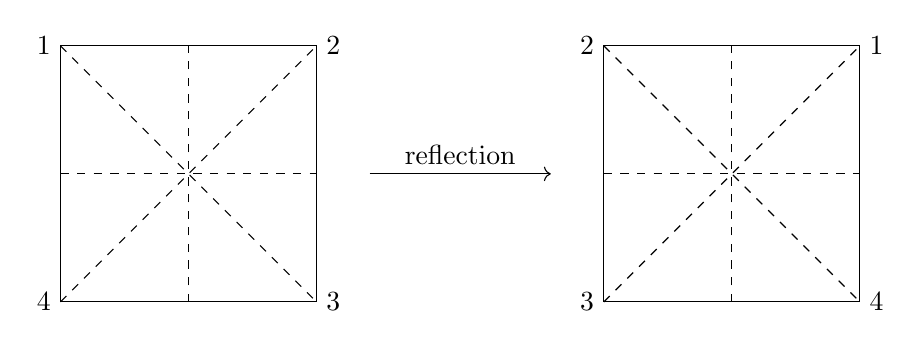
\begin{tikzpicture}[scale=1.15]
		\draw (-3,0)  +(45:2) node [right] {2} -- +(135:2) node [left] {1} -- +(225:2) node [left] {4} -- +(315:2) node [right] {3} -- cycle;
		\draw[dashed] (-3,-1.414) -- (-3,1.414);
		\draw[dashed] (-4.414,0) -- (1.414-3,0);
		\draw[dashed] (-4.414,1.414) -- (1.414-3,-1.414);
		\draw[dashed] (-4.414,-1.414) -- (1.414-3,1.414);
		\draw (3,0)  +(45:2) node [right] {1} -- +(135:2) node [left] {2} -- +(225:2) node [left] {3} -- +(315:2) node [right] {4} -- cycle;
		\draw[dashed] (-3+6,-1.414) -- (-3+6,1.414);
		\draw[dashed] (-4.414+6,0) -- (1.414-3+6,0);
		\draw[dashed] (-4.414+6,1.414) -- (1.414-3+6,-1.414);
		\draw[dashed] (-4.414+6,-1.414) -- (1.414-3+6,1.414);
		\draw[->] (-1,0) -- (1,0);
		\node [above] at (0,0) {{reflection}};
	\end{tikzpicture}
	\caption{The symmetries of a square and a reflection about the vertical line of symmetry.}
\end{figure}
This gives us an intuitive understanding of groups: they encode the symmetries of mathematical objects.

%%%%%%%%%%%%%%%%%%%%%%%%%%%%%%%%%%%%%%%%%%%%%%%%%%%%%%%%%%%%%%%%%%%%%%%%%%%%%%%%%%%%%%%%%%%%%%

\subsection*{What is representation theory?}
The study of groups yields insight into geometric objects.
The action of the dihedral group on the $m$-gon serves as example of a group acting on a geometric object.
More generally, we can consider the action of a group on some object.
Specifically, we say that a group $G$ \emph{acts} on a set $X$ if, for each $g\in G$, there is a map $\cdot\colon G\times X\to X$ satisfying $1_G\cdot x = x$ and $g\cdot (h\cdot x) = (gh)\cdot x$ for all $x\in X$.
Alternatively, one can view this as a group homomorphism $\rho\colon G\to \Sym(X)$, where $\Sym(X)$ is the symmetric group associated to $X$, i.e.\ the group of permutations of elements of $X$.

Now we linearise the setting above by requiring that $X=V$ is a \emph{vector space}.
Then we say that $G$ acts \emph{linearly} on $V$ if there exists a group homomorphism $\rho\colon G\to \GL(V)$.
We call $(V,\rho)$ a \emph{representation} of $G$, and $\rho$ is often suppresed from notation.
We see that $G$ acts on $V$ in the sense that $\rho(g)\colon V\to V$ is a linear invertible map on $V$.
We may denote $\rho(g)(v)$ by $g\cdot v$ as before.

Representation theory is concerned with understanding and classifying linear actions of groups.
The general situation of representation theory is as follows.
If the group $G$ acts on a vector space $V$, then we say that a vector subspace $W\subseteq V$ is a \emph{subrepresentation} of $V$ if it is invariant under the action of $G$.
A representation is called \emph{irreducible} if its only proper subrepresentation is the trivial representation $W=\{0\}$.
The primary goals of representation theory are finding all irreducible representations of $G$, and to decompose a given representation into its irreducible components.

We can think of irreducible representations as the building blocks of all other representations.
This is a common idea in mathematics, seen in other areas.
For instance, in number theory, the building blocks of integers are primes and, in group theory, the building blocks of groups are simple groups.

Writing a general representation in terms of irreducible components is not always possible.
We call a representation \emph{decomposable} if we can write it as the direct sum of irreducible representations.
A lot can be said about the case where the representation of a finite group is over a field whose characteristic not dividing the order of the group.
In this case, \emph{Maschke's theorem} tells us that these representations are always decomposable \cite{Lang02}.
In particular, complex representations of a finite group are always decomposable.

%%%%%%%%%%%%%%%%%%%%%%%%%%%%%%%%%%%%%%%%%%%%%%%%%%%%%%%%%%%%%%%%%%%%%%%%%%%%%%%%%%%%%%%%%%%%%%

\subsection*{Gelfand Pairs}
Henceforth, we assume some knowledge of abstract algebra from the reader.
Let $G$ be a finite group and $K\leq G$ a subgroup.
The pair $(G,K)$ is called a \emph{Gelfand pair} if the induced representation $\Ind_K^G \1$ is multiplicity-free.
Here $\1$ denotes the trivial ($1$-dimensional) complex representation of $K$, and multiplicity-free means that any irreducible representation appears in the decomposition of $\Ind_K^G \1$ at most once (up to isomorphism).

Gelfand pairs play an important role in representation theory \cites{Musili93}, analysis \cites{Koranyi80,Morel18}, combinatorics \cite{Bannai84}, number theory \cites{Gross91, Terras99} and probability \cites{CSST20, Diaconis88}.
One of our objectives is to give a detailed study of Gelfand pairs of finite groups.
A main theorem of this thesis is the following:
\begin{thm}(Gelfand's Trick)\label{theorem: Gelfands_Trick_intro}
	Let $G$ be a finite group and $K$ a subgroup of $G$.
	Suppose $\varphi\colon G\to G$ is an involutive anti-automorphism (i.e.\ a bijective anti-homomorphism) such that $K\varphi(x)K=KxK$ for all $x\in G$.
	Then $(G,K)$ is a Gelfand pair.
\end{thm}
The theorem above is proved using the \emph{Hecke algebra}.
There are multiple constructions of Hecke algebras in the  literature \cites{CMHL03,CSST20}.

%%%%%%%%%%%%%%%%%%%%%%%%%%%%%%%%%%%%%%%%%%%%%%%%%%%%%%%%%%%%%%%%%%%%%%%%%%%%%%%%%%%%%%%%%%%%%%

\subsection*{Types of Hecke algebras}
Another objective of this thesis is to present these a priori different Hecke algebras and resolve their apparent discrepancies.
For instance, one way to define the Hecke algebra is as a convolution algebra of $K$-bi-invariant complex-valued functions $f\colon G\to\CC$ on a group.
Another way to define the Hecke algebra is as the algebra generated by $n-1$ variables $T_1,\ldots T_{n-1}$ subject to a \emph{quadratic relation} $T_i^2 = (q-1)T_i + q$ and a \emph{braid relation}
\[
	\underbrace{T_iT_jT_i\ldots}_{m_{ij}\ \text{terms}}=\underbrace{T_jT_iT_j\ldots}_{m_{ij}\ \text{terms}}.
\]
Here $m_{ij}$ is the $ij^\text{th}$ entry in the \emph{Coxeter matrix} associated to the \emph{Weyl group} of $G$. The name `braid relation' is due to a method of visualising the \emph{symmetric group} $S_n$.
If $n$ is a positive integer then the group $S_n$ is the collection of bijections on the set $\{1,2,\ldots,n\}$ to itself, with the group operation of composing functions.
A natural method of visualising elements and multiplication in this group is via \emph{braid diagrams}.
For instance, if $\sigma = (1\ 2)(3\ 5\ 4)$ and $\pi = (1\ 2\ 4\ 6\ 5\ 3)$ are permutations in $S_6$ (written in cycle notation), then we may visualise these elements and their product $\pi\sigma = (1\ 4)(5\ 6)$ in the following manner:
\begin{figure}[H]
	\[
		\begin{pdiag}[1.5]{6}{2}
			\pdiagfill
			\pdiagmap{1}{2}
			\pdiagmap{2}{1}
			\pdiagmap{3}{5}
			\pdiagmap{4}{3}
			\pdiagmap{5}{4}
			\pdiagmap{6}{6}
			\pdiagname{$\sigma$}
			\pdiagendmap
			\pdiagmap{1}{2}
			\pdiagmap{2}{4}
			\pdiagmap{3}{1}
			\pdiagmap{4}{6}
			\pdiagmap{5}{3}
			\pdiagmap{6}{5}
			\pdiagname{$\pi$}
		\end{pdiag}
		=
		\begin{pdiag}[1.5]{6}{1}
			\pdiagfill
			\pdiagmap{1}{4}
			\pdiagmap{2}{2}
			\pdiagmap{3}{3}
			\pdiagmap{4}{1}
			\pdiagmap{5}{6}
			\pdiagmap{6}{5}
		\end{pdiag}
	\]
	\caption{A braid diagram visualising the multiplication $\pi\sigma = (1\ 4)(5\ 6)$.}
\end{figure}

%%%%%%%%%%%%%%%%%%%%%%%%%%%%%%%%%%%%%%%%%%%%%%%%%%%%%%%%%%%%%%%%%%%%%%%%%%%%%%%%%%%%%%%%%%%%%%

\subsection*{Why study Hecke algebras?}
The Hecke algebra arises naturally when one wishes to compute certain irreducible representations of a group \cite{Williamson21,CMHL03}.
Consider a finite group $G$ and a normal subgroup $N\triangleleft G$.
If $G$ acts linearly on a vector space $V$ (i.e.\ $V$ is a representation of $G$), then there is a natural action of $G$ on the subrepresentation $V^N$, the space of vectors in $V$ that are fixed by $N$.
Under this action, $N$ will clearly act trivially on $V^N$.
This yields a representation of the quotient group $G/N$.
After some representation theoretic arguments, one arrives at the conclusion that
\[
	\left\{\begin{array}{c}
		\text{Irreducible representations} \\
		\text{of $G$ with $N$-fixed vectors}
	\end{array}\right\}
	\stackrel{1:1}{\longleftrightarrow}
	\left\{\begin{array}{c}
		\text{Irreducible representations} \\
		\text{of $G/N$}
	\end{array}\right\}.
\]
It is a straightforward exercise that a complex representation of the group $G/N$ is the same as a representation of the algebra $\CC[G/N]$, the \emph{group algebra} of $G/N$.

What happens when we do not require a normal subgroup of $G$? Consider an arbitrary subgroup $K$ of a finite group $G$.
Now $G/K$ is no longer necessarily a group, so $G/K$ and $\CC[G/K]$ no longer necessarily make sense.
We ask ourselves: what acts on $V^K$?
The action of $G$ on $V$ is not well-defined on $V^K$ since $K$ is no longer normal.
It is not obvious how we could study irreducible $G$-representations with $K$-fixed vectors.
We are able to salvage the situation with the help of the Hecke algebra.

For $g\in G$, define the Hecke operator $[KgK] := \frac{1}{|K|}\sum_{x\in KgK} x\in\CC[G]$, which acts on $V^K$ by
\[
	[KgK]\cdot v := \frac{1}{|K|}\sum_{x\in KgK} x\cdot v.
\]
Now define the Hecke algebra $\calH(G,K)$ to be the space of functions $f\colon G\to\CC$ that are constant on $K$-double cosets.
The indicator functions $\chi_{KgK}$ form a basis of this space and we can uniquely associate the indicator functions $\chi_{KgK}$ to the Hecke operators $[KgK]$.
We see that, through the Hecke operators, we have defined an action of $\calH(G,K)$ on $V^K$.
This answers our question of what acts on $V^K$.
Through another representation-theoretic exercise, one can conclude that
\[
	\left\{\begin{array}{c}
		\text{Irreducible representations} \\
		\text{of $G$ with $K$-fixed vectors}
	\end{array}\right\}
	\stackrel{1:1}{\longleftrightarrow}
	\left\{\begin{array}{c}
		\text{Irreducible representations} \\
		\text{of $\calH(G,K)$}
	\end{array}\right\}.
\]
An immediate example of the utility of this result is as follows. It is easy to show that if $\calH(G,K)$ is commutative, then all of its irreducible finite-dimensional representations are one-dimensional \cite{Etingof11}.
The commutativity of the Hecke algebra turns out to be an important property which will be investigated throughout this thesis.

%%%%%%%%%%%%%%%%%%%%%%%%%%%%%%%%%%%%%%%%%%%%%%%%%%%%%%%%%%%%%%%%%%%%%%%%%%%%%%%%%%%%%%%%%%%%%%

\subsection*{Contents of this thesis}
In Chapter \ref{Chapter1}, we begin our study of the Hecke algebra.
First, we investigate the convolution algebra of all complex-valued functions on $G$ and its ideal of $K$-right-invariant complex-valued functions.
This is followed by results describing the relationship between the induced representation and its associated Hecke algebra.
We use these results to prove Theorem \ref{theorem: Gelfands_Trick_intro}.
This allows us to write down simple proofs that $\Ind_K^G \1$ is multiplicity-free for certain choices of $G$ and $K$.
Namely, $(G,K)$ with $G$ commutative, $(G,K)$ with $[G\! :\! K]=2$, $(S_{n+m}, S_n\times S_m)$, and $(O_{n+1}(\FF_q), O_n(\FF_q))$ for $q$ odd.

In Chapter \ref{Chapter2}, we generalise the discussion of Chapter 1 to the case of a non-trivial \emph{character} $\sigma\colon K\to\CC^\times$.
Here our goal is to obtain a twisted analogue of Theorem \ref{theorem: Gelfands_Trick_intro}.
To this end, we describe the basis of the Hecke algebra using the idea of \emph{relevant orbits}.
We state and prove the generalisation of Theorem \ref{theorem: Gelfands_Trick_intro}.
We apply the new theorem to a particular representation, the \emph{Gelfand--Graev representation} of $\GL_n(\FF_q)$, to show that it is multiplicity-free.

In Chapter \ref{Chapter3}, we investigate the Hecke algebra of Chapter \ref{Chapter1} under the particular choice of $G=\SL_n(\FF_q)$ and $K=B(\FF_q)$, the \emph{Borel subgroup} of $G$, i.e.\ the subgroup of upper-triangular matrices.
The \emph{Weyl group} associated to $G$ is introduced and shown to be isomorphic to $S_n$.
Next, we perform some elementary matrix calculations which yields the surprising result above: the Hecke algebra may be written in terms of $n-1$ generators subject to the quadratic relation and the braid relations associated to $W$.
This leads to a concluding discussion of Hecke algebras generated by any finite \emph{Coxeter group}.

In Chapter \ref{Chapter4}, we generalise the results of earlier chapters to the case where $G$ is no longer finite, but instead a locally compact topological group.
This allows for an extension of the theory we have developed to more general groups and their Hecke algebras.
To do this, we discuss how one can impose a topological structure on a group and supply examples to give some intuition for these types of groups.
To define Hecke algebras of these groups, we require some measure theory.
In particular, the convolution product on the Hecke algebra is defined in terms of an integral with respect to the \emph{Haar measure}.
We spend some time developing the theory of Haar measures for this purpose.
We conclude with a discussion of how to recover the Hecke algebra of a finite group from this new definition.
In this chapter, we shall denote the Hecke algebra by $C_c(K\backslash G/K)$ to emphasise the non-finiteness of $G$.

In Chapter \ref{Chapter5}, we take a look at some specific Hecke algebras of locally compact topological groups.
In particular, we restrict our attention to the general linear group over a non-archimedian local field $k$ and its ring of integers $\calO$.
We look at the \emph{Spherical Hecke algebra}, formed when one considers $G=\GL_n(k)$ and $K=K^\circ := \GL_n(\calO)$, and the \emph{Iwahori--Hecke algebra}, formed when one considers $G=\GL_n(\calO)$ and $K=I$, the \emph{Iwahori subgroup}.
In order to investigate these algebras, we must develop an understanding of these fields.
We detail their definition, classification and structure.

The contents of this thesis may be visualised with the following diagram.
\begin{figure}[H]
	% https://q.uiver.app/?q=WzAsNixbMSwwLCJcXGNhbEgoRyxLKSJdLFsyLDAsIkNfYyhLXFxiYWNrc2xhc2ggRy9LKSJdLFszLDAsIkNfYyhJXFxiYWNrc2xhc2ggRy9JKSJdLFswLDAsIlxcY2FsSChHLEssXFxzaWdtYSkiXSxbMSwxLCJcXGNhbEhfcShXLFMpIl0sWzIsMSwiQ19jKEteXFxjaXJjXFxiYWNrc2xhc2ggRy9LXlxcY2lyYykiXSxbMSw1LCJLPUteXFxjaXJjIl0sWzEsMCwiR1xcIFxcdGV4dHtmaW5pdGV9IiwyXSxbMSwyLCJLPUkiXSxbMCw0LCJHXFwgXFx0ZXh0e0xpZSB0eXBlfSJdLFszLDAsIlxcc2lnbWE9XFwxIl1d
	\[
		\begin{tikzcd}
			{\overset{\text{Ch.\ \ref{Chapter2}}}{\calH(G,K,\sigma)}} & {\overset{\text{Ch.\ \ref{Chapter1}}}{\calH(G,K)}} & {\overset{\text{Ch.\ \ref{Chapter4}}}{C_c(K\backslash G/K)}} & {\overset{\text{Ch.\ \ref{Chapter5}}}{C_c(I\backslash G/I)}} \\
			& {\underset{\text{Ch.\ \ref{Chapter3}}}{\calH_q(W,S)}} & {\underset{\text{Ch.\ \ref{Chapter5}}}{C_c(K^\circ\backslash G/K^\circ)}}
			\arrow["{K=K^\circ}", from=1-3, to=2-3]
			\arrow["{G\ \text{finite}}"', from=1-3, to=1-2]
			\arrow["{K=I}", from=1-3, to=1-4]
			\arrow["{\substack{G\ \text{Lie type}\\ \text{over}\ \FF_q}}", from=1-2, to=2-2]
			\arrow["{\sigma=\1}", from=1-1, to=1-2]
		\end{tikzcd}
	\]
	\caption{The relationship diagram of this thesis.}
\end{figure}

%%%%%%%%%%%%%%%%%%%%%%%%%%%%%%%%%%%%%%%%%%%%%%%%%%%%%%%%%%%%%%%%%%%%%%%%%%%%%%%%%%%%%%%%%%%%%%

\subsection*{Directions for future research}
We assume the reader is familiar with the contents of this thesis.
The modern study of Hecke algebras is largely focused on the \emph{Iwahori--Hecke algebra}, which is also known as the \emph{affine Hecke algebra}.
This algebra is central to the study of representations of \emph{reductive groups} over non-archimedian local fields (e.g.\ groups such as $\GL_n$, $\SL_n$, $\Sp_{2n}$ over fields such as $\QQ_p$ or $\FF_q(\!(t)\!)$).

Some topics relevant to the Iwahori--Hecke algebra include \emph{Bernstein's presentation}, the \emph{Iwahori--Matsumoto presentation} and the \emph{Satake isomorphism} \cite{HKP}.
Properties of the Iwahori--Hecke algebra such as these presentations may be viewed as a consequence of the \emph{universal unramified principal series module}, which we now describe.

Fix a ``nice'' (i.e.\ split and connected) reductive group $G$ (e.g.\ $\SL_n$) over a non-archimedian local field $k$ with ring of integers $\calO$.
Then write $A$ to mean a \emph{split maximal torus} of $G$ and write $N$ to mean the \emph{unipotent radical} of a Borel subgroup of $G$ that contains $A$.
Also recall $I$ is the Iwahori subgroup of $G$ given in Chapter \ref{Chapter5}.

The universal unramified principal series module $M$ is given by $C_c(A(\calO)N\backslash G/I)$.
It is a right module over the Iwahori--Hecke algebra under convolution.
Furthermore, a basis of the Iwahori--Hecke algebra is parameterised by the \emph{affine Weyl group} $\widetilde{W}$.
We may write $\widetilde{W} \cong W \ltimes \Lambda^\vee$, where $\Lambda^\vee$ is the \emph{coroot lattice} of $G$.
Then $\CC[\Lambda^\vee]$ is the corresponding group algebra over $\CC$.
Then $M$ is also a left module over $\CC[\Lambda^\vee]$.

\newpage
\addtocontents{toc}{\protect\setcounter{tocdepth}{2}}

% blank page
\
\newpage
%%%%%%%%%%%%%%%%%%%%%%%%%%%%%%%%%%%%%%%%%%%%%%%%%%%%%%%%%%%%%%%%%%%%%%%%%%%%%%%%%%%%%%%%%%%%%%

\section{Hecke Algebras of Finite Groups}\label{Chapter1}
The aim of this chapter is to study the structure of the Hecke algebra and elucidate its significance in the representation theory of $G$.

In Section \ref{Section1.1}, we introduce $(\Fun(G),\star)$, the convolution algebra of functions from $G$ to $\CC$.
In Section \ref{Section1.2}, we present and discuss the induced representation $\Ind_K^G\1$ and its underlying vector space, $W$.
In Section \ref{Section1.3}, we introduce the Hecke algebra, $\calH(G,K)$.
This is the space of functions that are constant on $K$-double cosets.
In Section \ref{Section1.4}, we present the group algebra $\CC[G]$, which is isomorphic to $\Fun(G)$, and describe the copies of $W$ and $\calH(G,K)$ that lie inside of $\CC[G]$.
In Section \ref{Section1.5}, we make the fundamental observation that $\calH(G,K)\cong\End_G(W)$, the endomorphism algebra of $G$-intertwiners on $W$.
This is crucial for the final section, Section \ref{Section1.6}, where we prove that a representation $V$ is multiplicity-free if and only if $\End_G(V)$ is commutative.
This lets us conclude that the induced representation $W$ is multiplicity-free if and only if its associated Hecke algebra is commutative.

The purpose of Section \ref{Section1.7} is to develop a tool to expedite the process of proving $\calH(G,K)$ is commutative.
This tool comes in the form of Gelfand's Trick, which transforms the task of proving commutativity into the task of writing down an involutive anti-automorphism of $G$ that preserves $K$-double cosets.
We will see that this is a much easier task to perform.
To prove Gelfand's Trick, we investigate the behavior of anti-automorphisms on $G$ and $\Fun(G)$.
As we do this, the required conditions for Gelfand's Trick reveal themselves, leading to a natural statement and proof.
We conclude with some examples of applications of the main theorem in Section \ref{Section1.8}.

%%%%%%%%%%%%%%%%%%%%%%%%%%%%%%%%%%%%%%%%%%%%%%%%%%%%%%%%%%%%%%%%%%%%%%%%%%%%%%%%%%%%%%%%%%%%%%

\subsection{The convolution algebra of functions $\Fun(G)$}\label{Section1.1}
Let $X$ be a finite set.
Denote the vector space of complex-valued maps on $X$ by $\Fun(X) := \{f\colon X\to \CC\}$.
It has a basis of delta functions $\{\delta_x\}_{x\in X}$ defined by $\delta_x(x)=1$ and $\delta_x(y)=0$ for $y\neq x$.
Note that $\Fun(X)$ is a commutative unital associative algebra under pointwise multiplication of functions.
Also note that if a group $G$ acts on $X$, then $G$ also acts on $\Fun(X)$ by $(g\cdot f)(x) := f(g^{-1}\cdot x)$.
Thus, $\Fun(X)$ is a representation of $G$.

Now suppose that $X=G$ is a finite group.
The group structure on $G$ yields a second algebra structure on $\Fun(G)$.
Specifically, it has the convolution product defined by
\[
	(f\star f')(x) := \sum_{yz = x} f(y)f'(z) = \sum_{g\in G} f(xg)f'(g^{-1}).
\]
One can show that $\star$ is associative with identity $\delta_{1_G}$, so $(\Fun(G),\star)$ is a unital associative algebra.
It is easy to see that this algebra is commutative if and only if $G$ is commutative.

%%%%%%%%%%%%%%%%%%%%%%%%%%%%%%%%%%%%%%%%%%%%%%%%%%%%%%%%%%%%%%%%%%%%%%%%%%%%%%%%%%%%%%%%%%%%%%

\subsection{The induced representation $\Ind_K^G \1$}\label{Section1.2}
Consider the space of functions in $\Fun(G)$ that are invariant under right-multiplication by elements of $K$.
Explicitly, this space is defined by
\[
	W: = \{f\colon G\to \CC\ |\ f(gk) = f(g),\ \forall g\in G, \forall k \in K\} \subseteq \Fun(G).
\]
Note that the action of $G$ on $\Fun(G)$ leaves $W$ invariant.
The resulting action of $G$ on $W$ is called the \emph{induced representation} and denoted $\Ind_K^G \1$.
When $K=\{1\}$, the representation $\Ind_{\{1\}}^G\1=\Fun(G)$ is the \emph{left regular} representation of $G$.
For future use, we prove the following lemma.
\begin{lem}\label{lemma: W_left_ideal}
	The space $W$ is a left ideal of $(\Fun(G),\star)$.
\end{lem}
\begin{proof}
	We verify that $f\star w\in W$ whenever $w\in W$ and $f\in\Fun(G)$.
	Let $g\in G$ and $k\in K$.
	Then
	\begin{multline*}
		(f\star w)(gk) = \sum_{xy=gk} f(x)w(y) = \sum_{x\in G} f(x)w(x^{-1}gk) \\
		= \sum_{x\in G} f(x)w(x^{-1}g) = \sum_{xy=g} f(x)w(y) = (f\star w)(g).\qedhere
	\end{multline*}
\end{proof}

%%%%%%%%%%%%%%%%%%%%%%%%%%%%%%%%%%%%%%%%%%%%%%%%%%%%%%%%%%%%%%%%%%%%%%%%%%%%%%%%%%%%%%%%%%%%%%

\subsection{The Hecke algebra of a finite group $\calH(G,K)$}\label{Section1.3}
Consider the space of functions in $\Fun(G)$ that are invariant under right- and left-multiplication by elements of $K$.
Explicitly, this space is defined by
\[
	\calH(G,K) := \{f\colon G\to \CC\ |\ f(k_1gk_2) = f(g),\ \forall g\in G,\ \forall k_1,k_2\in K\} \subseteq \Fun(G).
\]
This is the \emph{Hecke algebra} associated to $G$ and $K$ and we will write $\calH$ to mean $\calH(G,K)$ when there is no ambiguity.
The proof of Lemma \ref{lemma: W_left_ideal} can be adapted to show that $\calH$ is a two-sided ideal in $(\Fun(G),\star)$.
Notice that the identity of $(\Fun(G),\star)$ does not lie in $\calH$.
Nevertheless, $\calH$ does have an identity of its own.
It is easy to verify that the identity is $\iota_K$, which we define below.
\[
	\iota_K:G\to\CC,\quad \iota_K(g) := \begin{cases}
		\frac{1}{|K|},\  & \text{if}\ g\in K, \\
		0,\              & \text{else}.
	\end{cases}
\]
We see that $\iota_K$ is an idempotent element, since $(\iota_K\star\iota_K)(g)=0$ for $g\notin K$, and
\[
	(\iota_K\star\iota_K)(k) = \sum_{x\in G} \iota_K(kx)\iota_K(x^{-1}) = \sum_{x\in K} \frac{1}{|K|^2} = \frac{1}{|K|}
\]
for $k\in K$.

This is a special case of a more general situation: if $R$ is a ring and $e$ is an idempotent, then $eRe$ will be a ring in which $e$ serves as a unit.
This is clear since $eree=ere=eere$ for all $ere\in eRe$.
The ring $eRe$ is sometimes called an \emph{idempotented ring} or a \emph{Pierce corner} \cite{Bump10,Lam06}.

We present a basis for $\calH$.
For $KxK\in K\backslash G/K$, the $K$-double cosets in $G$, we define
\[
	\chi_{KxK}(y) := \begin{cases}
		1,\  & \text{if}\ y\in KxK, \\
		0,\  & \text{else}.
	\end{cases}
\]
Recall that double cosets partition $G$ so there is no ambiguity in this definition.
We call $\chi_{KxK}$ the \emph{characteristic function} of the $K$-double coset $KxK$.
As an abuse of notation for the sake of brevity, we will denote this family by $\{\chi_x\}_{x\in G}$, where $x$ ranges over the $K$-double coset representatives as written above.

It is not hard to see that the characteristic functions form a basis of $\calH$.
By the definition of $\calH$, we see characteristic functions span the space.
To see that they're linearly independent, assume that
\[
	\alpha_1 \chi_{x_1} + \cdots + \alpha_n \chi_{x_n}  = 0,
\]
for some complete collection of $K$-double coset representatives $x_i\in G$ and scalars $\alpha_i\in\CC$.
Here $0$ denotes the zero function $g\mapsto 0$ for all $g\in G$.
Evaluating both sides at $x_i$ tells us that $\alpha_i=0$, so the only solution is the trivial solution and we have linear independence.

%%%%%%%%%%%%%%%%%%%%%%%%%%%%%%%%%%%%%%%%%%%%%%%%%%%%%%%%%%%%%%%%%%%%%%%%%%%%%%%%%%%%%%%%%%%%%%

\subsection{The group algebra $\CC[G]$}\label{Section1.4}
We can associate to $G$ another algebra, $\CC[G]$, called the \emph{group algebra} of $G$ over $\CC$.
This algebra is defined by
\[
	\CC[G] := \Bigg\{ \sum_{g\in G} a_g e_g\ \Bigg|\ a_g\in \CC \Bigg\}.
\]
Clearly, the set $\{e_g\}_{g\in G}$ serves as a basis of this space.
We endow the space with a multiplication defined on basis elements by $e_ge_h := e_{gh}$.
The following lemma illustrates the relevance of the group algebra.
\begin{lem}
	The map $\Phi\colon \Fun(G)\to\CC[G]$ defined on basis elements by $\delta_g\mapsto e_g$ and extended linearly is an algebra isomorphism.
\end{lem}
\begin{proof}
	By construction, $\Phi$ is a linear map of vector spaces.
	It is also clear that this map is bijective since it is a bijection on basis elements.
	Thus $\Phi$ is a vector space isomorphism.

	We need to check that $\Phi$ respects the algebra multiplication.
	This amounts to verifying that $\delta_g \star \delta_h = \delta_{gh}$.
	Notice that $(\delta_g\star\delta_h)(x) = \sum_{ab=x} \delta_g(a)\delta_h(b)$ is equal to $1$ when $g=a$ and $h=b$, and $0$ otherwise.
	This is exactly $\delta_{gh}(x)$.
\end{proof}
We may ask ourselves: what is the image of the induced representation and the Hecke algebra inside of the group algebra? To answer this, we define the group algebra element
\[
	e := \frac{1}{|K|} \sum_{k\in K} e_k.
\]
Note that $e$ is an idempotent element.
Then the following proposition answers our question.
\begin{prop}
	\begin{enumerate}[\itshape(i)]
		\item $\Phi(W) = \CC[G]e$.
		\item $\Phi(\calH) = e \CC[G] e$.
	\end{enumerate}
\end{prop}
\begin{proof}
	\begin{enumerate}[\itshape(i)]
		\item We begin by showing that $\CC[G]e\subseteq \Phi(W)$.
		      To see this, take an arbitrary element $(\sum_{g\in G} a_ge_g)e$ in $\CC[G]e$.
		      Then notice
		      \[
			      \bigg(\sum_{g\in G} a_ge_g\bigg)e = \frac{1}{|K|}\bigg(\sum_{g\in G} a_ge_g\bigg)\bigg(\sum_{k\in K}e_k\bigg) = \frac{1}{|K|}\sum_{\substack{g\in G \\ k\in K}} a_ge_ge_k = \frac{1}{|K|}\sum_{\substack{g\in G \\ k\in K}} a_ge_{gk}.
		      \]
		      Then we apply $\Phi^{-1}$ to see that
		      \[
			      \frac{1}{|K|}\sum_{\substack{g\in G \\ k\in K}} a_ge_{gk} \mapsto \frac{1}{|K|}\sum_{\substack{g\in G \\ k\in K}} a_g\delta_{gk}.
		      \]
		      We wish to show that this lies in $W$, so we wish to check that this map is invariant under right-multiplication by an element of $K$.
		      To this end, let $g'\in G$, $k'\in K$ and apply $\frac{1}{|K|}\sum_{\substack{g\in G \\ k\in K}} a_g\delta_{gk}$ to $g'k'$.
		      Note that $\delta_{gk}(g'k')=1$ if and only if $gk=g'k'$ (and $0$ otherwise).
		      This is equivalent to $g=g'k'k^{-1}$.
		      Thus
		      \[
			      \frac{1}{|K|}\sum_{\substack{g\in G \\ k\in K}} a_g\delta_{gk}(g'k') = \frac{1}{|K|}\sum_{k\in K} a_{g'k'k^{-1}}\delta_{g'k'}(g'k') = \frac{1}{|K|}\sum_{k\in K} a_{g'k'k^{-1}}.
		      \]
		      Similarly, we apply the map $\frac{1}{|K|}\sum_{\substack{g\in G \\ k\in K}} a_g\delta_{gk}$ to $g'$.
		      This yields
		      \[
			      \frac{1}{|K|}\sum_{\substack{g\in G \\ k\in K}} a_g\delta_{gk}(g') = \frac{1}{|K|}\sum_{k\in K} a_{g'k^{-1}}
		      \]
		      Since right-multiplication by any element of $K$ is an automorphism of $G$, we see that
		      \[
			      \frac{1}{|K|}\sum_{k\in K} a_{g'k'k^{-1}}=\frac{1}{|K|}\sum_{k\in K} a_{g'k^{-1}},
		      \]
		      which shows that $\CC[G]e\subseteq \Phi(W)$.
		      Conversely, take $f=\sum_{g\in G} a_g\delta_g\in W$.
		      Let $g'\in G$, $k'\in K$ and notice that
		      \[
			      a_{g'k'} = \sum_{g\in G} a_g\delta_g(g'k') = f(g'k') = f(g') = \sum_{g\in G} a_g \delta_g(g') = a_{g'}.
		      \]
		      Then $a_{g'k'}=a_{g'}$ for any $g'\in G$ and $k'\in K$.
		      Then observe
		      \begin{multline*}
			      \Phi(f)e = \bigg(\sum_{g\in G} a_g\delta_g\bigg)\bigg(\frac{1}{|K|}\sum_{k\in K} e_k\bigg) = \frac{1}{|K|} \sum_{\substack{g\in G \\ k\in K}} a_g e_{gk} = \frac{1}{|K|} \sum_{\substack{g\in G \\ k\in K}} a_{gk^{-1}} e_g \\
			      = \frac{1}{|K|} \sum_{\substack{g\in G \\ k\in K}} a_g e_g = \frac{1}{|K|}\sum_{k\in K}\sum_{g\in G} a_ge_g = \frac{1}{|K|}\sum_{k\in K} \Phi(f) = \Phi(f).
		      \end{multline*}
		      Then $\varphi(f)=\varphi(f)e\in\CC[G]e$, so $\Phi(W)\subseteq \CC[G]e$ as required.

		\item The proof is similar to that of {\itshape(i)}.\qedhere
	\end{enumerate}
\end{proof}

%%%%%%%%%%%%%%%%%%%%%%%%%%%%%%%%%%%%%%%%%%%%%%%%%%%%%%%%%%%%%%%%%%%%%%%%%%%%%%%%%%%%%%%%%%%%%%

\subsection{Identifying $\calH(G,K)$ with the endomorphism algebra $\End_G(W)$}\label{Section1.5}
For any representation $V$ of $G$, define the space of \emph{$G$-intertwining endomorphisms on $V$} by
\[
	\End_G(V) := \{ f\in\End(V)\ |\ g\cdot f(v) = f(g\cdot v),\ \forall\ v\in V,\ g\in G \}\subseteq \End(V).
\]
These are the endomorphisms of $V$ that respect the action of $G$ on $V$.
It is easy to see that this is a vector space.
It has the additional structure of a unital associative algebra when endowed with the product of endomorphism composition.

Now set $V$ to be $W$, the induced representation of the trivial character from $K$ to $G$, and define the linear map
\[
	\Psi\colon \calH\to\End(W),\quad \alpha\mapsto(w\mapsto w\star\alpha).
\]
Lemma \ref{lemma: W_left_ideal} tells us that $w \star\alpha$ is indeed an element of $W$ so the image of $\Psi$ is indeed $\End(W)$.
The following proposition highlights the significance of this map.
\begin{prop}\label{prop: H_iso_End_G(W)}
	The map $\Psi$ defines an algebra isomorphism $\calH \cong \End_G(W)$.
\end{prop}
\begin{proof}
	First we observe that $\Psi(\alpha)$ is indeed a $G$-intertwiner.
	Given $g,h\in G$ and $w\in W$, we have
	\begin{multline*}
		(\Psi(\alpha)(g\cdot w))(h) = ((g\cdot w)\star\alpha)(h) = \sum_{xy=h} w(g^{-1}x)\alpha(y) = \sum_{x\in G} w(g^{-1}x)\alpha(x^{-1}h) \\
		= \sum_{ab=g^{-1}h} w(a)\alpha(b) = (g\cdot(w\star\alpha))(h) = (g\cdot \Psi(\alpha)(w))(h).
	\end{multline*}
	Thus, the image of $\Psi$ lies in $\End_G(W)$.
	Next, we check that $\Psi$ is an algebra isomorphism.
	Let $\alpha_1,\alpha_2\in\calH$ and observe
	\[
		\Psi(\alpha_1\star\alpha_2)(w) = w\star(\alpha_1\star\alpha_2) = (w\star\alpha_1)\star\alpha_2 = \Psi(\alpha_1)(w)\star\alpha_2 = (\Psi(\alpha_1)\circ\Psi(\alpha_2))(w).
	\]
	Thus $\Psi$ is an algebra homomorphism.
	To see that $\Psi$ is injective, we compute
	\[
		\ker \Psi = \{\alpha\in\calH\ |\ \Psi(\alpha)(w) = w\} = \{\alpha\in\calH\ |\ w\star\alpha = w\} = \{\delta_{1_G}\}.
	\]
	We see that $\Psi$ has trivial kernel so it is injective.
	It is easy to see that surjectivity is a consequence of Theorem 13 in \cite{Murnaghan05} which also contains its proof.
\end{proof}

%%%%%%%%%%%%%%%%%%%%%%%%%%%%%%%%%%%%%%%%%%%%%%%%%%%%%%%%%%%%%%%%%%%%%%%%%%%%%%%%%%%%%%%%%%%%%%

\subsection{Consequences for representation theory}\label{Section1.6}
We prove a general property of representations.
Namely, the decomposition of a representation is linked to its corresponding algebra of $G$-intertwining endomorphisms.
We apply this to the induced representation $W$ and Proposition \ref{prop: H_iso_End_G(W)} lets us conclude that $W$ is multiplicity-free if and only if $\calH$ is commutative.

First, suppose that $V$ is a complex representation of $G$.
Write $V = \bigoplus_{i=1}^n V_i$ as the decomposition of $V$ into irreducible constituents, using Maschke's theorem.
Notice that some of these $V_i$ may be isomorphic to each other as $G$-representations.
We group these mutually isomorphic irreducible representations together by writing
\[
	V = \bigoplus_{i=1}^n V_i = \bigoplus_{i=1}^n U_i^{\oplus m_i},
\]
where $m_i$ is the number of times $U_i$ appears in the decomposition of $V$, henceforth referred to as the \emph{multiplicity} of $U_i$ in $V$.
We say $V$ is \emph{multiplicity-free} if $m_i=1$ for all $i$.
The $U_i^{\oplus m_i}$ are called the \emph{isotypical components} of $V$.
We now prove the main proposition of this section.
\begin{prop}\label{prop: V_mult-free_iff_End_G(V)_commutative}
	\begin{enumerate}[\itshape(i)]
		\item If $V$ is a representation of $G$ with the decomposition into isotypical components as above, then $\End_G(V)\cong \bigoplus_{i=1}^n \Mat_{m_i}(\CC)$.
		\item $V$ is multiplicity-free if and only if $\End_G(V)$ is commutative.
	\end{enumerate}
\end{prop}
\begin{proof}
	\begin{enumerate}[\itshape(i)]
		\item Observe that
		      \[
			      \End_G(V) = \Hom_G(V_1\oplus \cdots \oplus V_n, V_1\oplus \cdots \oplus V_n) \cong \bigoplus_{i,j=1,\ldots,n} \Hom_G(V_i, V_j).
		      \]
		      Then we compute
		      \[
			      \Hom_G(V_i,V_j) = \Hom_G(U_i^{\oplus m_i}, U_j^{\oplus m_j}) \cong \Hom_G(U_i,U_j)^{\oplus m_im_j}.
		      \]
		      Schur's lemma tells us that
		      \[
			      \Hom_G(U_i,U_j) \cong \begin{cases}
				      \CC,\    & \text{if}\ U_i\cong U_j,     \\
				      \{0\},\  & \text{if}\ U_i\not\cong U_j.
			      \end{cases}
		      \]
		      Then $\Hom_G(U_i,U_j)^{\oplus m_im_j} =\{0\}$ if $i\neq j$ and
		      \[
			      \Hom_G(U_i,U_i)^{\oplus m_i^2} \cong \CC^{m_i^2} \cong \Mat_{m_i}(\CC).
		      \]
		      Thus $\End_G(V) \cong \bigoplus_{i=1}^n \Mat_{n_i}(\CC)$.

		\item We know from $(i)$ that we can identify $\End_G(V)$ with an algebra of block-diagonal matrices over $\CC$.
		      The sizes of the blocks correspond to $m_i$, the multiplicity of $U_i$ in $V$.
		      Composing two $f,g\in\End_G(V)$ corresponds to multiplying their associated matrices.
		      Then $\End_G(V)$ is commutative if and only if the block sizes are all $1$.
		      That is, if $m_i = 1$ for all $i$. \qedhere
	\end{enumerate}
\end{proof}
\begin{cor}\label{cor: H_commutative}
	\begin{enumerate}[\itshape(i)]
		\item The induced representation $W$ is multiplicity-free if and only if its associated Hecke algebra $\calH$ is commutative.
		\item $W$ is irreducible if and only if $\calH \cong \CC$.
	\end{enumerate}
\end{cor}
\begin{proof}
	\begin{enumerate}[\itshape(i)]
		\item Apply Proposition \ref{prop: V_mult-free_iff_End_G(V)_commutative} with $V=W$.
		      Then $W$ is multiplicity-free if and only if $\End_G(W)$ is commutative.
		      Proposition \ref{prop: H_iso_End_G(W)} tells us that $\End_G(W)\cong\calH$.
		      Thus $W$ is multiplicity-free if and only if $\calH$ is commutative.

		\item Suppose that $W$ is irreducible.
		      Schur's Lemma tells us that $\End_G(W)\cong\CC$, so $\calH\cong\CC$.
		      Conversely, suppose that $\calH\cong\CC$.
		      Write the decomposition of $W$ into irreducible constituents
		      \[
			      W = \bigoplus_{i=1}^n W_i.
		      \]
		      Schur's lemma tells us that $\End_G(W_i)\cong \CC$ for each $i$.
		      Then
		      \[
			      \End_G(W) = \End_G\bigg(\bigoplus_{i=1}^n W_i\bigg) \cong \bigoplus_{i=1}^n \End_G(W_i) \cong \bigoplus_{i=1}^n \CC = \CC^n.
		      \]
		      However $\CC\cong\calH\cong\End_G(W)\cong\CC^n$.
		      Thus $n=1$ and $W$ is irreducible. \qedhere
	\end{enumerate}
\end{proof}

%%%%%%%%%%%%%%%%%%%%%%%%%%%%%%%%%%%%%%%%%%%%%%%%%%%%%%%%%%%%%%%%%%%%%%%%%%%%%%%%%%%%%%%%%%%%%%

\subsection{Gelfand's Trick}\label{Section1.7}
Our goal in this section is to prove the following theorem.
\begin{thm}[Gelfand's Trick] \label{theorem: Gelfand's_Trick}
	Suppose that $G$ is a finite group and $K\leq G$ is a subgroup.
	Let $\varphi\colon G\to G$ be an anti-automorphism with
	\begin{enumerate}[(i)]
		\item $\varphi^2=1$, and
		\item $K\varphi(x)K=KxK$ for all $x\in G$.
	\end{enumerate}
	Then $\calH(G,K)$ is commutative.
\end{thm}
The key idea of this theorem is the following lemma.
\begin{lem}\label{lemma: subalgebra_commutative}
	Let $A$ be an algebra and $B\subseteq A$ be a subalgebra with basis $\{b_i\}_{i\in I}$.
	Suppose $F\colon A\to A$ is an anti-homomorphism (i.e.\ $F(a_1a_2)=F(a_2)F(a_1)$) and $F(b_i) = b_i$.
	Then $B$ is commutative.
\end{lem}
\begin{proof}
	Since $F$ is the identity on basis elements of $B$, there holds $F|_B = \Id_B$.
	Let $b_i,b_j\in B$ be basis elements and notice
	\[
		b_ib_j = F(b_ib_j) = F(b_j)F(b_i) = b_jb_i.
	\]
	Then basis elements of $B$ commute as desired.
\end{proof}
We employ Lemma \ref{lemma: subalgebra_commutative} by applying it to the case where $A=\Fun(G)$ and $B=\calH(G,K)$. Recall from Section \ref{Section1.3} that the characteristic functions $\{\chi_x\}_{x\in G}$ form a basis of $\calH(G,K)$.
\begin{cor}\label{cor: comm}
	Suppose $F\colon \Fun(G) \to \Fun(G)$ is an anti-homomorphism such that $F(\chi_x) = \chi_x$ for all $x\in X$.
	Then $\calH(G,K)$ is commutative.
\end{cor}
This gives us a clear direction going forward: we want to find such a map $F$.

Given an anti-homomorphism of groups $\varphi\colon G\to G$, we can consider the map $\varphi^\ast\colon\Fun(G)\to\Fun(G)$ defined by $\varphi^\ast f := f\circ \varphi$.
This is the \emph{pullback} of $f$ by $\varphi$.
In general, $\varphi^\ast$ is not an anti-homomorphism of convolution algebras.
For instance, consider $G=\ZZ/2\ZZ=\{0,1\}$ and the map $\varphi(x)=x+x=0$.
Clearly $\varphi$ is an anti-homomorphism.
However, consider the maps $f,g\in\Fun(G)$ given by $f(x)=g(x)=0$ if $x=0$ and $f(x)=g(x)=1$ if $x=1$.
Then
\[
	(\varphi^\ast(f\star g))(0) = \sum_{x+y = \varphi(0)} f(x)g(y) = \sum_{x+y = 0} f(x)g(y) = f(0)g(0) + f(1)g(1) = 1,
\]
\[
	((\varphi^\ast g)\star(\varphi^\ast f))(0) = \sum_{x+y = 0} g(\varphi(x))f(\varphi(y)) = \sum_{x+y = 0} g(0)f(0) = 2g(0)f(0) = 0.
\]
Thus $\varphi^\ast$ is not an anti-homomorphism.
However, when $\varphi$ has the stronger anti-automorphism property, we can say the same for $\varphi^\ast$.
More precisely, we have the following lemma.
\begin{lem}
	Suppose $\varphi\colon G\to G$ is a group anti-automorphism.
	Then $\varphi^\ast\colon\Fun(G)\to\Fun(G)$ is an algebra anti-automorphism.
\end{lem}
\begin{proof}
	Let $\varphi$ be a group anti-automorphism.
	Thus $\varphi$ is a bijection and an anti-homomorphism.
	This lets us write $yz=x \iff \varphi(yz)=\varphi(x)$ since $\varphi$ is a bijection.
	We can also write $\varphi(yz)=\varphi(x) \iff \varphi(z)\varphi(y)=\varphi(x)$ since $\varphi$ is an anti-homomorphism.
	Then we compute
	\begin{multline*}
		((\varphi^\ast f)\star(\varphi^\ast g))(x) = \sum_{yz=x} (\varphi^\ast f)(y)(\varphi^\ast g)(z) = \sum_{yz=x} f(\varphi(y)) g(\varphi(z)) = \\
		\sum_{\varphi(z)\varphi(y)=\varphi(x)} g(\varphi(z))f(\varphi(y)) = \sum_{z'y'=\varphi(x)} g(z')f(y') = (\varphi^\ast(g\star f))(x).
	\end{multline*}
	Thus $\varphi^\ast(g\star f) = (\varphi^\ast f)\star(\varphi^\ast g)$.
	We also need to check that $\varphi^\ast$ is a bijection.
	We check this on the basis elements $\{\delta_g\}_{g\in G}$ of $\Fun(G)$.
	Let $g,h\in G$ and we compute
	\[
		(\varphi^\ast\delta_g)(h) = \begin{cases}
			1,\  & \text{if}\ g=\varphi(h), \\
			0,\  & \text{else}.
		\end{cases} = \begin{cases}
			1,\  & \text{if}\ h=\varphi^{-1}(g), \\
			0,\  & \text{else}.
		\end{cases} = \delta_{\varphi^{-1}(g)}(h).
	\]
	We see that $\varphi^\ast$ sends $\delta_g$ to $\delta_{\varphi^{-1}(g)}$.
	We know $\varphi$ and $\varphi^{-1}$ are bijections on $G$, so $\varphi^\ast$ acts bijectively on the basis of $\Fun(G)$.
\end{proof}
Now we know that an anti-automorphism $\varphi$ of $G$ induces an anti-automorphism $\varphi^\ast$ of $\Fun(G)$.
We ask ourselves: when does this anti-automorphism restrict to an anti-automorphism of $\calH(G,K)$?
That is, when is $\varphi^\ast$ also an anti-automorphism of $\calH(G,K)$? The following lemma provides an answer.
\begin{lem}
	Suppose that $\varphi\colon G\to G$ is an anti-automorphism.
	If $\varphi(K)=K$ then $\varphi^\ast$ restricts to an anti-automorphism of $\calH(G,K)$.
\end{lem}
\begin{proof}
	Suppose $f\in\calH$.
	Then notice
	\[
		(\varphi^\ast f)(k_1gk_2) = f(\varphi(k_1gk_2)) = f(\varphi(k_2)\varphi(g)\varphi(k_1)) = f(k_2'\varphi(g)k_1') = f(\varphi(g)) = (\varphi^\ast f)(g).
	\]
	Thus $\varphi^\ast f \in\calH$ since it's constant on $K$-double cosets.
\end{proof}
Now we explore the effect of $\varphi^\ast$ on the basis elements $\{\chi_x\}_{x\in G}$ of $\calH(G,K)$.
\begin{lem}\label{lem: id_on_basis}
	Suppose $\varphi\colon G\to G$ is an anti-automorphism.
	If $\varphi^2=1$ and $K\varphi(x)K=KxK$ for all $x\in G$, then $\varphi^\ast\chi_x=\chi_x$.
\end{lem}
Before we present the proof, notice that $\varphi(K)=K$ is a consequence of the assumption that $K\varphi(x)K=KxK$ for all $x\in G$.
This assumption implies that $K\varphi(x)K=KxK$ for all $x\in K$, which in turn implies that $\varphi(K)=K$.
\begin{proof}
	First, if $g\in KxK$, then
	\[
		\varphi(g)\in \varphi(KxK) = \varphi(K)\varphi(x)\varphi(K) = K\varphi(x)K = KxK.
	\]
	On the other hand, if $\varphi(g)\in KxK$, then
	\[
		g = \varphi(\varphi(g)) \in \varphi(KxK) = \varphi(K)\varphi(x)\varphi(K) = K\varphi(x)K = KxK.
	\]
	We see that $g\in KxK$ if and only if $\varphi(g)\in KxK$.
	Then we compute
	\[
		(\varphi^\ast\chi_x)(g) = \chi_x(\varphi(g)) = \begin{cases}
			1,\  & \text{if}\ \varphi(g)\in KxK, \\
			0,\  & \text{else}.
		\end{cases} = \begin{cases}
			1,\  & \text{if}\ g\in KxK, \\
			0,\  & \text{else}.
		\end{cases} = \chi_x(g).\qedhere
	\]
\end{proof}
We are now ready to prove Theorem \ref{theorem: Gelfand's_Trick}.
\begin{proof}[Proof of Theorem \ref{theorem: Gelfand's_Trick}]
	Lemma \ref{lem: id_on_basis} tells us that $\varphi^\ast$ is the identity on the characteristic functions $\chi_x$.
	These are the basis elements of $\calH(G,K)$.
	Since $\varphi$ is an anti-automorphism, $\varphi^\ast$ will be too.
	We apply Corollary \ref{cor: comm} with $F=\varphi^\ast$ to see that the basis elements commute.
	Thus $\calH(G,K)$ is commutative.
\end{proof}
When applying Gelfand's Trick, we will often consider $\varphi(x)=x^{-1}$ or $\varphi(x)=x^t$ (the latter of which is understood as the transpose map when $G$ is a matrix group).
It is easy to see that they are both involutive anti-automorphisms, so the condition $K\varphi(x)K=KxK$ for all $x\in G$ will be the only condition left to verify.

%%%%%%%%%%%%%%%%%%%%%%%%%%%%%%%%%%%%%%%%%%%%%%%%%%%%%%%%%%%%%%%%%%%%%%%%%%%%%%%%%%%%%%%%%%%%%%

\subsection{Gelfand pairs}\label{Section1.8}
We say that a pair of groups $(G,K)$ with $K\leq G$ is a \emph{Gelfand pair} if $\Ind_K^G \1$ is multiplicity-free.
To be a Gelfand pair, it is sufficient to find an anti-automorphism satisfying the conditions of Theorem \ref{theorem: Gelfand's_Trick}.
We present some examples of applications of this technique.

\subsubsection{Example: $(G,K)$ with $G$ abelian}
For any abelian group $G$, the identity map $\varphi(g)=g$ is an anti-automorphism.
This map clearly satisfies $\varphi^2=1$ and $K\varphi(x)K=KxK$ for all $x\in G$.

\subsubsection{Example: $(G,K)$ with $[G\! :\! K]=2$}
The condition $[G\! :\! K]=2$ tells us that $K$ is a normal subgroup of $G$.
Thus, the quotient group $G/K$ is defined and contains two cosets, $K$ and $G- K$.
Consider the involutive anti-automorphism $\varphi(g)=g^{-1}$.
We verify that double cosets are preserved.
If $x\in K$, then $K\varphi(x)K = Kx^{-1}K = K = KxK$.
On the other hand, if $x\in G- K$, then $K\varphi(x)K = Kx^{-1}K = G\setminus K = KxK$.
We see that $K\varphi(x)K=KxK$ in all cases.

\subsubsection{Example: $(G\times G,G)$}
We can embed the group $G$ inside $G\times G$ by the injective map $g\mapsto (g,g)$.
Then it makes sense to consider $G$ as a subgroup of $G\times G$.
We apply Gelfand's Trick with the involutive anti-automorphism $\varphi(g_1,g_2)=(g_1,g_2)^{-1}=(g_1^{-1},g_2^{-1})$.
There holds
\begin{multline*}
	G\varphi(g_1,g_2)G = \{(hg_1^{-1}k,hg_2^{-1}k)\ |\ h,k\in G\} \\
	= \{(k^{-1}g_1h^{-1},k^{-1}g_2h^{-1})^{-1}\ |\ h,k\in G\} = \{(xg_1y,xg_2y)\ |\ x,y\in G\} = G(g_1,g_2)G.
\end{multline*}
We see that $\varphi$ preserves double cosets and we have a Gelfand pair.


\subsubsection{Example: $(S_{n+m},S_n\times S_m)$}
We present an original proof, but one may also see \cite{Bump13} for an alternate proof.
The group $S_n\times S_m$ can be embedded inside $S_{n+m}$ by taking $w=(w_1,w_2)\in S_n\times S_m$ and forming an element of $S_{n+m}$ by having $w_1$ act on the first $n$ elements of $\{1,2,\ldots,n+m\}$ and having $w_2$ act on the last $m$ elements of $\{1,2,\ldots,n+m\}$.

Consider the involutive anti-automorphism $\varphi(w)=w^{-1}$.
We must verify that $K\varphi(w)K = KwK$ for each double coset.
If $w\in K$, then $K\varphi(w)K=Kw^{-1}K=K=KwK$ so all that is left is to verify double cosets are preserved for $w\in G-K$.

We wish to show that $Kw^{-1}K\subseteq KwK$ and $KwK \subseteq Kw^{-1}K$.
Note that it suffices to show only one of these.
We will show that $Kw^{-1}K\subseteq KwK$.
Again, note that it suffices to show that $w^{-1} \in KwK$.
This is equivalent to showing that $w^{-1} = k_1wk_2$ for some $k_1,k_2\in K$.
This equation is equivalent to $k_2^{-1} = wk_1w$.
Then it suffices to show that $wkw\in K$ for some $k\in K$.

We call $i\in\{1,\ldots,n+m\}$ a \emph{crossing point} of $w$ if one of two mutually exclusive conditions hold: $i\in\{1,\ldots,n\}$ and $w(i)\in\{n+1,\ldots,n+m\}$, or $i\in\{n+1,\ldots,n+m\}$ and $w(i)\in\{1,\ldots,n\}$.
Notice that the number of crossing points in $\{1,\ldots,n\}$ must equal the number of crossing points in $\{n+1,\ldots,n+m\}$ since $w$ is a bijection.
Then there is a bijection $f\colon \{\text{crossing points}\leq n\} \to \{\text{crossing points}>n\}$.
This yields two other bijections $g\colon \{1,\ldots,n\}-\{\text{crossing points}\leq n\} \to \{1,\ldots,n\}-w(\{\text{crossing points}>n\})$ and $h\colon \{n+1,\ldots,n+m\}-\{\text{crossing points}>n\} \to \{n+1,\ldots,n+m\} - w(\{\text{crossing points}\leq n\})$. Define $k\in S_{n+m}$ by
\[
	k(w(i)) := \begin{cases}
		f(i),\       & \text{if}\ i\leq n\ \text{is a crossing point},     \\
		f^{-1}(i),\  & \text{if}\ i>n\ \text{is a crossing point},         \\
		g(i),\       & \text{if}\ i\leq n\ \text{is not a crossing point}, \\
		h(i),\       & \text{if}\ i> n\ \text{is not a crossing point}.
	\end{cases}
\]
It is easy to check that $k$ and $wkw$ lie in $K$ as desired.

\subsubsection{Example: ($\mO_{n+1}(\FF_q),\mO_n(\FF_q))$ with $q\neq 2^k$}
We can embed the group $\mO_n(\FF_q)$ inside $\mO_{n+1}(\FF_q)$ by the injection
\[
	\mO_n(\FF_q) \hookrightarrow \mO_{n+1}(\FF_q),\quad A \mapsto \begin{pmatrix} A & 0 \\ 0 & 1 \end{pmatrix}.
\]
Consider the involutive anti-automorphism $\varphi(x)=x^t=x^{-1}$.
We verify that $\varphi$ preserves double cosets.
First note, for any group $G$ and subgroup $H$, the action of $G$ on $G/H$ by left translation gives rise to an action of $G$ on $G/H\times G/H$.
The orbits of this action are the double cosets $H\backslash G/H$.
This yields an identification of $H\backslash G/H$ with $G\backslash (G/H\times G/H)$.
Explicitly, the identification is given by $(g_1H,g_2H)\mapsto Hg_1g_2^{-1}H$.

Notice that $G/H := \mO_{n+1}(\FF_q)/\mO_n(\FF_q)$ is isomorphic to the unit sphere.
Given the previous discussion, it suffices to show that, given two unit vectors $u,v\in\RR^n$, there exists $g\in\mO_n(\FF_q)$ with $g(u) = v$ and $g(v) = u$, since the transpose map sends $(u,v)$ to $(v,u)$.
If $u-v$ is not orthogonal to itself, take $g$ to be the reflection relative to the hyperplane orthogonal to $u-v$.
More specifically, set $g(x) := x - \frac{2\langle u-v,x\rangle}{\langle u-v,u-v\rangle}(u-v)$.
Then
\begin{align*}
	g(u) & = u - \frac{2\langle u-v,u\rangle}{\langle u-v,u-v\rangle}(u-v) = u - \frac{2\|u\|^2-2\langle u,v\rangle}{\|u\|^2+\|v\|^2-2\langle u,v\rangle}(u-v) = u - (u-v) = v, \\
	g(v) & = v - \frac{2\langle u-v,v\rangle}{\langle u-v,u-v\rangle}(u-v) = v - \frac{2\langle u,v\rangle-2\|v\|^2}{\|u\|^2+\|v\|^2-2\langle u,v\rangle}(u-v) = v + (u-v) = u.
\end{align*}
If $u-v$ is orthogonal to itself, this tells us that $0=\langle u-v,u-v\rangle = \|u\|^2+\|v\|^2-\langle u,v\rangle = 2-2\langle u,v\rangle$ so $\langle u,v\rangle = 1$.
Then $\langle u+v,u+v\rangle = 4$ so $u+v$ is not orthgonal to itself, and we take $g$ to be the reflection relative to $u+v$.
That is, $g(x) := \frac{2\langle u+v,x\rangle}{\langle u+v,u+v\rangle}(u+v) - x$.
Then
\begin{align*}
	g(u) & = \frac{2\langle u+v,u\rangle}{\langle u+v,u+v\rangle}(u+v) - u = \frac{2\langle u,v\rangle + 2\|u\|^2}{4}(u+v)-u = (u+v)-u = v, \\
	g(v) & = \frac{2\langle u+v,v\rangle}{\langle u+v,u+v\rangle}(u+v) - v = \frac{2\langle u,v\rangle + 2\|v\|^2}{4}(u+v)-v = (u+v)-v = u.
\end{align*}

%%%%%%%%%%%%%%%%%%%%%%%%%%%%%%%%%%%%%%%%%%%%%%%%%%%%%%%%%%%%%%%%%%%%%%%%%%%%%%%%%%%%%%%%%%%%%%

\newpage
\section{Twisted Hecke Algebras of Finite Groups}\label{Chapter2}
We have now completed our investigation of the Hecke algebra $\calH(G,K)$.
The aim of this section is to generalise the results of Chapter \ref{Chapter1} to the case of a non-trivial character $\sigma\colon K\to\CC^\times$.
Here the Hecke algebra $\calH=\calH(G,K,\sigma)$ is the convolution algebra of $(K,\sigma)$-bi-invariant functions on $G$.
In Section \ref{Section2.1}, we discuss the theory of the induced representation $\Ind_K^G \sigma$.
In Section \ref{Section2.2}, we revisit the Hecke algebra, identify its identity and describe its basis.
Notice that the results of Section \ref{Section1.4} and Section \ref{Section1.5} were independent of the choice $\sigma=\1$, so they still apply now that we are considering a non-trivial character.

In Section \ref{Section2.3}, we generalise Gelfand's Trick from Section \ref{Section1.7} to the case of a non-trivial character $\sigma$.
Naturally, we will need to reconsider the conditions that the anti-automorphism $\varphi\colon G\to G$ must satisfy.
As in Section \ref{Section1.7}, we will investigate these conditions and conclude with a natural statement and proof of Gelfand's Trick in the twisted case.
We conclude with Section \ref{Section2.4}, in which we investigate the Gelfand--Graev representation and use the results of this chapter to prove that it is multiplicity-free.


\subsection{The induced representation $\Ind_K^G \sigma$}\label{Section2.1}
Suppose that $\sigma\colon K \to\CC^\times$ is a character, i.e.\ a group homomorphism.
Consider the space
\[
	W := \{f\colon G\to \CC\ |\ f(gk) = f(g)\sigma(k),\ \forall g\in G, \forall k \in K\} \subseteq \Fun(G).
\]
As in the previous section, $W$ is called the induced representation and denoted $\Ind_K^G \sigma$.
We state and prove a lemma analogous to Lemma \ref{lemma: W_left_ideal}.
\begin{lem}\label{lemma: W_left_ideal_two}
	$W$ is a left ideal of $(\Fun(G),\star)$.
\end{lem}
\begin{proof}
	We verify that $f\star w\in W$ whenever $w\in W$ and $f\in\Fun(G)$.
	Let $g\in G$ and $k\in K$.
	Then
	\begin{multline*}
		(f\star w)(gk) = \sum_{xy=gk} f(x)w(y) = \sum_{x\in G} f(x)w(x^{-1}gk) = \sum_{x\in G} f(x)w(x^{-1}g)\sigma(k) \\
		= \bigg[\sum_{x\in G} f(x)w(x^{-1}g)\bigg]\sigma(k) = \bigg[\sum_{xy=g} f(x)w(y)\bigg]\sigma(k) = (f\star w)(g)\sigma(k).\qedhere
	\end{multline*}
\end{proof}

%%%%%%%%%%%%%%%%%%%%%%%%%%%%%%%%%%%%%%%%%%%%%%%%%%%%%%%%%%%%%%%%%%%%%%%%%%%%%%%%%%%%%%%%%%%%%%

\subsection{The twisted Hecke algebra of a finite group $\calH(G,K,\sigma)$}\label{Section2.2}
The Hecke algebra $\calH = \calH(G,K,\sigma)$ is the space
\[
	\calH := \{f\colon G\to \CC\ |\ f(k_1gk_2) = \sigma(k_1)f(g)\sigma(k_2),\ \forall g\in G,\ \forall k_1,k_2\in K\} \subseteq \Fun(G).
\]
The proof of Lemma \ref{lemma: W_left_ideal_two} can be adapted to show that $\calH$ is a two-sided ideal in $(\Fun(G),\star)$.
As before, the identity of $(\Fun(G),\star)$ does not lie in $\calH$.
Nevertheless, $\calH$ does have an identity of its own.
It is easy to verify that the identity is $\iota_K^\sigma$, which we define below.
\[
	\iota_K^\sigma:G\to\CC,\quad \iota_K^\sigma(g) := \begin{cases}
		\frac{1}{|K|}\sigma(g),\  & \text{if}\ g\in K, \\
		0,\                       & \text{else}.
	\end{cases}
\]
Thus, $(\calH,\star)$ is a unital associative algebra in its own right.

We now construct a basis for $\calH$.
Recall that when $\sigma=\1$, the basis of $\calH$ was described by the characteristic functions of $K$-double cosets.
To treat the case when $\sigma\neq\1$, we need a lemma about group actions.

Consider the finite group $K$ acting on a set $X$.
For each $x\in X$, let $\calO_x := \{g\cdot x\ |\ g\in G\}$ be the orbit containing $x$ and let $K_x := \{k\in K\ |\ k\cdot x = x\}$ be the stabiliser subgroup of $x$ in $K$ (also denoted as $\stab_K(x)$).
Consider the vector space
\[
	V := \{f\colon X\to\CC\ |\ f(k\cdot x) = \sigma(k)f(x),\ \forall k\in K,\ \forall x\in X\}\subseteq \Fun(X).
\]
An orbit $\calO_x$ is called \emph{$(K,\sigma)$-relevant} if there exists $f\in V$ such that $f|_{\calO_x}$ is non-zero.
Otherwise, we say $\calO_x$ is \emph{$(K,\sigma)$-irrelevant}.
We omit mention of $(K,\sigma)$ if it is clear from the context.

\begin{lem}\label{lemma: relevant_orbit}
	An orbit $\calO_x$ is $(K,\sigma)$-relevant if and only if $\sigma(K_x) = \{1\}$.
\end{lem}
\begin{proof}
	Assume that $\sigma(K_x)\neq\{1\}$.
	Then there exists $k\in K_x$  such that $\sigma(k)\neq 1$.
	Now recall that for $f\in V$ we have $f(x) = f(k\cdot x) = \sigma(k)f(x)$.
	However $\sigma(k)\neq 1$, so $f(x)=0$.
	Then $f$ must be zero on $\calO_x$ and $\calO_x$ is irrelevant.

	Conversely, the fact that $\sigma$ is trivial on $K_x$ implies that it factors through a well-defined function $\sigma_x\colon \calO_x\simeq K/K_x\rightarrow \CC$ given by $\sigma_x(kK_x) := \sigma(k)$.
	To see that this function is well-defined, suppose that $k_1K_x=k_2K_x$.
	Then $k_1k_2^{-1}\in K_x$.
	Since $\sigma$ is trivial on $K_x$, we know $1=\sigma(k_1k_2^{-1})=\sigma(k_1)\sigma(k_2)^{-1}$.
	Then $\sigma(k_1)=\sigma(k_2)$ so $\sigma_x(k_1K_x) = \sigma_x(k_2K_x)$.
	It is easy to check that $\sigma_x\in V$.
	Thus, $\calO_x$ is relevant.
\end{proof}
Now suppose $K$ is a subgroup of $G$ acting on $X=G$ from the left and right by translation.
Then the orbit $\calO_x$ is nothing but the double coset $KxK$ and $V$ becomes the Hecke algebra $\calH$.
Explicitly, we have
\[
	\calH = \{f\colon X\to\CC \ |\ f(k_1\cdot x \cdot k_2) = \sigma(k_1)f(x)\sigma(k_2),\ \forall k_1,k_2\in K,\ \forall x\in X\}\subseteq \Fun(X).
\]
We can re-write this data by considering the left action of $K\times K^\op$ on $X$, where $K^\op$ is the group opposite to $K$.
Then
\[
	\calH = \{f\colon X\to\CC \ |\ f((k_1,k_2)\cdot x) = \sigma(k_1)\sigma(k_2)f(x),\ \forall k_1,k_2\in K,\ \forall x\in X\}\subseteq\Fun(X).
\]
A double coset $KxK$ is relevant if it supports a non-zero function from $\calH$.
Let $X_\rel$ be a family of relevant coset representatives.
Define the family of functions $\{\chi_x\}_{x\in X_\rel}$ by
\[
	\chi_x(y) := \begin{cases}
		\sigma(k)\sigma(k'),\  & \text{if}\ y\in KxK\ \text{with}\ y=kxk', \\
		0,\                    & \text{if}\ y\notin KxK.
	\end{cases}
\]
One easily checks that $\chi_x$ is well-defined.
We call $\chi_x$ a \emph{twisted characteristic function} associated to the relevant orbit $KxK$.
When $\sigma=\1$, every orbit is relevant and $\sigma(k)\sigma(k')=1$, so we obtain the original characteristic functions described in Section \ref{Section1.3}.
Define the map
\[
	\sigma\boxtimes\sigma\colon K\times K\to\CC^\times\times\CC^\times,\quad (\sigma\boxtimes\sigma)(k_1,k_2) := (\sigma(k_1),\sigma(k_2)).
\]
As a result of Lemma \ref{lemma: relevant_orbit}, we see that an orbit under the left action of $K\times K^\op$ is relevant if and only if $(\sigma\boxtimes\sigma)(\stab_{K\times K}(x)) = \{1\}$.
As in Section \ref{Section1.3}, it is not difficult to see that the twisted characteristic functions of relevant orbits form a basis of $\calH(G,K,\sigma)$.

%%%%%%%%%%%%%%%%%%%%%%%%%%%%%%%%%%%%%%%%%%%%%%%%%%%%%%%%%%%%%%%%%%%%%%%%%%%%%%%%%%%%%%%%%%%%%%

\subsection{Twisted Gelfand's Trick}\label{Section2.3}
Our goal in this section is to prove the twisted analogue of Gelfand's Trick.
\begin{thm}[Twisted Gelfand's Trick]\label{twisted_trick}
	Suppose that $G$ is a finite group with $K\leq G$ as a subgroup and character $\sigma\colon K\to\CC^\times$.
	Let $\varphi\colon G\to G$ be an anti-automorphism such that
	\begin{enumerate}[\itshape(i)]
		\item $\varphi^2=1$,
		\item $\varphi(K)=K$,
		\item $\sigma(\varphi(k))=\sigma(k)$ for all $k\in K$, and
		\item $\varphi(x) = x$ for all $x\in X_\mathrm{rel}$, a family of representatives for the $(K,\sigma)$-relevant $K$-double cosets.
	\end{enumerate}
	Then $\calH(G,K,\sigma)$ is commutative.
\end{thm}
This is a true generalisation of Theorem \ref{theorem: Gelfand's_Trick}.
Indeed, if we consider the trivial representation $\sigma=\1$, condition {\itshape(iii)} is trivially satisfied, condition {\itshape(iv)} corresponds to the requirement that $K\varphi(x)K=KxK$ in Theorem \ref{theorem: Gelfand's_Trick}, and condition {\itshape(ii)} is contained in the requirement that $K\varphi(x)K=KxK$.

As in Section \ref{Section2.1}, the proof of Theorem \ref{twisted_trick} relies on the observation that an anti-homomorphism of an algebra that acts as the identity on basis elements of the subalgebra is sufficient to conclude that the subalgebra is commutative (c.f.\ Lemma \ref{lemma: subalgebra_commutative} and Corollary \ref{cor: H_commutative}).
This leaves us with a question: can we rewrite the condition $\varphi^\ast \chi_x = \chi_x$?

Recall that $X_\mathrm{rel}$ denotes a family of representatives for the relevant double cosets.
Recall the twisted characteristic functions $\{\chi_x\}_{x\in X_\rel}$ defined in Section \ref{Section2.2} given by
\[
	\chi_x(y) = \begin{cases}
		\sigma(k)\sigma(k'),\  & \text{if}\ y\in KxK\ \text{with}\ y=kxk', \\
		0,\                    & \text{if}\ y\notin KxK.
	\end{cases}
\]
Thus,
\[
	(\varphi^\ast\chi_x)(g) = \begin{cases}
		\sigma(k)\sigma(k'),\  & \text{if}\ \varphi(g) \in KxK\ \text{with}\ \varphi(g) = kxk', \\
		0,\                    & \text{else}.
	\end{cases}
\]
If $\varphi\colon G\to G$ is an involutive homomorphism, then $\varphi(g) = kxk'$ is equivalent to $g=\varphi(k')\varphi(x)\varphi(k)$.
If we further suppose that $\varphi(x)=x$ for all $x\in X_\rel$ and $\varphi(K)=K$, then $g=\varphi(k')\varphi(x)\varphi(k)$ is equivalent to $g=\varphi(k')x\varphi(k)$.
Thus,
\[
	(\varphi^\ast\chi_x)(g) = \begin{cases}
		\sigma(\varphi(k'))\sigma(\varphi(k)),\  & \text{if}\ g \in KxK\ \text{with}\ g = \varphi(k')x\varphi(k), \\
		0,\                                      & \text{else}.
	\end{cases}
\]
This tells us that $\varphi^\ast\chi_x$ is also supported (i.e.\ non-zero) on $KxK$.
Now let's also assume that $\sigma(\varphi(k))=\sigma(k)$ for all $k\in K$.
Then we can easily verify that $\varphi^\ast\chi_x \in \calH(G,K,\sigma)$.
So $\varphi^\ast\chi_x$ must be a multiple of $\chi_x$.
In fact, this multiple is $1$, since
\[
	(\varphi^\ast\chi_x)(x) = \chi_x(\varphi(x)) = \chi_x(x) = 1.
\]
We are now ready to prove Theorem \ref{twisted_trick}.
\begin{proof}[Proof of Theorem \ref{twisted_trick}]
	Suppose that $\varphi\colon G\to G$ is an anti-automorphism.
	Also suppose that $\varphi^2=1$, $\varphi(K)=K$, $\sigma(\varphi(k))=\sigma(k)$ for all $k\in K$, and $\varphi(x)=x$ for all $x\in X_\rel$.
	The above discussion tells us that $\varphi^\ast \chi_x = \chi_x$.
	These are the basis elements of $\calH(G,K,\sigma)$.
	We apply Corollary \ref{cor: comm} to conclude that $\calH(G,K,\sigma)$ is commutative.
\end{proof}

%%%%%%%%%%%%%%%%%%%%%%%%%%%%%%%%%%%%%%%%%%%%%%%%%%%%%%%%%%%%%%%%%%%%%%%%%%%%%%%%%%%%%%%%%%%%%%

\subsection{The Gelfand--Graev representation}\label{Section2.4}
We construct the \emph{Gelfand--Graev representation} of $G=\GL_n(\FF_q)$.
First, consider the \emph{unipotent radical} of $G$, given by
\[
	U(\FF_q) := \begin{pmatrix}
		1      & \FF_q  & \hdots & \FF_q  \\
		0      & 1      & \ddots & \vdots \\
		\vdots & \ddots & 1      & \FF_q  \\
		0      & \hdots & 0      & 1
	\end{pmatrix}.
\]
Next, fix a non-trivial additive character $\psi\colon \FF_q\to\CC^\times$ (i.e.\ $\psi(a+b)=\psi(a)\psi(b)$).
Then define a character $\pi\colon U(\FF_q)\to\CC^\times$ by
\[
	\pi(x) := \psi(x_{12}+x_{23}+\cdots+x_{n-1,n}).
\]
To see that $\pi$ is a character, observe
\begin{align*}
	\pi(xy) & = \psi((xy)_{12} + (xy)_{23} + \cdots + (xy)_{n-1,n})                                                                                          \\
	        & = \psi\bigg(\sum_{k=1}^{n-1} x_{1k}y_{k2} + \sum_{k=1}^{n-1} x_{2k}y_{k3} + \cdots + \sum_{k=1}^{n-1} x_{n-1,k}y_{kn}\bigg)                    \\
	        & = \psi\bigg(\sum_{k=1}^{n-1} x_{1k}y_{k2}\bigg)\psi\bigg(\sum_{k=1}^{n-1} x_{2k}y_{k3}\bigg)\cdots\bigg(\sum_{k=1}^{n-1} x_{n-1,k}y_{kn}\bigg) \\
	        & = \psi(x_{12}+y_{12})\psi(x_{23}+y_{23})\cdots\psi(x_{n-1,n}+y_{n-1,n})                                                                        \\
	        & = \psi(x_{12})\psi(y_{12})\psi(x_{23})\psi(y_{23})\cdots\psi(x_{n-1,n})\psi(y_{n-1,n})                                                         \\
	        & = \psi(x_{12})\psi(x_{23})\cdots\psi(x_{n-1,n})\psi(y_{12})\psi(y_{23})\cdots\psi(y_{n-1,n})                                                   \\
	        & = \psi(x_{12} + \cdots + x_{n-1,n})\psi(y_{12} + \cdots + y_{n-1,n})                                                                           \\
	        & = \pi(x)\pi(y).
\end{align*}
The \emph{Gelfand--Graev representation} of $G$ is $\Ind_U^G \pi$.
In \cite{Bump13}, Bump explains, ``this Gelfand–Graev representation is important because it contains \emph{most} irreducible representations of the group; those it contains are therefore called \emph{generic}.'' Furthermore, we have the following theorem.
\begin{thm}\label{thm: gelf_graev}
	The Gelfand--Graev representation is multiplicity-free.
	That is, $(\GL_n(\FF_q),U(\FF_q),\pi)$ is a twisted Gelfand pair.
\end{thm}
This theorem will be proven in two parts.
We begin with a lemma.
\begin{lem}\label{lemma: bruhat}
	\begin{enumerate}[\itshape(i)]
		\item We have the Bruhat decomposition
		      \[
			      \GL_n(\FF_q) = \bigsqcup_{w\in W} BwB,
		      \]
		      where $W$ is the group of all $n\times n$ permutation matrices and $B$ is the subgroup of all $n\times n$ upper-triangular matrices.
		\item We can modify the Bruhat decomposition and write
		      \[
			      \GL_n(\FF_q) = \bigsqcup_{m\in M} UmU,
		      \]
		      where $M$ is the group of all $n\times n$ monomial matrices.
		      A monomial matrix is a matrix with exactly one non-zero element in each row and column.
	\end{enumerate}
\end{lem}
Before we prove Lemma \ref{lemma: bruhat}, we recall a simple fact about matrices.
Define $x_{ij}(t) := I_{n\times n} + tE_{ij}$, where $1\leq i\leq j\leq n$ and $E_{ij}$ is the matrix of $0$'s except for a $1$ in the $i^\text{th}$ row and $j^\text{th}$ column.
Notice that $x_{ij}(t)\in B$ since $i\leq j$.
We can achieve the usual row and column operations on a matrix $A$ by multiplying on the left or the right by some $x_{ij}(t)$.
The following makes this statement precise.

Right-multiplying $A$ by $x_{ij}(t)$ corresponds to the column operation of $C_j\mapsto C_j+tC_i$, where $C_k$ is column $k$ of $A$.
Similarly, left-multiplying $A$ by $x_{ij}(t)$ corresponds to the row operation of $R_i \mapsto R_i+tR_j$, where $R_k$ is row $k$ of $A$.
Right-multiplying $A$ by $x_{ii}(\lambda-1)$ corresponds to the column operation $C_i\mapsto \lambda C_i$, for some scalar $\lambda$.
Similarly, left-multiplying $A$ by $x_{ii}(\lambda-1)$ corresponds to the row operation $R_i\mapsto\lambda R_i$.
We see that we can perform the usual row and column operations by right- and left-multiplying by elements of $B$.

\begin{proof}[Proof of Lemma \ref{lemma: bruhat}]
	We begin by proving that $\GL_n(\FF_q) = \bigcup_{w\in W} BwB$ and will prove disjointness of the union later.
	We proceed by induction.
	The $n=1$ case is clearly true since all matrices in $\GL_1(\FF_q)$ are upper-triangular.
	Now let $n>1$ and $g\in\GL_n(\FF_q)$.
	We wish to find a permutation matrix $w$ in $BgB$.
	We have two cases: $g_{n,1}\neq 0$ and $g_{n,1}=0$.

	In the first case, the previous discussion tells us that we can multiply $g$ on the left and the right by appropriate elements of $B$ so that the resulting matrix has zeros in the left column and bottom row, except for the bottom left entry, which is $g_{n,1}$.
	This is non-zero so we can normalise this resulting matrix by $g_{n,1}$ to yield $\left(\begin{smallmatrix} 0 & g' \\ 1 & 0 \end{smallmatrix}\right)$.
	Here $g'$ lies in $\GL_{n-1}(\FF_q)$.
	The inductive hypothesis that the $n-1$ is true tells us that $g'$ lies in a double coset $Bw'B$ for some $(n-1)\times(n-1)$ permutation matrix $w'$.
	Then the desired $w$ is obtained by setting $w = \left(\begin{smallmatrix} 0 & w' \\ 1 & 0 \end{smallmatrix}\right)$.

	In the second case, choose $g_{i1}\neq 0$ and $g_{nj}\neq 0$ so that $i$ is as large as possible and $j$ is as small as possible.
	This amounts to choosing the two non-zero entries in the left column and bottom row that are closest to the bottom left entry.
	Left- and right-multiplication by appropriate elements of $B$ yields a matrix whose first and $j$th columns and $i$th and last rows are empty, except the entries $g_{i1}$ and $g_{nj}$.
	Since these entries are non-zero, we can normalise these to $1$ as well.
	Now we apply the inductive hypothesis to the matrix obtained by removing these two rows and two columns.
	We are left with a permutation matrix and this completes the induction.

	We verify that the union is disjoint.
	Let $w_1,w_2\in W$ be representatives for the same double coset.
	Then $Bw_1B=Bw_2B$ and, given any $b\in B$, there exists $b'\in B$ with $w_1bw_2^{-1} = b'$.
	In particular, $w_1w_2^{-1}\in B\cap W = \{1\}$.
	Thus $w_1=w_2$.

	We now prove the modified decomposition.
	Consider the subgroup $T$ of diagonal matrices in $\GL_n(\FF_q)$.
	Notice that $B=TU=UT$ and $M=TW=WT$ so the result follows from the regular Bruhat decomposition.
	Disjointness is proven as before.
\end{proof}
\begin{proof}[Proof of Theorem \ref{thm: gelf_graev}]
	Consider the involutive anti-automorphism $\varphi\colon G \to G$ defined by
	\[
		\varphi(g) := w_0 g^t w_0,\quad\text{where}\ w_0 =
		\begin{pmatrix}
			  &                       & 1 \\
			  & \reflectbox{$\ddots$} &   \\
			1 &                       &
		\end{pmatrix}.
	\]
	We verify that $U\varphi(g)U=UgU$ for all $g\in G$.
	For each double coset $UgU$, we will show that $UgU$ has a certain coset representative $g'$ with $\varphi(g')=g'$, or $f(g)=0$ for all $f\in\calH$.

	The modification of the Bruhat decomposition in Lemma \ref{lemma: bruhat} tells us that $UgU=UmU$ for some monomial matrix $m$.
	Let $f\in\calH$ be non-vanishing on $UmU$.
	That is, $f(m)\neq 0$.
	We show that $m$ has the form
	\[
		m = \begin{pmatrix}
			    &                       &     & D_1 \\
			    &                       & D_2 &     \\
			    & \reflectbox{$\ddots$} &     &     \\
			D_r &                       &     &
		\end{pmatrix},
	\]
	for some diagonal matrices $D_1$,\ldots,$D_r$.
	Equivalently, we show that if $m_{ij}$ and $m_{i+1,k}$ are non-zero, then we must have $k\leq j+1$.

	To see this, assume that $m_{ij},m_{i+1,k}\neq 0$ and $k>j+1$.
	Then define $x :=I_n + m_{ij}E_{i,i+1}\in U$ and $y:= I_n +m_{i+1,k}E_{jk}\in U$.
	Simple computations tell us that $xm = m+m_{ij}m_{i+1,k}e_{ik} = my$, $\pi(x)=\psi(m_{ij})\neq 1$ and $\pi(y)=\pi(0)=1$.
	Then, since $f\in\calH$, there holds $\pi(x)f(m)=f(xm)=f(my)=f(m)\pi(y)$.
	Thus $(\pi(x)-\pi(y))f(m)=0$, so $f(m)=0$ since $\pi(x)\neq \pi(y)$.

	Now we show that each diagonal matrix $D_i$ is actually a matrix of scalars.
	In particular, we show that if $m_{i,j}$ and $m_{i+1,j+1}$ are non-zero then they are equal.
	Consider $x$ and $y$ as given above, with $k=j+1$.
	Then $xm=my$, $\pi(x)=\psi(m_{ij})$, $\pi(y)=\psi(m_{i+1,j+1})$ and $(\pi(x)-\pi(y))f(m)=0$.
	Recall that $f$ doesn't vanish on $UmU$ so $f(m)\neq 0$.
	Thus $\pi(x)=\pi(y)$, which tells us that $\psi(m_{ij})=\psi(m_{i+1,j+1})$ and $m_{ij}=m_{i+1,j+1}$ by injectivity of $\psi$.

	Finally, notice $\varphi(m)=m$.
	This is easy to see, since $m^t$ is simply $m$ with the elements on the opposite diagonal reversed, and left- and right-multiplying by $w_0$ also reverses the opposite diagonal.
	This completes the proof.
\end{proof}

%%%%%%%%%%%%%%%%%%%%%%%%%%%%%%%%%%%%%%%%%%%%%%%%%%%%%%%%%%%%%%%%%%%%%%%%%%%%%%%%%%%%%%%%%%%%%%

\newpage
\section{Hecke Algebras Generated by a Coxeter Group}\label{Chapter3}
The purpose of this section is to investigate the Hecke algebra obtained when we choose $G=\SL_n(\FF_q)$ and $K=B(\FF_q)$, the Borel subgroup of $G$, i.e.\ the subgroup of upper-triangular matrices in $G$.
For this chapter, our convolution product associated to $\calH$ is modified with a normalising factor $\frac{1}{|B|}$.
We begin in Section \ref{Section3.1} by investigating the Weyl group of $G$.
We give its general definition and show that it reduces to the symmetric group $S_n$ for our purposes.
Next, in Section \ref{Section3.2}, we thoroughly describe the algebra $\calH(G,B)$ in the simple case of $G=\SL_2(\FF_q)$.
We move to the more difficult cases of $G=\SL_3(\FF_q)$ and $G=\SL_4(\FF_q)$ in Sections \ref{Section3.3} and \ref{Section3.4} respectively.
These examples lead us to the definition of a Coxeter group, given in Section \ref{Section3.5}.
This chapter is concluded with the definition of a Hecke algebra of a finite Coxeter group and a complete description of $\calH(G,B)$ in the general case.
This is done so in Section \ref{Section3.6}.

%%%%%%%%%%%%%%%%%%%%%%%%%%%%%%%%%%%%%%%%%%%%%%%%%%%%%%%%%%%%%%%%%%%%%%%%%%%%%%%%%%%%%%%%%%%%%%

\subsection{The Weyl group $W$}\label{Section3.1}
Fix the group $G=\GL_n(\FF_q)$.
Consider the subgroup of diagonal matrices
\[
	T := \{\diag(a_1,\ldots,a_n)\ |\ a_i\in\FF_q^\times\}\subseteq G.
\]
This is a \emph{maximal torus} of $G$.
The \emph{Weyl group} of $G$ is defined as the quotient group $W := N_G(T)/T$, where $N_G(T) := \{t\in T\ |\ gTg^{-1}=T\}$ is the \emph{normaliser} of $T$ in $G$.
The Weyl group may be understood as the reflection group of the \emph{root system} associated to a Lie group $G$.
It is a useful fact in \cite{Brocker85} that all maximal tori are conjugate to each other over the algebraic closure of $\FF_q$.
As a result, $W$ is independent of the choice of maximal tori, so we only need to consider the one we have chosen.

Our goal in this section is to show that $W\cong S_n$.
To do this, we need a lemma.

\begin{lem}\label{lemma: normaliser_is_generalised_permutation_matrices}
	$N_G(T)$ is the set of monomial matrices in $G$.
\end{lem}

Before we prove the lemma, we need a definition and a small fact about matrices.
The \emph{spectrum} of a matrix is the multiset of its eigenvalues.
The fact we need is that conjugation preserves the spectrum of a matrix.
More specifically, for any $A,B\in G$, the spectrums of $A$ and $BAB^{-1}$ coincide.
To see this, notice
\[
	\det(BAB^{-1}-\lambda I) = \det(BAB^{-1}-\lambda BB^{-1}) = \det(B)\det(A-\lambda I)\det(B^{-1}) = \det(A-\lambda I).
\]
We see that $A$ and $BAB^{-1}$ have the same characteristic polynomial which proves the fact.

\begin{proof}[Proof of Lemma \ref{lemma: normaliser_is_generalised_permutation_matrices}]
	First, we show that the monomial matrices lie in $N_G(T)$.
	To see this, fix a monomial matrix $p = \sum_{i=1}^n a_i E_{i,\sigma(i)}$ for some $\sigma\in S_n$.
	It is not difficult to see that $p^{-1} = \sum_{i=1}^n a_i^{-1} E_{i,\sigma^{-1}(i)}$.
	To verify this, one can compute $(pp^{-1})_{ij} = \delta_{ij}$, so $pp^{-1}=I$.
	Now, take an arbitrary element $t=\sum_{i=1}^n b_i E_{ii}\in T$.
	We compute
	\[
		(ptp^{-1})_{ij} = \sum_{k=1}^n (pt)_{ik}(p^{-1})_{kj} = \sum_{k=1}^n \bigg(\sum_{l=1}^n p_{il}t_{lk}\bigg)(p^{-1})_{kj} = \sum_{k=1}^n \sum_{l=1}^n p_{il}t_{lk}(p^{-1})_{kj}.
	\]
	Notice $p_{il}$ is non-zero if and only if $l=\sigma(i)$, $t_{lk}$ is non-zero if and only if $l=k$ and $(p^{-1})_{kj}$ is non-zero if and only if $j=\sigma^{-1}(k)$.
	Then $(ptp^{-1})_{ij}$ is non-zero if and only if $\sigma(i)=\sigma(j)$, i.e.\ $i=j$.
	Thus, $ptp^{-1}=t'$ and $pt=t'p$ for some diagonal matrix $t'\in T$.
	This means $p$ normalizes $T$ in $G$.

	Conversely, we show that a normaliser of $T$ in $G$ must be a monomial matrix.
	Let $s\in N_G(T)$.
	By definition of the normaliser, we know $sts^{-1}$ is a diagonal matrix for each $t\in T$.
	Choose $t=\sum_{i=1}^n iE_{ii}$.
	Then $sts^{-1} = w$ for some $w\in T$.
	The matrix $t$ clearly has the spectrum $\{1,\ldots,n\}$ and we know that conjugation preserves the spectrum, so $sts^{-1}=w$ has the same spectrum, up to permutation.
	We write $w = \sum_{i=1}^n \sigma(i) E_{ii}$ for some $\sigma\in S_n$ permuting the spectrum of $t$.
	The equation $sts^{-1}=w$ tells us that $st-ws=0$.
	We compute
	\[
		(st)_{ij} = \sum_{k=1}^n s_{ik}t_{kj} = js_{ij},\quad (ws)_{ij} = \sum_{k=1}^n w_{ik}s_{kj} = \sigma(i)s_{ij}.
	\]
	We put this together and see that
	\[
		0 = (st-ws)_{ij} = (st)_{ij} - (ws)_{ij} = js_{ij}-\sigma(i)s_{ij} = s_{ij}(j-\sigma(i)).
	\]
	This tells us that $s_{ij}$ must be $0$ if $j\neq \sigma(i)$ and $s_{ij}$ can be arbitrary when $j=\sigma(i)$.
	This is exactly what it means for $s$ to be a monomial matrix associated to $\sigma$.
\end{proof}

\begin{prop}
	$N_G(T)/T \cong S_n$.
\end{prop}

\begin{proof}
	Consider the map $f\colon N_G(T)\to G$ defined on matrix entries by
	\[
		(f(g))_{ij} := \begin{cases}
			1,\  & \text{if}\ g_{ij}\neq 0, \\
			0,\  & \text{if}\ g_{ij}=0.
		\end{cases}
	\]
	This sends the non-zero entries of $g\in N_G(T)$ to $1$.
	Notice this is a group homomorphism with $\ker f = T$ and $\im f = \{\text{permutation matrices}\}\subseteq G$.
	Here a permutation matrix is a monomial matrix with its non-zero entries all equal to $1$.
	The group of permutation matrices is isomorphic to $S_n$.
	Thus, the first isomorphism theorem tells us that $N_G(T)/T \cong S_n$.
\end{proof}

The above proof can be followed for the choice $G=\SL_n(\FF_q)$ to see that its Weyl group is also $S_n$.
Then, similarly to Lemma \ref{lemma: bruhat}, we see that $\SL_n(\FF_q)$ has its own Bruhat decomposition in terms of $S_n$.
This is explicitly proven in \cite{Bump13}.

%%%%%%%%%%%%%%%%%%%%%%%%%%%%%%%%%%%%%%%%%%%%%%%%%%%%%%%%%%%%%%%%%%%%%%%%%%%%%%%%%%%%%%%%%%%%%%

\subsection{A simple case, $G=\SL_2(\FF_q)$}\label{Section3.2}
We investigate the structure of the Hecke algebra $\calH(G,K)$ when $G=\SL_2(\FF_q)$ and $K=B(\FF_q)$.
Recall the Hecke algebra $\calH(G,B) = \{f\colon G\to\CC\ |\ f(bgb') = f(g)\}$.
However, instead of the convolution product used throughout Chapter \ref{Chapter1}, we define the \emph{normalised convolution product}
\[
	(f\star g)(x) := \frac{1}{|B|} \sum_{yz=x} f(y)g(z).
\]
Notice that this normalising factor only affects the identity in $\calH$.
Specifically, it rescales the identity.
In Section \ref{Section1.3}, we saw that $\calH(G,K)$ has the identity $\iota_K$.
Under the normalised convolution product, it is easy to see that $\calH(G,B)$ has identity $\chi_B$, the characteristic function of $B$.

Consider the symmetric group $S_2 = \{1,s\}$.
Note that $s$ may be represented by the permutation matrix $\left(\begin{smallmatrix}0 & 1 \\ 1 & 0\end{smallmatrix}\right)$.
However, this has determinant $-1$ so it is not an element of $\SL_2(\FF_q)$.
However, we can swap a non-zero element from $1$ to $-1$ so that $s$ has the permutation matrix $\left(\begin{smallmatrix}0 & 1 \\ -1 & 0\end{smallmatrix}\right)$ with determinant $1$.
In general, given the natural map $n\colon N_G(T)\to N_G(T)/T\cong S_n$, we say that $g\in N_G(T)$ is a \emph{lift} of $w\in S_n$ if $n(g)=w$.
We see that $\left(\begin{smallmatrix}0 & 1 \\ -1 & 0\end{smallmatrix}\right)$ is a lift of $s\in S_2$, but $\left(\begin{smallmatrix}0 & 1 \\ 1 & 0\end{smallmatrix}\right)$ is not.

We have the Bruhat decomposition
\[
	\SL_2(\FF_q)=\bigsqcup_{w\in S_2} BwB = B \sqcup BsB = \underbrace{\begin{pmatrix} \FF_q & \FF_q \\ 0 & \FF_q \end{pmatrix}}_{B} \sqcup \underbrace{\begin{pmatrix} \FF_q & \FF_q \\ \FF_q^\times & \FF_q \end{pmatrix}}_{BsB}.
\]
The Bruhat decomposition above and Section \ref{Section1.3} tell us that $\calH(G,B)$ has a basis $\{\chi_B,\chi_{BsB}\}$.
For brevity, we write $I:=\chi_B$ and $T:= \chi_{BsB}$.
We are interested in the products of these basis elements.
The objective of this section is to show that
\[
	\calH(G,B) = \langle T\ |\ T^2 = (q-1)T + qI\rangle.
\]
To do this, we compute all possible convolution products: $I\star I$, $I\star T$, $T\star I$ and $T\star T$.
The first three computations are clear, since $I$ is the identity.
The fourth computation requires more work.
The basis of $\calH(G,B)$ tells us that $T\star T = \alpha I+\beta T$ for some $\alpha,\beta\in\CC$.
Notice that
\[
	\alpha = (\alpha I+\beta T)(1) = (T\star T)(1), \quad \beta = (\alpha I+\beta T)(s) = (T\star T)(s).
\]
Thus, it suffices to evaluate $T\star T$ at $1$ and $s$.
We compute
\[
	(T\star T)(1) = \frac{1}{|B|}\sum_{x\in G} \chi_{BsB}(x)\chi_{BsB}(x^{-1}) = \frac{1}{|B|}\sum_{x\in G} \chi_{BsB}(x) = \frac{1}{|B|}\sum_{x\in BsB} 1 = \frac{|BsB|}{|B|},
\]
where the second equality comes from the observation that $G=B\sqcup BsB$ so $x\in BsB$ if and only if $x^{-1}\in BsB$.
Notice that $B=\{\left(\begin{smallmatrix} a & b \\ 0 & a^{-1}\end{smallmatrix}\right)\ |\ a\neq 0\}$.
Thus, we have $q-1$ choices for $a$ and $q$ choices for $b$, so $|B| = (q-1)q$.
To compute $|BsB|$, notice that
\[
	BsB = \SL_2(\FF_q)-B = \Bigg\{\begin{pmatrix} a & b \\ c & d\end{pmatrix}\ \Bigg|\ c\neq 0,\ ad-bc=1\Bigg\} = \Bigg\{\begin{pmatrix} a & \frac{ad-1}{c} \\ c & d\end{pmatrix}\ \Bigg|\ c\neq 0\Bigg\}.
\]
Thus, we have $q-1$ choices for $c$ and $q$ choices for both $a$ and $d$, so $|BsB| = (q-1)q^2$.
Then $\alpha = |BsB|/|B| = q$.
Next, we compute
\begin{multline*}
	(T\star T)(s) = \frac{1}{|B|}\sum_{x\in G} \chi_{BsB}(sx)\chi_{BsB}(x^{-1}) = \frac{1}{|B|}\sum_{x\in BsB} \chi_{BsB}(sx)\chi_{BsB}(x^{-1}) \\
	= \frac{|\{x\in BsB\ |\ sx\in BsB\}|}{|B|} = \frac{|\{x\in BsB\ |\ x\in s^{-1}BsB\}|}{|B|} = \frac{|BsB\cap s^{-1}BsB|}{|B|}
\end{multline*}
Notice that, for arbitrary $g = \left(\begin{smallmatrix} a & b \\ 0 & a^{-1}\end{smallmatrix}\right)\in B$, we have $s^{-1}gs = \left(\begin{smallmatrix} a^{-1} & 0 \\ -b & a \end{smallmatrix}\right)$ which is the general form of a lower-triangular matrix in $\SL_2(\FF_q)$.
Thus, $s^{-1}Bs =: B^-$, the subgroup of lower-triangular matrices in $\SL_2(\FF_q)$.
Then $s^{-1}BsB = B^-B$.

We wish to characterise $B^-B$.
Consider the product
\[
	\underbrace{\begin{pmatrix}
			a & 0      \\
			b & a^{-1}
		\end{pmatrix}}_{B^-}
	\underbrace{\begin{pmatrix}
			c & d      \\
			0 & c^{-1}
		\end{pmatrix}}_{B} =
	\begin{pmatrix}
		ac & ad                \\
		bc & bd + a^{-1}c^{-1}
	\end{pmatrix}.
\]
The entry $ac$ is invertible and the entries $bc$, $ad$ and $bd + a^{-1}c^{-1}$ are not necessarily invertible.
Thus
\[
	B^-B = \Bigg\{\begin{pmatrix} a & b \\ c & d\end{pmatrix}\in \SL_2(\FF_q)\ \Bigg|\ a\neq 0\Bigg\}
\]
and
\[
	BsB\cap B^-B = \Bigg\{\begin{pmatrix} a & b \\ c & d\end{pmatrix}\in \SL_2(\FF_q)\ \Bigg|\ a\neq 0, c\neq 0\Bigg\} = \Bigg\{\begin{pmatrix} a & b \\ c & \frac{1+bc}{a}\end{pmatrix}\in \SL_2(\FF_q)\ \Bigg|\ a\neq 0, c\neq 0\Bigg\}.
\]
Thus, we have $q-1$ choices for both $a$ and $c$, and $q$ choices for $b$, so $|BsB\cap B^-B| = (q-1)^2q$.
Then $\beta = |BsB\cap B^-B|/|B| = q-1$.

We conclude that $T^2 = (q-1)T + qI$ and we may write
\[
	\calH(G,B) = \langle T\ |\ T^2 = (q-1)T + qI\rangle.
\]
This is known as the \emph{quadratic relation}.
The relation lets us prove the existence of the inverse of $T$.
Define the function $X := q^{-1}T + (q^{-1}-1)I \in \calH(G,B)$.
Observe that
\begin{multline*}
	T\star X = T\star (q^{-1}T + (q^{-1}-1)I) = q^{-1}T^2 + (q^{-1}-1)T \\
	= q^{-1}((q-1)T+qI) + (q^{-1}-1)T = (1-q^{-1})T+I + (q^{-1}-1)T = I.
\end{multline*}
Similarly, $X\star T = I$.
Thus, $X$ is the inverse of $T$ and we may write $T^{-1} = q^{-1}T + (q^{-1}-1)I$.

%%%%%%%%%%%%%%%%%%%%%%%%%%%%%%%%%%%%%%%%%%%%%%%%%%%%%%%%%%%%%%%%%%%%%%%%%%%%%%%%%%%%%%%%%%%%%%

\subsection{A less simple case, $G=\SL_3(\FF_q)$}\label{Section3.3}
Consider the symmetric group
\[
	S_3 = \{1,s_1,s_2,s_1s_2,s_2s_1,s_1s_2s_1\} = \left\langle s_1,s_2\ \Bigg|\ \begin{array}{c} s_1^2=s_2^2=1, \\ s_1s_2s_1=s_2s_1s_2 \end{array}\right\rangle.
\]
The elements of $S_3$ have multiple permutation matrix representations in $\SL_3(\FF_q)$, i.e.\ there are multiple lifts of each permutation.
We fix the following representations
\begin{multline*}
	1 =
	\begin{pmatrix}
		1 & 0 & 0 \\
		0 & 1 & 0 \\
		0 & 0 & 1
	\end{pmatrix}, \
	s_1 =
	\begin{pmatrix}
		0 & 1 & 0  \\
		1 & 0 & 0  \\
		0 & 0 & -1
	\end{pmatrix}, \
	s_2 =
	\begin{pmatrix}
		-1 & 0 & 0 \\
		0  & 0 & 1 \\
		0  & 1 & 0
	\end{pmatrix}, \\
	s_1s_2 =
	\begin{pmatrix}
		0  & 0  & 1 \\
		-1 & 0  & 0 \\
		0  & -1 & 0
	\end{pmatrix}, \ s_2s_1 =
	\begin{pmatrix}
		0 & -1 & 0  \\
		0 & 0  & -1 \\
		1 & 0  & 0
	\end{pmatrix}, \ s_1s_2s_1 =
	\begin{pmatrix}
		0  & 0  & -1 \\
		0  & -1 & 0  \\
		-1 & 0  & 0
	\end{pmatrix}.
\end{multline*}
Note that our choice of lifts of $s_1$ and $s_2$ do not matter, but these choices affect the matrix representations of $s_1s_2$, $s_2s_1$ and $s_1s_2s_1$.
As in Section \ref{Section3.2}, we have the Bruhat decomposition
\[
	SL_3(\FF_q)=\bigsqcup_{w\in S_3} BwB = B \sqcup Bs_1B \sqcup Bs_2B \sqcup Bs_1s_2B \sqcup Bs_2s_1B \sqcup Bs_1s_2s_1B.
\]
The Bruhat decomposition tells us that $\calH(G,K)$ has a basis $\{\chi_{BwB}\}_{w\in S_3}$.
For brevity, we write $I:=\chi_B$, $T:= \chi_{Bs_1B}$ and $S:= \chi_{Bs_2B}$.
We are interested in the products of these elements.
The objective of this section is to show that
\[
	\calH(G,B) = \left\langle T,S\ \Bigg|\ \begin{array}{c}
		T^2 = (q-1)T + qI, \\
		S^2=(q-1)S+qI,
	\end{array}TST=STS\right\rangle.
\]
To do this, we compute the convolution products $T\star T$, $S\star S$, $T\star S\star T$ and $S\star T\star S$.
Recall that $\star$ is associative so the last two products are unambiguous.
The basis of $\calH(G,B)$ tells us that
\begin{align*}
	(T\star T)(x)        & = (\alpha_1 \chi_B + \alpha_2\chi_{Bs_1B} + \alpha_3 \chi_{Bs_2B} + \alpha_4\chi_{Bs_1s_2B} + \alpha_5\chi_{Bs_2s_1B} + \alpha_6\chi_{Bs_1s_2s_1B})(x), \\
	(S\star S)(x)        & = (\beta_1 \chi_B + \beta_2\chi_{Bs_1B} + \beta_3 \chi_{Bs_2B} + \beta_4\chi_{Bs_1s_2B} + \beta_5\chi_{Bs_2s_1B} + \beta_6\chi_{Bs_1s_2s_1B})(x),       \\
	(T\star S\star T)(x) & = (\gamma_1 \chi_B + \gamma_2\chi_{Bs_1B} + \gamma_3 \chi_{Bs_2B} + \gamma_4\chi_{Bs_1s_2B} + \gamma_5\chi_{Bs_2s_1B} + \gamma_6\chi_{Bs_1s_2s_1B})(x), \\
	(S\star T\star S)(x) & = (\delta_1 \chi_B + \delta_2\chi_{Bs_1B} + \delta_3 \chi_{Bs_2B} + \delta_4\chi_{Bs_1s_2B} + \delta_5\chi_{Bs_2s_1B} + \delta_6\chi_{Bs_1s_2s_1B})(x),
\end{align*}
for some $\alpha_i, \beta_i, \gamma_i, \delta_i \in\CC$.
Notice that
\begin{multline*}
	\alpha_1 = (T\star T)(1),\ \alpha_2 = (T\star T)(s_1),\ \alpha_3 = (T\star T)(s_2), \\
	\alpha_4 = (T\star T)(s_1s_2),\ \alpha_5 = (T\star T)(s_2s_1),\ \alpha_6 = (T\star T)(s_1s_2s_1).
\end{multline*}
The analogous statements are true for the other convolution products and their coefficients.

We begin by showing that $\alpha_i=0$ for all $i\neq1,2$.
For $\alpha_3$, we compute
\[
	(T\star T)(s_2) = \frac{1}{|B|}\sum_{xy=s_2} \chi_{Bs_1B}(x)\chi_{Bs_1B}(y) = \frac{|\{(x,y)\in Bs_1B\times Bs_1B\ |\ xy=s_2\}|}{|B|}.
\]
To compute the numerator, notice that
\[
	\underbrace{\begin{pmatrix}
			\FF_q^\times & \FF_q        & \FF_q        \\
			0            & \FF_q^\times & \FF_q        \\
			0            & 0            & \FF_q^\times
		\end{pmatrix}}_{B}
	\underbrace{\begin{pmatrix}
			0 & 1 & 0 \\ 1 & 0 & 0 \\ 0 & 0 & -1
		\end{pmatrix}}_{s_1}
	\underbrace{\begin{pmatrix}
			\FF_q^\times & \FF_q        & \FF_q        \\
			0            & \FF_q^\times & \FF_q        \\
			0            & 0            & \FF_q^\times
		\end{pmatrix}}_{B} =
	\begin{pmatrix}
		\FF_q        & \FF_q & \FF_q        \\
		\FF_q^\times & \FF_q & \FF_q        \\
		0            & 0     & \FF_q^\times
	\end{pmatrix},
\]
which tells us that $Bs_1B$ is a subset of all matrices in $\SL_3(\FF_q)$ with $0$'s in the bottom left and bottom middle entries.
In fact, this is exactly $Bs_1B$.
To see this, we compute:
\[
	\left|\left\{\begin{pmatrix}
		\FF_q        & \FF_q & \FF_q        \\
		\FF_q^\times & \FF_q & \FF_q        \\
		0            & 0     & \FF_q^\times
	\end{pmatrix}\right\}\right| = q^4\cdot (q-1)^2,\quad \left|\left\{\begin{pmatrix}
		\FF_q^\times & \FF_q        & \FF_q        \\
		0            & \FF_q^\times & \FF_q        \\
		0            & 0            & \FF_q^\times
	\end{pmatrix}\right\}\right| = q^3\cdot (q-1)^2.
\]
It is a proposition of Bump in \cite{Bump10} that $|Bs_1B|/|B|=q$, so $|Bs_1B|=q|B|$.
This tells us that $Bs_1B$ consists of all matrices of the form above.

We multiply two of these matrices together to see that
\[
	\underbrace{\begin{pmatrix}
			\FF_q        & \FF_q & \FF_q        \\
			\FF_q^\times & \FF_q & \FF_q        \\
			0            & 0     & \FF_q^\times
		\end{pmatrix}}_{Bs_1B}
	\underbrace{\begin{pmatrix}
			\FF_q        & \FF_q & \FF_q        \\
			\FF_q^\times & \FF_q & \FF_q        \\
			0            & 0     & \FF_q^\times
		\end{pmatrix}}_{Bs_1B} =
	\begin{pmatrix}
		\FF_q        & \FF_q & \FF_q        \\
		\FF_q^\times & \FF_q & \FF_q        \\
		0            & 0     & \FF_q^\times
	\end{pmatrix}.
\]
Then the product of two elements in $Bs_1B$ will always have a $0$ in the bottom left entry.
However, $s_2$ has a $1$ in the bottom left entry.
Then $|\{(x,y)\in Bs_1B\times Bs_1B\ |\ xy=s_2\}| = 0$ and $\alpha_3=0$.
Similarly, notice that $s_1s_2$, $s_2s_1$ and $s_1s_2s_1$ all have non-zero entries in the bottom left or bottom middle entry.
This shows that $\alpha_4=\alpha_5=\alpha_6=0$ as well.
Thus, $T^2 = \alpha_1 I + \alpha_2 T$.

Similarly, we show that $\beta_i=0$ for all $i\neq 1,3$.
For $\beta_2$, we compute
\[
	(S\star S)(s_1) = \frac{1}{|B|}\sum_{xy=s_1} \chi_{Bs_2B}(x)\chi_{Bs_2B}(y) = \frac{|\{(x,y)\in Bs_2B\times Bs_2B\ |\ xy=s_1\}|}{|B|}.
\]
To compute the numerator, notice that
\[
	\underbrace{\begin{pmatrix}
			\FF_q^\times & \FF_q        & \FF_q        \\
			0            & \FF_q^\times & \FF_q        \\
			0            & 0            & \FF_q^\times
		\end{pmatrix}}_{B}
	\underbrace{\begin{pmatrix}
			-1 & 0 & 0 \\ 0 & 0 & 1 \\ 0 & 1 & 0
		\end{pmatrix}}_{s_2}
	\underbrace{\begin{pmatrix}
			\FF_q^\times & \FF_q        & \FF_q        \\
			0            & \FF_q^\times & \FF_q        \\
			0            & 0            & \FF_q^\times
		\end{pmatrix}}_{B} =
	\begin{pmatrix}
		\FF_q^\times & \FF_q        & \FF_q \\
		0            & \FF_q        & \FF_q \\
		0            & \FF_q^\times & \FF_q
	\end{pmatrix},
\]
which tells us that $Bs_2B$ is a subset of all matrices in $\SL_3(\FF_q)$ with $0$'s in the bottom left and middle left entries.
As before, $Bs_2B$ consists of all matrices of the form above.
We multiply two of these matrices together to see that
\[
	\underbrace{\begin{pmatrix}
			\FF_q^\times & \FF_q        & \FF_q \\
			0            & \FF_q        & \FF_q \\
			0            & \FF_q^\times & \FF_q
		\end{pmatrix}}_{Bs_2B}
	\underbrace{\begin{pmatrix}
			\FF_q^\times & \FF_q        & \FF_q \\
			0            & \FF_q        & \FF_q \\
			0            & \FF_q^\times & \FF_q
		\end{pmatrix}}_{Bs_2B}  =
	\begin{pmatrix}
		\FF_q^\times & \FF_q        & \FF_q \\
		0            & \FF_q        & \FF_q \\
		0            & \FF_q^\times & \FF_q
	\end{pmatrix}.
\]
Then the product of two elements in $Bs_2B$ will always have a $0$ in the middle left entry.
However, $s_1$ has a $1$ in the middle left entry.
Then $|\{(x,y)\in Bs_2B\times Bs_2B\ |\ xy=s_1\}| = 0$ and $\beta_2=0$.
Similarly, notice that $s_1s_2$, $s_2s_1$ and $s_1s_2s_1$ all have non-zero entries in the middle left or bottom left entry.
This shows that $\beta_4=\beta_5=\beta_6=0$ as well.
Thus, $S^2 = \beta_1 I + \beta_3 S$.

All that is left is to determine $\alpha_1, \alpha_2, \beta_1$ and $\beta_3$.
Notice that if $x\in BwB$ for some $w\in W$, then $x=b_1wb_2$ and $x^{-1} = b_2^{-1}w^{-1}b_1^{-1}\in Bw^{-1}B$.
If $w$ is a simple reflection then $w^{-1}=w$.
Thus $x\in Bs_iB$ if and only if $x^{-1}\in Bs_iB$ for $i=1,2$.
We compute
\[
	\alpha_1 = (T\star T)(1) = \frac{1}{|B|}\sum_{x\in G} \chi_{Bs_1B}(x)\chi_{Bs_1B}(x^{-1}) = \frac{1}{|B|}\sum_{x\in G} \chi_{Bs_1B}(x) = \frac{|Bs_1B|}{|B|}.
\]
To count $|Bs_1B|$, notice that the bottom rows and right columns of $Bs_1B$ and $B$ are the same (highlighted in {\color{red} red} below):
\[
	\underbrace{\begin{pmatrix}
			\color{blue}\FF_q^\times & \color{blue}\FF_q        & \color{red}\FF_q        \\
			\color{blue}0            & \color{blue}\FF_q^\times & \color{red}\FF_q        \\
			\color{red}0             & \color{red}0             & \color{red}\FF_q^\times
		\end{pmatrix}}_{B}\quad \underbrace{\begin{pmatrix}
			\color{blue}\FF_q        & \color{blue}\FF_q & \color{red}\FF_q        \\
			\color{blue}\FF_q^\times & \color{blue}\FF_q & \color{red}\FF_q        \\
			\color{red}0             & \color{red}0      & \color{red}\FF_q^\times
		\end{pmatrix}}_{Bs_1B}
\]
This tells us that, when computing $|Bs_1B|/|B|$, the terms resulting from these columns and rows will cancel out.
Thus, we only need to consider the submatrices obtained by deleting the bottom row and right column.
Explicitly, we have
\[
	\frac{|Bs_1B|}{|B|} = \frac{\left|\left\{\begin{pmatrix} \color{blue}\FF_q & \color{blue}\FF_q \\ \color{blue}\FF_q^\times & \color{blue}\FF_q \end{pmatrix}\right\}\right|}{\left|\left\{\begin{pmatrix} \color{blue}\FF_q^\times & \color{blue}\FF_q \\ \color{blue}0 & \color{blue}\FF_q^\times \end{pmatrix}\right\}\right|}.
\]
However, we have already performed this calculation in Section \ref{Section3.2}.
We evaluated this to be $q$, so $\alpha_1 = q$.
Similarly, for $\beta_1$, we compute
\[
	\beta_1 = (S\star S)(1) = \frac{1}{|B|}\sum_{x\in G} \chi_{Bs_2B}(x)\chi_{Bs_2B}(x^{-1}) = \frac{|\{x\in Bs_2B\ |\ x^{-1}\in Bs_2 B\}|}{|B|}.
\]
As before, $s_2$ is a simple reflection so $\beta_1 = |Bs_2B|/|B|$.
To count $|Bs_2B|$, again, notice that the top rows and left columns of $Bs_2B$ and $B$ are the same (highlighted in {\color{red} red} below):
\[
	\underbrace{\begin{pmatrix}
			\color{red}\FF_q^\times & \color{red}\FF_q         & \color{red}\FF_q         \\
			\color{red}0            & \color{blue}\FF_q^\times & \color{blue}\FF_q        \\
			\color{red}0            & \color{blue}0            & \color{blue}\FF_q^\times
		\end{pmatrix}}_{B}\quad \underbrace{\begin{pmatrix}
			\color{red}\FF_q^\times & \color{red}\FF_q         & \color{red}\FF_q  \\
			\color{red}0            & \color{blue}\FF_q        & \color{blue}\FF_q \\
			\color{red}0            & \color{blue}\FF_q^\times & \color{blue}\FF_q
		\end{pmatrix}}_{Bs_2B}
\]
This tells us that we only need to consider the submatrices obtained by deleting the top row and left column.
Explicitly, we have
\[
	\frac{|Bs_2B|}{|B|} = \frac{\left|\left\{\begin{pmatrix} \color{blue}\FF_q & \color{blue}\FF_q \\ \color{blue}\FF_q^\times & \color{blue}\FF_q \end{pmatrix}\right\}\right|}{\left|\left\{\begin{pmatrix} \color{blue}\FF_q^\times & \color{blue}\FF_q \\ \color{blue}0 & \color{blue}\FF_q^\times \end{pmatrix}\right\}\right|}.
\]
We've already evaluated this to be $q$, so $\beta_1 = q$.
Now we compute $\alpha_2$.
Notice
\[
	\alpha_2 = (T\star T)(s_1) = \frac{|\{x\in G\ |\ s_1x\in Bs_1B,\ x^{-1}\in Bs_1B\}|}{|B|} = \frac{|\{x\in s_1^{-1}Bs_1B\ |\ x\in Bs_1B\}|}{|B|}.
\]
We want to describe $s_1^{-1}Bs_1$.
Notice $s_1^{-1}=s_1$.
Then
\[
	\underbrace{\begin{pmatrix}
			0 & 1 & 0  \\
			1 & 0 & 0  \\
			0 & 0 & -1
		\end{pmatrix}}_{s_1^{-1}}
	\underbrace{\begin{pmatrix}
			\FF_q^\times & \FF_q        & \FF_q        \\
			0            & \FF_q^\times & \FF_q        \\
			0            & 0            & \FF_q^\times
		\end{pmatrix}}_{B}
	\underbrace{\begin{pmatrix}
			0 & 1 & 0  \\
			1 & 0 & 0  \\
			0 & 0 & -1
		\end{pmatrix}}_{s_1}
	\underbrace{\begin{pmatrix}
			\FF_q^\times & \FF_q        & \FF_q        \\
			0            & \FF_q^\times & \FF_q        \\
			0            & 0            & \FF_q^\times
		\end{pmatrix}}_{B} =
	\begin{pmatrix}
		\FF_q^\times & \FF_q & \FF_q        \\
		\FF_q        & \FF_q & \FF_q        \\
		0            & 0     & \FF_q^\times
	\end{pmatrix}
\]
We see that
\[
	s_1^{-1}Bs_1B\cap Bs_1B = \left\{\begin{pmatrix}
		\FF_q^\times & \FF_q & \FF_q        \\
		\FF_q        & \FF_q & \FF_q        \\
		0            & 0     & \FF_q^\times
	\end{pmatrix}\right\}
	\cap
	\left\{\begin{pmatrix}
		\FF_q        & \FF_q & \FF_q        \\
		\FF_q^\times & \FF_q & \FF_q        \\
		0            & 0     & \FF_q^\times
	\end{pmatrix}
	\right\} =
	\left\{
	\begin{pmatrix}
		\color{blue}\FF_q^\times & \color{blue}\FF_q & \color{red}\FF_q        \\
		\color{blue}\FF_q^\times & \color{blue}\FF_q & \color{red}\FF_q        \\
		\color{red}0             & \color{red}0      & \color{red}\FF_q^\times
	\end{pmatrix}
	\right\}.
\]
Notice that the bottom rows and right columns of $s_1^{-1}Bs_1B\cap Bs_1B$ and $B$ are the same.
This tells us that, when computing $|s_1^{-1}Bs_1B\cap Bs_1B|/|B|$, the terms resulting from this column and row will cancel out.
Thus, we only need to consider the submatrices obtained by deleting the bottom row and right column.
More specifically, we have
\[
	\frac{|s_1^{-1}Bs_1B\cap Bs_1B|}{|B|} = \frac{\left|\left\{\begin{pmatrix}\color{blue}\FF_q^\times & \color{blue}\FF_q \\ \color{blue}\FF_q^\times & \color{blue}\FF_q \end{pmatrix}\right\}\right|}{\left|\left\{\begin{pmatrix} \color{blue}\FF_q^\times & \color{blue}\FF_q \\ \color{blue}0 & \color{blue}\FF_q^\times \end{pmatrix}\right\}\right|}.
\]
However, we have already performed this calculation in Section \ref{Section3.3}.
We evaluated this to be $q-1$.
Thus, $\alpha_2 = q-1$.
Similarly, notice
\[
	\beta_3 = (S\star S)(s_2) = \frac{|\{x\in G\ |\ s_2x\in Bs_2B,\ x^{-1}\in Bs_2B\}|}{|B|} = \frac{|\{x\in s_2^{-1}Bs_2B\ |\ x\in Bs_2B\}|}{|B|}.
\]
We want to describe $s_2^{-1}Bs_2$.
Notice $s_2^{-1}=s_2$.
Then
\[
	\underbrace{\begin{pmatrix}
			-1 & 0 & 0 \\
			0  & 0 & 1 \\
			0  & 1 & 0
		\end{pmatrix}}_{s_2^{-1}}
	\underbrace{\begin{pmatrix}
			\FF_q^\times & \FF_q        & \FF_q        \\
			0            & \FF_q^\times & \FF_q        \\
			0            & 0            & \FF_q^\times
		\end{pmatrix}}_{B}
	\underbrace{\begin{pmatrix}
			-1 & 0 & 0 \\
			0  & 0 & 1 \\
			0  & 1 & 0
		\end{pmatrix}}_{s_2}
	\underbrace{\begin{pmatrix}
			\FF_q^\times & \FF_q        & \FF_q        \\
			0            & \FF_q^\times & \FF_q        \\
			0            & 0            & \FF_q^\times
		\end{pmatrix}}_{B} =
	\begin{pmatrix}
		\FF_q^\times & \FF_q        & \FF_q \\
		0            & \FF_q^\times & \FF_q \\
		0            & \FF_q        & \FF_q
	\end{pmatrix}.
\]
We see that
\[
	s_2^{-1}Bs_2B\cap Bs_2B = \left\{\begin{pmatrix}
		\FF_q^\times & \FF_q        & \FF_q \\
		0            & \FF_q^\times & \FF_q \\
		0            & \FF_q        & \FF_q
	\end{pmatrix}\right\}
	\cap
	\left\{\begin{pmatrix}
		\FF_q^\times & \FF_q        & \FF_q \\
		0            & \FF_q        & \FF_q \\
		0            & \FF_q^\times & \FF_q
	\end{pmatrix}
	\right\} =
	\left\{
	\begin{pmatrix}
		\color{red}\FF_q^\times & \color{red}\FF_q         & \color{red}\FF_q  \\
		\color{red}0            & \color{blue}\FF_q^\times & \color{blue}\FF_q \\
		\color{red}0            & \color{blue}\FF_q^\times & \color{blue}\FF_q
	\end{pmatrix}
	\right\}.
\]
Again, notice that the top rows and left columns of $s_2^{-1}Bs_2B\cap Bs_2B$ and $B$ are the same.
We only need to consider the submatrices obtained by deleting the top row and left column.
More specifically, we have
\[
	\frac{|s_2^{-1}Bs_2B\cap Bs_2B|}{|B|} = \frac{\left|\left\{\begin{pmatrix} \color{blue}\FF_q^\times & \color{blue}\FF_q \\ \color{blue}\FF_q^\times & \color{blue}\FF_q \end{pmatrix}\right\}\right|}{\left|\left\{\begin{pmatrix} \color{blue}\FF_q^\times & \color{blue}\FF_q \\ \color{blue}0 & \color{blue}\FF_q^\times \end{pmatrix}\right\}\right|}.
\]
We've already evaluated this to be $q-1$.
Thus, $\beta_3 = q-1$.
This lets us conclude that
\[
	T^2 = (q-1)T + qI,\quad S^2 = (q-1)S + qI.
\]
Lastly, we wish to show that $TST=STS$.
To do this, we show that $\gamma_i=\delta_i$ for each $i$.
Notice that
\begin{align*}
	\gamma_i-\delta_i & =  ((T\star S)\star T)(w)-((S\star T)\star S)(w)                                                                    \\
	                  & = \frac{1}{|B|^2}\sum_{x,y\in G} T(wxy)S(y^{-1})T(x^{-1}) - \frac{1}{|B|^2}\sum_{x,y\in G} S(wyx)T(x^{-1})S(y^{-1}) \\
	                  & = \frac{1}{|B|^2}\sum_{x,y\in G} T(x^{-1})S(y^{-1})[T(wxy)-S(wyx)],
\end{align*}
where $w\in S_3$ is chosen appropriately.
For instance, to compute $\gamma_4-\delta_4$, we choose $w=s_1s_2$.

For $\gamma_1-\delta_1$, we want to compute
\[
	\gamma_1-\delta_1 = \frac{1}{|B|^2}\sum_{x,y\in G} T(x^{-1})S(y^{-1})[T(xy)-S(yx)].
\]
For the summand to be non-zero, we require that $x\in Bs_1B$ and $y\in Bs_2B$.
We look at the products $xy$ and $yx$:
\begin{align*}
	\underbrace{\begin{pmatrix}
			\FF_q        & \FF_q & \FF_q        \\
			\FF_q^\times & \FF_q & \FF_q        \\
			0            & 0     & \FF_q^\times
		\end{pmatrix}}_{x}
	\underbrace{\begin{pmatrix}
			\FF_q^\times & \FF_q        & \FF_q \\
			0            & \FF_q        & \FF_q \\
			0            & \FF_q^\times & \FF_q
		\end{pmatrix}}_{y} & =
	\begin{pmatrix}
		\FF_q        & \FF_q        & \FF_q \\
		\FF_q^\times & \FF_q        & \FF_q \\
		0            & \FF_q^\times & \FF_q
	\end{pmatrix} \notin Bs_1B,        \\
	\underbrace{\begin{pmatrix}
			\FF_q^\times & \FF_q        & \FF_q \\
			0            & \FF_q        & \FF_q \\
			0            & \FF_q^\times & \FF_q
		\end{pmatrix}}_{y}
	\underbrace{\begin{pmatrix}
			\FF_q        & \FF_q & \FF_q        \\
			\FF_q^\times & \FF_q & \FF_q        \\
			0            & 0     & \FF_q^\times
		\end{pmatrix}}_{x} & =
	\begin{pmatrix}
		\FF_q        & \FF_q & \FF_q \\
		\FF_q        & \FF_q & \FF_q \\
		\FF_q^\times & \FF_q & \FF_q
	\end{pmatrix}\notin Bs_2B.
\end{align*}
We see that $T(xy)-S(yx)$ is always zero whenever $T(x^{-1})$ and $S(y^{-1})$ are non-zero, so this sum is always $0$.
Thus, $\gamma_1=\delta_1$.

For $\gamma_2-\delta_2$, we want to compute
\[
	\gamma_2-\delta_2 = \frac{1}{|B|^2}\sum_{x,y\in G} T(x^{-1})S(y^{-1})[T(s_1xy)-S(s_1yx)].
\]
For the summand to be non-zero, we require that $x\in Bs_1B$ and $y\in Bs_2B$.
We look at the products $s_1xy$ and $s_1yx$:
\begin{align*}
	\underbrace{\begin{pmatrix}
			0 & 1 & 0  \\
			1 & 0 & 0  \\
			0 & 0 & -1
		\end{pmatrix}}_{s_1}
	\underbrace{\begin{pmatrix}
			\FF_q        & \FF_q & \FF_q        \\
			\FF_q^\times & \FF_q & \FF_q        \\
			0            & 0     & \FF_q^\times
		\end{pmatrix}}_{x}
	\underbrace{\begin{pmatrix}
			\FF_q^\times & \FF_q        & \FF_q \\
			0            & \FF_q        & \FF_q \\
			0            & \FF_q^\times & \FF_q
		\end{pmatrix}}_{y} & =
	\begin{pmatrix}
		\FF_q^\times & \FF_q        & \FF_q \\
		\FF_q        & \FF_q        & \FF_q \\
		0            & \FF_q^\times & \FF_q
	\end{pmatrix} \notin Bs_1B,        \\
	\underbrace{\begin{pmatrix}
			0 & 1 & 0  \\
			1 & 0 & 0  \\
			0 & 0 & -1
		\end{pmatrix}}_{s_1}
	\underbrace{\begin{pmatrix}
			\FF_q^\times & \FF_q        & \FF_q \\
			0            & \FF_q        & \FF_q \\
			0            & \FF_q^\times & \FF_q
		\end{pmatrix}}_{y}
	\underbrace{\begin{pmatrix}
			\FF_q        & \FF_q & \FF_q        \\
			\FF_q^\times & \FF_q & \FF_q        \\
			0            & 0     & \FF_q^\times
		\end{pmatrix}}_{x} & =
	\begin{pmatrix}
		\FF_q        & \FF_q & \FF_q \\
		\FF_q        & \FF_q & \FF_q \\
		\FF_q^\times & \FF_q & \FF_q
	\end{pmatrix} \notin Bs_2B.
\end{align*}
We see that $T(s_1xy)-S(s_1yx)$ is always zero whenever $T(x^{-1})$ and $S(y^{-1})$ are non-zero, so this sum is always $0$.
Thus, $\gamma_2=\delta_2$.

For $\gamma_3-\delta_3$, we want to compute
\[
	\gamma_3-\delta_3 = \frac{1}{|B|^2}\sum_{x,y\in G} T(x^{-1})S(y^{-1})[T(s_2xy)-S(s_2yx)].
\]
For the summand to be non-zero, we require that $x\in Bs_1B$ and $y\in Bs_2B$.
We look at the products $s_2xy$ and $s_2yx$:
\begin{align*}
	\underbrace{\begin{pmatrix}
			-1 & 0 & 0 \\
			0  & 0 & 1 \\
			0  & 1 & 0
		\end{pmatrix}}_{s_2}
	\underbrace{\begin{pmatrix}
			\FF_q        & \FF_q & \FF_q        \\
			\FF_q^\times & \FF_q & \FF_q        \\
			0            & 0     & \FF_q^\times
		\end{pmatrix}}_{x}
	\underbrace{\begin{pmatrix}
			\FF_q^\times & \FF_q        & \FF_q \\
			0            & \FF_q        & \FF_q \\
			0            & \FF_q^\times & \FF_q
		\end{pmatrix}}_{y} & =
	\begin{pmatrix}
		\FF_q        & \FF_q        & \FF_q \\
		0            & \FF_q^\times & \FF_q \\
		\FF_q^\times & \FF_q        & \FF_q
	\end{pmatrix}\notin Bs_1B,         \\
	\underbrace{\begin{pmatrix}
			-1 & 0 & 0 \\
			0  & 0 & 1 \\
			0  & 1 & 0
		\end{pmatrix}}_{s_2}
	\underbrace{\begin{pmatrix}
			\FF_q^\times & \FF_q        & \FF_q \\
			0            & \FF_q        & \FF_q \\
			0            & \FF_q^\times & \FF_q
		\end{pmatrix}}_{y}
	\underbrace{\begin{pmatrix}
			\FF_q        & \FF_q & \FF_q        \\
			\FF_q^\times & \FF_q & \FF_q        \\
			0            & 0     & \FF_q^\times
		\end{pmatrix}}_{x} & =
	\begin{pmatrix}
		\FF_q        & \FF_q & \FF_q \\
		\FF_q^\times & \FF_q & \FF_q \\
		\FF_q        & \FF_q & \FF_q
	\end{pmatrix}\notin Bs_2B.
\end{align*}
We see that $T(s_2xy)-S(s_2yx)$ is always zero whenever $T(x^{-1})$ and $S(y^{-1})$ are non-zero, so this sum is always $0$.
Thus, $\gamma_3=\delta_3$.

For $\gamma_4-\delta_4$, we want to compute
\[
	\gamma_4-\delta_4 = \frac{1}{|B|^2}\sum_{x,y\in G} T(x^{-1})S(y^{-1})[T(s_1s_2xy)-S(s_1s_2yx)].
\]
For the summand to be non-zero, we require that $x\in Bs_1B$ and $y\in Bs_2B$.
We look at the products $s_1s_2xy$ and $s_1s_2yx$:
\[
	\underbrace{\begin{pmatrix}
			0  & 0  & 1 \\
			-1 & 0  & 0 \\
			0  & -1 & 0
		\end{pmatrix}}_{s_1s_2}
	\underbrace{\begin{pmatrix}
			\FF_q        & \FF_q & \FF_q        \\
			\FF_q^\times & \FF_q & \FF_q        \\
			0            & 0     & \FF_q^\times
		\end{pmatrix}}_{x}
	\underbrace{\begin{pmatrix}
			\FF_q^\times & \FF_q        & \FF_q \\
			0            & \FF_q        & \FF_q \\
			0            & \FF_q^\times & \FF_q
		\end{pmatrix}}_{y} =
	\begin{pmatrix}
		0            & \FF_q^\times & \FF_q \\
		\FF_q        & \FF_q        & \FF_q \\
		\FF_q^\times & \FF_q        & \FF_q
	\end{pmatrix}\notin Bs_1B.
\]
\[
	\underbrace{\begin{pmatrix}
			0  & 0  & 1 \\
			-1 & 0  & 0 \\
			0  & -1 & 0
		\end{pmatrix}}_{s_1s_2}
	\underbrace{\begin{pmatrix}
			a & b & c \\
			0 & d & e \\
			0 & f & g
		\end{pmatrix}}_{y}
	\underbrace{\begin{pmatrix}
			h & i & j \\
			k & l & m \\
			0 & 0 & n
		\end{pmatrix}}_{x} =
	\begin{pmatrix}
		fk     & fl     & fm+gn     \\
		-ah-bk & -ai-bl & -aj-bm-cn \\
		-dk    & -dl    & -dm-en
	\end{pmatrix}.
\]
For $x$ to lie in $Bs_1B$ and $y\in Bs_2B$, we must have $afkn\neq 0$.
For the product $s_1s_2yx$ to lie in $Bs_2B$, we require $-dk=0$.
Since $k\neq 0$, we must have $d=0$.
However, this means $-dl=0$, but we also require $-dl\neq 0$ for this product to lie in $Bs_2B$.
Then this product can never lie in $Bs_2B$.
We see that $T(s_2xy)-S(s_2yx)$ is always zero whenever $T(x^{-1})$ and $S(y^{-1})$ are non-zero, so this sum is always $0$.
Thus, $\gamma_4 =\delta_4$.

For $\gamma_5-\delta_5$, we want to compute
\[
	\gamma_5-\delta_5 = \frac{1}{|B|^2}\sum_{x,y\in G} T(x^{-1})S(y^{-1})[T(s_2s_1xy)-S(s_2s_1yx)].
\]
For the summand to be non-zero, we require that $x\in Bs_1B$ and $y\in Bs_2B$.
We look at the products $s_2s_1xy$ and $s_2s_1yx$:
\begin{align*}
	\underbrace{\begin{pmatrix}
			0 & -1 & 0  \\
			0 & 0  & -1 \\
			1 & 0  & 0
		\end{pmatrix}}_{s_2s_1}
	\underbrace{\begin{pmatrix}
			\FF_q        & \FF_q & \FF_q        \\
			\FF_q^\times & \FF_q & \FF_q        \\
			0            & 0     & \FF_q^\times
		\end{pmatrix}}_{x}
	\underbrace{\begin{pmatrix}
			\FF_q^\times & \FF_q        & \FF_q \\
			0            & \FF_q        & \FF_q \\
			0            & \FF_q^\times & \FF_q
		\end{pmatrix}}_{y} & =
	\begin{pmatrix}
		\FF_q^\times & \FF_q        & \FF_q \\
		0            & \FF_q^\times & \FF_q \\
		\FF_q        & \FF_q        & \FF_q
	\end{pmatrix}\notin Bs_1B,         \\
	\underbrace{\begin{pmatrix}
			0 & -1 & 0  \\
			0 & 0  & -1 \\
			1 & 0  & 0
		\end{pmatrix}}_{s_2s_1}
	\underbrace{\begin{pmatrix}
			\FF_q^\times & \FF_q        & \FF_q \\
			0            & \FF_q        & \FF_q \\
			0            & \FF_q^\times & \FF_q
		\end{pmatrix}}_{y}
	\underbrace{\begin{pmatrix}
			\FF_q        & \FF_q & \FF_q        \\
			\FF_q^\times & \FF_q & \FF_q        \\
			0            & 0     & \FF_q^\times
		\end{pmatrix}}_{x} & =
	\begin{pmatrix}
		\FF_q        & \FF_q & \FF_q \\
		\FF_q^\times & \FF_q & \FF_q \\
		\FF_q        & \FF_q & \FF_q
	\end{pmatrix}\notin Bs_2B.
\end{align*}
We see that $T(s_2s_1xy)-S(s_2s_1yx)$ is always zero whenever $T(x^{-1})$ and $S(y^{-1})$ are non-zero, so this sum is always $0$.
Thus, $\gamma_5=\delta_5$.

For $\gamma_6-\delta_6$, we will compute $\gamma_6$ and $\delta_6$ seperately and show that they are equal.
We want to compute
\[
	\gamma_6 = \frac{1}{|B|^2}\sum_{x,y\in G} T(x^{-1})S(y^{-1})T(s_1s_2s_1xy).
\]
We look at the product $s_1s_2s_1xy$:
\[
	\underbrace{\begin{pmatrix}
			0  & 0  & -1 \\
			0  & -1 & 0  \\
			-1 & 0  & 0
		\end{pmatrix}}_{s_1s_2s_1}
	\underbrace{\begin{pmatrix}
			h & i & j               \\
			k & l & m               \\
			0 & 0 & \frac{1}{hl-ik}
		\end{pmatrix}}_{x}
	\underbrace{\begin{pmatrix}
			\frac{1}{dg-ef} & b & c \\
			0               & d & e \\
			0               & f & g
		\end{pmatrix}}_{y} =
	\begin{pmatrix}
		0                & \frac{-f}{hl-ik} & \frac{-g}{hl-ik} \\
		\frac{-k}{dg-ef} & -bk-dl-fm        & -ck-el-gm        \\
		\frac{-h}{dg-ef} & -bh-di-fj        & -ch-ei-gj
	\end{pmatrix}.
\]
For $x$ to lie in $Bs_1B$, we require that $k\neq 0$ and $hl-ik\neq 0$ which can be restated at $i\neq \frac{hl}{k}$.
Similarly, for $y$ to lie in $Bs_2B$, we require that $f\neq 0$ and $e\neq\frac{dg}{f}$.

We now investigate when the product $s_1s_2s_1xy$ lies in $Bs_1B$ which will lead to an easy evaluation of $\gamma_6$.
First, we require that $\frac{-k}{dg-ef}\neq 0$ which is already true since $k\neq 0$.
Secondly, we require that $\frac{-h}{dg-ef}=0$ which tells us that $h=0$.
Next, we require that $-bh-di-fj=-di-fj=0$.
We arrange to rewrite this condition as $j=\frac{-di}{f}$.
Lastly, we require that $-ch-ei-gj=-ei-gj\neq 0$.
In other words, we require that $-ei-g(\frac{-di}{f})=i(-e+\frac{dg}{f})\neq 0$.
This tell us that $i\neq 0$ and $-e+\frac{dg}{f}\neq 0$, which is already true since $y\in Bs_2B$.

We see that $s_1s_2s_1xy$ lies in $Bs_1B$ when $f,i,k\neq 0$, $h=0$, $j=\frac{-di}{f}$ and $b,c,d,e,g,l,m\in\FF_q$ are arbitrary.
Thus,
\[
	|B|\gamma_6 = \underbrace{q^7}_{b,c,d,e,g,l,m\in\FF_q}\cdot\underbrace{(q-1)^3}_{f,i,k\neq 0}\cdot \underbrace{1}_{h=0}\cdot \underbrace{1}_{j=\frac{-di}{f}} = q^7(q-1)^3.
\]
Now we want to compute
\[
	\delta_6 = \frac{1}{|B|^2}\sum_{x,y\in G} S(y^{-1})T(x^{-1})S(s_1s_2s_1yx).
\]
We look at the product $s_1s_2s_1yx$:
\[
	\underbrace{\begin{pmatrix}
			0  & 0  & -1 \\
			0  & -1 & 0  \\
			-1 & 0  & 0
		\end{pmatrix}}_{s_1s_2s_1}
	\underbrace{\begin{pmatrix}
			\frac{1}{dg-ef} & b & c \\
			0               & d & e \\
			0               & f & g
		\end{pmatrix}}_{y}
	\underbrace{\begin{pmatrix}
			h & i & j               \\
			k & l & m               \\
			0 & 0 & \frac{1}{hl-ik}
		\end{pmatrix}}_{x}
	=
	\begin{pmatrix}
		-fk                 & -fl                   & -fm-\frac{g}{hl-ik}                 \\
		-dk                 & -dl                   & -dm-\frac{e}{hl-ik}                 \\
		\frac{-h}{dg-ef}-bk & \frac{-i}{dg-ef} - bl & \frac{-j}{dg-ef}-bm-\frac{c}{hl-ik}
	\end{pmatrix}.
\]
Now we investigate when the product $s_1s_2s_1yx$ lies in $Bs_2B$ which will lead to an easy evaluation of $\delta_6$.
First, we require that $-fk\neq 0$ which is already true since $f,k\neq 0$.
Secondly, we require that $-dk=0$ which tells us that $d=0$.
Next, we require that $\frac{-h}{dg-ef}-bk=\frac{h}{ef}=0$ which tells us that $e\neq 0$ and we can rearrange to see that $b=\frac{h}{efk}$.
Lastly, we require that $\frac{-i}{dg-ef}-bl\neq 0$ which we can rearrange to see that $i\neq befl = (\frac{h}{efk})efl = \frac{hl}{k}$, which is already true since $x\in Bs_1B$.

We see that $s_1s_2s_1yx$ lies in $Bs_2B$ when $e,f,k\neq 0$, $d=0$, $b=\frac{h}{efk}$ and $c,g,h,i,j,l,m\in\FF_q$ are arbitrary.
Thus,
\[
	|B|\delta_6 = \underbrace{q^7}_{c,g,h,i,j,l,m\in\FF_q}\cdot\underbrace{(q-1)^3}_{e,f,k\neq 0}\cdot \underbrace{1}_{d=0}\cdot \underbrace{1}_{b=\frac{h}{efk}}  = q^7(q-1)^3.
\]
Then $|B|(\gamma_6-\delta_6)=0$ and $\gamma_6=\delta_6$.
Thus, $TST=STS$.
This completes our example of $G=\SL_3(\FF_q)$ and we conclude that
\[
	\calH(G,B) = \left\langle T,S\ \Bigg|\ \begin{array}{c}
		T^2 = (q-1)T + qI, \\
		S^2=(q-1)S+qI,
	\end{array}TST=STS\right\rangle.
\]
As in Section \ref{Section3.2}, we can write down the inverses of $T$ and $S$:
\[
	T^{-1} = q^{-1}T + (q^{-1}-1)I,\quad S^{-1} = q^{-1}S + (q^{-1}-1)I.
\]

%%%%%%%%%%%%%%%%%%%%%%%%%%%%%%%%%%%%%%%%%%%%%%%%%%%%%%%%%%%%%%%%%%%%%%%%%%%%%%%%%%%%%%%%%%%%%%

\subsection{An even less simple case, $G=\SL_4(\FF_q)$}\label{Section3.4}
Consider the symmetric group
\[
	S_4 = \left\langle s_1,s_2,s_3\ \Bigg|\ \begin{array}{c} s_i^2=1,\\ s_is_{i+1}s_i=s_{i+1}s_is_{i+1},\\ s_1s_3=s_3s_1\end{array}\right\rangle.
\]
We fix a choice of permutation matrices in $\SL_4(\FF_q)$ that generate $S_4$:
\[
	s_1 =
	\begin{pmatrix}
		0 & 1 & 0  & 0 \\
		1 & 0 & 0  & 0 \\
		0 & 0 & -1 & 0 \\
		0 & 0 & 0  & 1
	\end{pmatrix}, \
	s_2 =
	\begin{pmatrix}
		-1 & 0 & 0 & 0 \\
		0  & 0 & 1 & 0 \\
		0  & 1 & 0 & 0 \\
		0  & 0 & 0 & 1
	\end{pmatrix}, \
	s_3 =
	\begin{pmatrix}
		1 & 0  & 0 & 0 \\
		0 & -1 & 0 & 0 \\
		0 & 0  & 0 & 1 \\
		0 & 0  & 1 & 0
	\end{pmatrix}.
\]
As before, $\calH(G,K)$ has a basis $\{\chi_{BwB}\}_{w\in S_4}$.
For brevity, we write $I:=\chi_B$ and $T_i:= \chi_{Bs_iB}$.
The objective of this section is to show that
\[
	\calH(G,B) = \left\langle T_1,T_2,T_3\ \Bigg|\ \begin{array}{c}
		T_i^2 = (q-1)T_i + qI,             \\
		T_iT_{i+1}T_i = T_{i+1}T_iT_{i+1}, \\
		T_1T_3=T_3T_1
	\end{array}\right\rangle.
\]
We begin by investigating the structure of the double cosets $Bs_1B$, $Bs_2B$ and $Bs_3B$.
Observe that
\begin{align*}
	\underbrace{\begin{pmatrix}
			\FF_q^\times & \FF_q        & \FF_q        & \FF_q        \\
			0            & \FF_q^\times & \FF_q        & \FF_q        \\
			0            & 0            & \FF_q^\times & \FF_q        \\
			0            & 0            & 0            & \FF_q^\times \\
		\end{pmatrix}}_{B}
	\underbrace{\begin{pmatrix}
			0 & 1 & 0  & 0 \\
			1 & 0 & 0  & 0 \\
			0 & 0 & -1 & 0 \\
			0 & 0 & 0  & 1
		\end{pmatrix}}_{s_1}
	\underbrace{\begin{pmatrix}
			\FF_q^\times & \FF_q        & \FF_q        & \FF_q        \\
			0            & \FF_q^\times & \FF_q        & \FF_q        \\
			0            & 0            & \FF_q^\times & \FF_q        \\
			0            & 0            & 0            & \FF_q^\times \\
		\end{pmatrix}}_{B} & =
	\begin{pmatrix}
		\color{blue}\FF_q        & \color{blue}\FF_q & \color{blue}\FF_q        & \FF_q        \\
		\color{blue}\FF_q^\times & \color{blue}\FF_q & \color{blue}\FF_q        & \FF_q        \\
		\color{blue}0            & \color{blue}0     & \color{blue}\FF_q^\times & \FF_q        \\
		0                        & 0                 & 0                        & \FF_q^\times
	\end{pmatrix},                     \\
	\underbrace{\begin{pmatrix}
			\FF_q^\times & \FF_q        & \FF_q        & \FF_q        \\
			0            & \FF_q^\times & \FF_q        & \FF_q        \\
			0            & 0            & \FF_q^\times & \FF_q        \\
			0            & 0            & 0            & \FF_q^\times \\
		\end{pmatrix}}_{B}
	\underbrace{\begin{pmatrix}
			-1 & 0 & 0 & 0 \\
			0  & 0 & 1 & 0 \\
			0  & 1 & 0 & 0 \\
			0  & 0 & 0 & 1
		\end{pmatrix}}_{s_2}
	\underbrace{\begin{pmatrix}
			\FF_q^\times & \FF_q        & \FF_q        & \FF_q        \\
			0            & \FF_q^\times & \FF_q        & \FF_q        \\
			0            & 0            & \FF_q^\times & \FF_q        \\
			0            & 0            & 0            & \FF_q^\times \\
		\end{pmatrix}}_{B} & =
	\begin{pmatrix}
		\color{blue}\FF_q^\times & \color{blue}\FF_q          & \color{blue}\FF_q   & \FF_q                   \\
		\color{blue}0            & \color{violet}\FF_q        & \color{violet}\FF_q & \color{red}\FF_q        \\
		\color{blue}0            & \color{violet}\FF_q^\times & \color{violet}\FF_q & \color{red}\FF_q        \\
		0                        & \color{red}0               & \color{red}0        & \color{red}\FF_q^\times
	\end{pmatrix},                     \\
	\underbrace{\begin{pmatrix}
			\FF_q^\times & \FF_q        & \FF_q        & \FF_q        \\
			0            & \FF_q^\times & \FF_q        & \FF_q        \\
			0            & 0            & \FF_q^\times & \FF_q        \\
			0            & 0            & 0            & \FF_q^\times \\
		\end{pmatrix}}_{B}
	\underbrace{\begin{pmatrix}
			1 & 0  & 0 & 0 \\
			0 & -1 & 0 & 0 \\
			0 & 0  & 0 & 1 \\
			0 & 0  & 1 & 0
		\end{pmatrix}}_{s_3}
	\underbrace{\begin{pmatrix}
			\FF_q^\times & \FF_q        & \FF_q        & \FF_q        \\
			0            & \FF_q^\times & \FF_q        & \FF_q        \\
			0            & 0            & \FF_q^\times & \FF_q        \\
			0            & 0            & 0            & \FF_q^\times \\
		\end{pmatrix}}_{B} & =
	\begin{pmatrix}
		\FF_q^\times & \FF_q                   & \FF_q                   & \FF_q            \\
		0            & \color{red}\FF_q^\times & \color{red}\FF_q        & \color{red}\FF_q \\
		0            & \color{red}0            & \color{red}\FF_q        & \color{red}\FF_q \\
		0            & \color{red}0            & \color{red}\FF_q^\times & \color{red}\FF_q
	\end{pmatrix}.
\end{align*}
Notice that copies of $Bs_1B\subseteq\SL_3(\FF_q)$ and $Bs_2B\subseteq\SL_3(\FF_q)$ from the previous example (highlighted in {\color{blue}blue} and {\color{red}red} with their common entries in {\color{violet}purple}) lie in these three double cosets in $\SL_4(\FF_q)$.
We multiply two matrices belonging to $Bs_1B$ together to see that
\[
	\underbrace{\begin{pmatrix}
			\FF_q        & \FF_q & \FF_q        & \FF_q        \\
			\FF_q^\times & \FF_q & \FF_q        & \FF_q        \\
			0            & 0     & \FF_q^\times & \FF_q        \\
			0            & 0     & 0            & \FF_q^\times
		\end{pmatrix}}_{Bs_1B}
	\underbrace{\begin{pmatrix}
			\FF_q        & \FF_q & \FF_q        & \FF_q        \\
			\FF_q^\times & \FF_q & \FF_q        & \FF_q        \\
			0            & 0     & \FF_q^\times & \FF_q        \\
			0            & 0     & 0            & \FF_q^\times
		\end{pmatrix}}_{Bs_1B} =
	\begin{pmatrix}
		\FF_q        & \FF_q & \FF_q        & \FF_q        \\
		\FF_q^\times & \FF_q & \FF_q        & \FF_q        \\
		0            & 0     & \FF_q^\times & \FF_q        \\
		0            & 0     & 0            & \FF_q^\times
	\end{pmatrix}.
\]
Then the product of two elements in $Bs_1B$ lies in $Bs_1B$.
The same is true for $Bs_2B$ and $Bs_3B$.

After making these observations, it is clear that the $\SL_4(\FF_q)$ case will reduce to the $\SL_3(\FF_q)$ case when verifying the relations $T_i^2 = (q-1)T_i + qI$ and $T_iT_{i+1}T_i = T_{i+1}T_iT_{i+1}$, just as verifying these conditions reduced to the $\SL_2(\FF_q)$ case.
However, we must still manually verify the relation $T_1T_3=T_3T_1$.
First, we write
\[
	T_1T_3 = \sum_{w\in S_4} \alpha_w \chi_{BwB},\quad T_3T_1 = \sum_{w\in S_4} \beta_w \chi_{BwB}.
\]
Then we may write
\[
	\alpha_w-\beta_w = \frac{1}{|B|}\sum_{x\in G} T_3(x^{-1})[T_1(wx)-T_1(xw)].
\]
For the summand to be non-zero, we require that $x\in Bs_3B$.
Fix $x\in Bs_3B$, so it has the form
\[
	x = \begin{pmatrix}
		\frac{1}{e(hk-ij)} & b & c & d \\
		0                  & e & f & g \\
		0                  & 0 & h & i \\
		0                  & 0 & j & k
	\end{pmatrix},
\]
with $ej\neq 0$ and $i\neq\frac{hk}{j}$.
Notice that if $wx\notin Bs_1B$ and $xw\notin Bs_1B$ then $T_1(wx)-T_1(xw)=0$.
We show that if $w\neq s_1s_3$ then $wx\notin Bs_1B$ and $xw\notin Bs_1B$ (hence, $\alpha_w-\beta_w=0$ for all $w\in S_4-\{s_1s_3\}$).
The contrapositive of this statement is that if $wx\in Bs_1B$ or $xw\in Bs_1B$ then $w=s_1s_3$, which we now prove.

Suppose that $wx\in Bs_1B$.
Note that left-multiplication by $w$ permutes the rows of $x$ according to $w$.
Recall that elements of $Bs_1B$ have the form
\[
	\begin{pmatrix}
		\FF_q        & \FF_q & \FF_q        & \FF_q        \\
		\FF_q^\times & \FF_q & \FF_q        & \FF_q        \\
		0            & 0     & \FF_q^\times & \FF_q        \\
		0            & 0     & 0            & \FF_q^\times
	\end{pmatrix}.
\]
We see that, for $wx$ to lie in $Bs_1B$, $w$ must perform the row operation $R_1\mapsto R_2$.
We also see that $w$ must not perform the row operations $R_2\mapsto R_3$ or $R_2\mapsto R_4$ since $e\neq 0$.
This means $w$ must perform the row operation $R_2\mapsto R_1$.
Lastly, $w$ cannot perform the row operation $R_4\mapsto R_4$ since $j\neq 0$.
This means $w$ must be the permutation matrix $s_1s_3 = (1\ 2)(3\ 4)\in S_4$.

Similarly, suppose that $xw\in Bs_1B$.
Note that right-multiplication by $w$ permutes the columns of $x$ according to $w$.
We see that $w$ cannot perform the column operation $C_1\mapsto C_1$, $C_1\mapsto C_3$ or $C_1\mapsto C_4$ since the bottom three entries of $C_1$ are $0$.
Then $w$ must perform the column operation $C_1\mapsto C_2$.
We also see that $w$ cannot perform the column operation $C_2\mapsto C_3$ or $C_2\mapsto C_4$ since the bottom two entries of $C_2$ are $0$.
Then $w$ must perform the column operation $C_2\mapsto C_1$.
Lastly, $w$ cannot perform the column operation $C_3\mapsto C_3$ since $j\neq 0$.
This means $w$ must be the permutation matrix $s_1s_3 = (1\ 2)(3\ 4)\in S_4$.

We have shown that $\alpha_w=\beta_w$ for all $w\in S_4-\{s_1s_3\}$.
Now we show that $\alpha_{s_1s_3}=\beta_{s_1s_3}$ by manually computing both coefficients.
Observe that
\begin{align*}
	\alpha_{s_1s_3} & = (T_1\star T_3)(s_1s_3) = \frac{1}{|B|}\sum_{x\in G} T_1(s_1s_3x)T_3(x^{-1}), \\
	\beta_{s_1s_3}  & = (T_3\star T_1)(s_1s_3) = \frac{1}{|B|}\sum_{x\in G} T_3(x^{-1})T_1(xs_1s_3).
\end{align*}
To count $\alpha_{s_1s_3}$, we count how many ways $s_1s_3x$ can lie in $Bs_1B$.
We compute
\[
	\underbrace{
		\begin{pmatrix}
			0 & 1 & 0  & 0 \\
			1 & 0 & 0  & 0 \\
			0 & 0 & -1 & 0 \\
			0 & 0 & 0  & 1
		\end{pmatrix}}_{s_1}
	\underbrace{\begin{pmatrix}
			1 & 0  & 0 & 0 \\
			0 & -1 & 0 & 0 \\
			0 & 0  & 0 & 1 \\
			0 & 0  & 1 & 0
		\end{pmatrix}}_{s_3}
	\underbrace{\begin{pmatrix}
			\frac{1}{e(hk-ij)} & b & c & d \\
			0                  & e & f & g \\
			0                  & 0 & h & i \\
			0                  & 0 & j & k
		\end{pmatrix}}_{x} =
	\begin{pmatrix}
		0                  & -e & -f & -g \\
		\frac{1}{e(hk-ij)} & b  & c  & d  \\
		0                  & 0  & -j & -k \\
		0                  & 0  & h  & i
	\end{pmatrix}.
\]
For $s_1s_3x$ to lie in $Bs_1B$, we require that $h=0$.
We also require that $i\neq 0$ but this is already true since we require that $i\neq \frac{hk}{j}=0$.
We also require that $j\neq 0$ and $\frac{1}{e(hk-ij)}\neq 0$ but these are already true since $x\in Bs_3B$.
Overall, we require that $e,i,j\neq 0$, $h=0$ and $b,c,d,f,g,k\in\FF_q$.
Thus,
\[
	|B|\alpha_{s_1s_3} = \underbrace{q^6}_{b,c,d,f,g,k\in\FF_q}\cdot\underbrace{(q-1)^3}_{e,i,j\neq 0} \cdot \underbrace{1}_{h=0} = q^6(q-1)^3.
\]
To count $\beta_{s_1s_3}$, we count how many ways $xs_1s_3$ can lie in $Bs_1B$.
We compute
\[
	\underbrace{\begin{pmatrix}
			\frac{1}{e(hk-ij)} & b & c & d \\
			0                  & e & f & g \\
			0                  & 0 & h & i \\
			0                  & 0 & j & k
		\end{pmatrix}}_{x}
	\underbrace{
		\begin{pmatrix}
			0 & 1 & 0  & 0 \\
			1 & 0 & 0  & 0 \\
			0 & 0 & -1 & 0 \\
			0 & 0 & 0  & 1
		\end{pmatrix}}_{s_1}
	\underbrace{\begin{pmatrix}
			1 & 0  & 0 & 0 \\
			0 & -1 & 0 & 0 \\
			0 & 0  & 0 & 1 \\
			0 & 0  & 1 & 0
		\end{pmatrix}}_{s_3} =
	\begin{pmatrix}
		b & \frac{-1}{e(hk-ij)} & d & -c \\
		e & 0                   & g & -f \\
		0 & 0                   & i & -h \\
		0 & 0                   & k & -j
	\end{pmatrix}.
\]
For $xs_1s_3$ to lie in $Bs_1B$, we require that $k=0$.
We also require that $i\neq 0$ but this is already true since we require that $i\neq \frac{hk}{j}=0$.
We also require that $j\neq 0$ and $\frac{1}{e(hk-ij)}\neq 0$ but these are already true since $x\in Bs_3B$.
Overall, we require that $e,i,j\neq 0$, $k=0$ and $b,c,d,f,g,h\in\FF_q$.
Thus,
\[
	|B|\beta_{s_1s_3} = \underbrace{q^6}_{b,c,d,f,g,h\in\FF_q}\cdot\underbrace{(q-1)^3}_{e,i,j\neq 0} \cdot \underbrace{1}_{k=0} = q^6(q-1)^3.
\]
Then $|B|(\alpha_{s_1s_3}-\beta_{s_1s_3}) = 0$ and $\alpha_{s_1s_3}=\beta_{s_1s_3}$.
Thus $T_1T_3=T_3T_1$.
This completes our example of $G=\SL_4(\FF_q)$ and we conclude that
\[
	\calH(G,B) = \left\langle T_1,T_2,T_3\ \Bigg|\ \begin{array}{c}
		T_i^2 = (q-1)T_i + qI,             \\
		T_iT_{i+1}T_i = T_{i+1}T_iT_{i+1}, \\
		T_1T_3=T_3T_1
	\end{array}\right\rangle.
\]
As in the previous cases, we can write down the inverse of $T_i$:
\[
	T_i^{-1} = q^{-1}T_i + (q^{-1}-1)I.
\]

%%%%%%%%%%%%%%%%%%%%%%%%%%%%%%%%%%%%%%%%%%%%%%%%%%%%%%%%%%%%%%%%%%%%%%%%%%%%%%%%%%%%%%%%%%%%%%

\subsection{Coxeter groups}\label{Section3.5}
The previous sections illustrate a relationship between the Weyl group $W\cong S_n$ and the relations generating $\calH(G,B)$.
In particular, generators of $S_n$ are subject to the braid relation $s_is_{i+1}s_i=s_{i+1}s_is_{i+1}$, whereas generators of $\calH(G,B)$ are subject to the relation $T_iT_{i+1}T_i=T_{i+1}T_iT_{i+1}$.
Similarly, generators of $S_n$ are subject to the commuting relation $s_is_j=s_js_i$ for $|i-j|>1$, whereas the generators of $\calH(G,B)$ are subject to a similiar relation $T_iT_j=T_jT_i$ for $|i-j|>1$.

We make some observations about $S_n$.
Firstly, note that $S_n$ may be generated by a finite set of elements $\{s_1,s_2,\ldots,s_{n-1}\}$, where each element is the simple transposition $s_i = (i\ i+1)$.
Next, notice that each generating element satisfies $s_i^2=1$, so they are involutions.
The braid relation may be rewritten as $(s_is_{i+1})^3 = 1$ since $s_i$ and $s_{i+1}$ are involutions.
Similarly, the commuting relation may be rewritten as $(s_is_j)^2=1$.
Notice that each of these three properties may be expressed as $(s_is_j)^{m_{ij}}=1$ for some sequence $(m_{ij})_{i,j=1,\ldots,n-1}$.
Here $m_{ii}=1$, $m_{i,i+1}=3$ and $m_{ij}=2$ for $|i-j|>1$.
This information can be encoded in the matrix
\[
	M = \begin{pmatrix}
		1      & 3      & 2      & \hdots & 2      \\
		3      & 1      & 3      & \ddots & \vdots \\
		2      & 3      & 1      & \ddots & 2      \\
		\vdots & \ddots & \ddots & \ddots & 3      \\
		2      & \hdots & 2      & 3      & 1
	\end{pmatrix}.
\]
Generally we say that $W$ is a \emph{Coxeter group}, and $(W,S)$ is a \emph{Coxeter system} with \emph{Coxeter matrix} $M=(m_{ij})$ if $W$ is generated by the finite set $S=\{s_1,\ldots,s_n\}$ subject to the relations $(s_is_j)^{m_{ij}}=1$, where $m_{ii}=1$ and $m_{ij}\in\{2,3,4,\ldots,\infty\}$ with the convention that $m_{ij}=\infty$ means no relation is imposed \cite{Humphreys90}.

A few important consequences are immediate from this definition.
It is easy to see that $s_i$ and $s_j$ commute if and only if $m_{ij}=2$.
Furthermore, $M$ must always be a symmetric matrix.
To see this, notice $(s_js_i)^{m_{ij}} = (s_js_i)^{m_{ij}}s_js_j = s_j(s_is_j)^{m_{ij}}s_j = s_js_j = 1$.
Thus, $m_{ji}=m_{ij}$.

We will restrict our attention to finite Coxeter groups. Note that all finite Weyl groups are examples of finite Coxeter groups.

%%%%%%%%%%%%%%%%%%%%%%%%%%%%%%%%%%%%%%%%%%%%%%%%%%%%%%%%%%%%%%%%%%%%%%%%%%%%%%%%%%%%%%%%%%%%%%

\subsection{The Hecke algebra $\calH_q(W,S)$}\label{Section3.6}
Fix the field $\FF_q$.
The Hecke algebra generated by the finite Coxeter group $(W,S)$ over $\FF_q$ is denoted $\calH_q(W,S)$, and is the algebra generated by an identity $I$ and $\{T_s\}_{s\in S}$ subject to the quadratic relation $T_s^2 = (q-1)T_s + qI$ and the braid relations
\[
	\underbrace{T_s\ T_t\ T_s \cdots}_{m_{st}\ \text{terms}} = \underbrace{T_t\ T_s\ T_t \cdots}_{m_{st}\ \text{terms}}.
\]
Let $G=\SL_n(\FF_q)$ and $B=B(\FF_q)$.
Sections \ref{Section3.2}, \ref{Section3.3} and \ref{Section3.4} illustrate that $\calH(G,B)$ is actually a Hecke algebra generated by the Coxeter group $S_n$.
Then we may write
\[
	\calH(G,B) = \left\langle T_1, T_2, \ldots, T_3\ \Bigg|\ \begin{array}{c}
		T_i^2 = (q-1)T_i + qI, \\
		\underbrace{T_iT_jT_i\ldots}_{m_{ij}\ \text{terms}} = \underbrace{T_jT_iT_j\ldots}_{m_{ij}\ \text{terms}}
	\end{array}\right\rangle.
\]
More generally, if $G$ is a group of Lie type over a finite field, $B$ is its Borel subgroup, and $(W,S)$ is the Coxeter system of its Weyl group, then $\calH(G,B) = \calH_q(W,S)$.

In \cite{Coxeter35}, Coxeter presented a classification of the finite Coxeter groups.
This contains four infinite families of groups, and eight other groups.
One of these infinite families are the dihedral groups, $D_{2n}$.
Recall that the dihedral group has the familiar presentation $\langle r,f\ |\ r^m =f^2=(rf)^2=1\rangle$, where $r$ represents a rotation of the $n$-gon by $\frac{2\pi}{n}$ radians and $f$ represents a flip of the $n$-gon.
Notice that there is another presentation $\langle s,t\ |\ s^2=t^2=(st)^n =1\rangle$.
Then $D_{2n}$ has the Coxeter matrix $\left(\begin{smallmatrix}1&n\\ n&1\end{smallmatrix}\right)$.
We conclude that the Hecke algebra generated by $D_{2n}$ over $\FF_q$ is given by
\[
	\calH_q(D_{2n},\{s,t\}) = \left\langle T_s,T_t\ \Bigg|\ \begin{array}{c}
		T_s^2 = (q-1)T_s+qI, \\
		T_t^2 = (q-1)T_t+qI,
	\end{array}
	\underbrace{T_sT_tT_s\ldots}_{n\ \text{terms}} = \underbrace{T_tT_sT_t\ldots}_{n\ \text{terms}}\right\rangle.
\]

%%%%%%%%%%%%%%%%%%%%%%%%%%%%%%%%%%%%%%%%%%%%%%%%%%%%%%%%%%%%%%%%%%%%%%%%%%%%%%%%%%%%%%%%%%%%%%

\newpage
\section{Hecke Algebras of Locally Compact Groups}\label{Chapter4}
This chapter is devoted to generalising the notion of the Hecke algebra of a finite group.
In particular, we weaken the condition that $G$ and $K$ must be finite to the condition that $G$ must be a locally compact topological group and $K$ must be a compact subgroup.
We add the additional assumption that the functions in the Hecke algebra must have compact support.
This is done for technical purposes, namely so that the functions of the Hecke algebra may be expressed as finite sums of basis elements.
Since our groups are not longer finite, the convolution product on $\Fun(G)$ defined in Section \ref{Section1.1} no longer results in a finite sum of $\CC$-valued functions, so it cannot be used.
To deal with this, we must introduce the notion of the Haar measure.
This allows us to define the convolution product in terms of an integral with respect to the Haar measure.
We see that this new Hecke algebra reduces to the Hecke algebra of Chapter \ref{Chapter1} when $G$ is finite.

%%%%%%%%%%%%%%%%%%%%%%%%%%%%%%%%%%%%%%%%%%%%%%%%%%%%%%%%%%%%%%%%%%%%%%%%%%%%%%%%%%%%%%%%%%%%%%

\subsection{Locally compact groups and Haar measures}\label{Section4.1}
We say that a group $G$ is a \emph{topological group} if it is equipped with a topology such that the group multiplication map $\mu\colon G\times G\to G$ and the group inversion map $\iota\colon G\to G$ are continuous.
Here the product space $G\times G$ is equipped with the product topology.

We can equip any group with the discrete topology (i.e.\ the topology where all sets are open) to form a topological group.
Some more interesting examples to keep in mind are:
\begin{enumerate}[\itshape(i)]
	\item $(\RR^n,+)$ equipped with the Euclidean topology.
	\item $(\QQ,+)$ equipped with the subspace topology from $\RR^n$.
	\item $\GL_n(\RR)$.
	      This may be viewed as a subspace of $\RR^{n^2}$ via an `obvious' injection (see below).
	\item $\mO_n(\RR)$.
	      This is a subgroup of $\GL_n(\RR)$ and is equipped with the subspace topology.
	\item $\GL_n(\FF_q[\![t]\!])$ and $\GL_n(\FF_q(\!(t)\!))$.
	      Here $\FF_q[\![t]\!]$ is the field of formal power series over $\FF_q$ in the variable $t$ and $\FF_q(\!(t)\!)$ is the field of formal Laurent series over $\FF_q$ in variable $t$.
	      More generally, we may take $\GL_n$ over any non-archimedian local field $k$ or its ring of integers $\calO$ (see Chapter \ref{Chapter5}).
\end{enumerate}
Recall that a topological space is \emph{compact} if every open cover contains a finite subcover.
Furthermore, a topological space is \emph{locally compact} if every point has a compact neighbourhood.
We say that a topological group $G$ is (locally) compact if its associated topological space is (locally) compact.
Some examples are $\mO_n(\RR)$ (compact), $\GL_n(\FF_q[\![t]\!])$ (compact) and $\GL_n(\FF_q(\!(t)\!))$ (locally compact).

In order to define the Hecke algebra of a locally compact group, we want to define a notion of integration over topological groups.
Those familiar with measure theory should already know that this requires the notion of measurable sets, measurable functions and measures.
To this end, we present some concepts from measure theory.
See \cite{Folland84} for details.

The topology of $G$ can be used to generate a \emph{$\sigma$-algebra} on $G$.
Here a $\sigma$-algebra on $G$ means a collection of subsets of $G$ that includes $G$, is closed under set-complements in $G$, and is closed under countable unions.
De Morgan's laws tell us that this implies closure under countable intersections as well.
The $\sigma$-algebra induced by the topology of $G$ is called the \emph{Borel $\sigma$-algebra} is the $\sigma$-algebra generated by the open sets of $G$.
That is, every open set is contained in the Borel $\sigma$-algebra, along with every complement, countable union and countable intersection as well.

We call the elements of a $\sigma$-algebra \emph{measurable sets}.
Given a $\sigma$-algebra, we can define a notion of length on the measurable sets.
Suppose that $\Sigma$ is a $\sigma$-algebra.
The function $\mu\colon\Sigma\to[0,\infty]$ is a \emph{measure} if $\mu(\varnothing)=0$, and whenever the sets $E_1,E_2,\ldots\in\Sigma$ are disjoint, there holds the countable additivity property
\[
	\mu\Bigg(\bigcup_{i=1}^\infty E_i\Bigg) = \sum_{i=1}^n \mu(E_i).
\]
A consequence of the above property is the countable sub-additivity property: if $E_1,E_2,\ldots\in\Sigma$ is any sequence (not necessarily disjoint), then there holds
\[
	\mu\Bigg(\bigcup_{i=1}^\infty E_i\Bigg) \leq \sum_{i=1}^n \mu(E_i).
\]
Now fix a locally compact topological group $G$ and fix $\Sigma$ to be the Borel $\sigma$-algebra of $G$.
A \emph{left Haar measure} on $G$ is a non-zero measure $\mu_l\colon \Sigma\to [0,\infty]$ such that, for all $g\in G$ and $S\in\Sigma$, there holds $\mu_l(gS)=\mu_l(S)$, $\mu_l(K)<\infty$ for all compact $K\subseteq G$, and
\[
	\mu_l(S)=\inf\{\mu_l(U)\ |\ \text{open}\ U\supseteq S\} = \sup\{\mu_l(K)\ |\ \text{compact}\ K\subseteq S\}.
\]
This last condition is called \emph{regularity} of $\mu_l$.
Here the set $gS$ is the \emph{left-translation} of $S$ by $g$.
A \emph{right Haar measure} $\mu_r$ is defined similarly, instead with the right-translation invariance property that $\mu_r(Sg)=\mu_r(S)$.

In \cite{Folland84}, it is shown that all locally compact topological groups possess a left/right Haar measure.
Furthermore, this Haar measure is unique up to a positive scalar multiple.
Then we do not need to concern ourselves with the question of existence and uniqueness of Haar measures.

A familiar example of a left Haar measure is the Lebesgue measure on $\RR^n$.
This is an abelian group, so the left Haar measure is also clearly a right Haar measure.
We investigate the relationship between left and right Haar measures now.

Let $\mu$ be a left Haar measure on $G$.
Take $x\in G$ and some measurable subset $E\subseteq G$.
Then the measure $\mu_x$ defined by $\mu_x(E) := \mu(Ex)$ is also a left Haar measure by the associativity of $G$.
Then, since all left Haar measures are a scalar multiple of each other, there exists a scalar $\Delta(x)$ such that $\mu_x = \Delta(x)\mu$.
This defined a function $\Delta\colon G\to (0,\infty)$ called the \emph{modular function} of $G$.
This is a continuous group homomorphism from $G$ to $(0,\infty)$.

The modular function describes the relationship between left and right Haar measures.
Specifically, left and right Haar measures coincide when $\Delta\equiv 1$.
A locally compact group for which every left Haar measure is also a right Haar measure is called \emph{unimodular}.

We present some propositions in \cite{Folland84}.
\begin{prop}
	If $G/[G,G]$ is finite the $G$ is unimodular.
\end{prop}
\begin{proof}
	The modular function is a continuous group homomorphism from $G$ to $(0,\infty)$, the latter of which is abelian.
	Then this map $\Delta$ must annihilate the commutators $[x,y]$ for all $x$ and $y$, so it must factor through $G/[G,G]$.
	Since $G/[G,G]$ is finite, we know $\Delta(G)$ is a finite subgroup of $(0,\infty)$.
	However, the only finite subgroup of $(0,\infty)$ is the trivial subgroup.
\end{proof}
\begin{prop}
	If $G$ is compact then $G$ is unimodular.
\end{prop}
\begin{proof}
	It's clear that $G=Gx$, for any $x\in G$.
	Now let $\mu$ be a left Haar measure and notice
	\[
		\mu(G) = \mu(Gx) = \Delta(x)\mu(G).
	\]
	Since $G$ is compact, we have $0<\mu(G)<\infty$.
	Then we must have $\Delta(x)=1$ for any choice of $x$.
\end{proof}
We sketch an example of a Haar measure for the case $G=\GL_2(\RR)^+$, the subgroup of $\GL_2(\RR)$ of matrices with positive determinants.
We may identify $\GL_2(\RR)^+$ with an open subset of $\RR^4$.
Specifically, we make the identification
\[
	\begin{pmatrix}
		x_1 & x_2 \\ x_3 & x_4
	\end{pmatrix} \longleftrightarrow (x_1,x_2,x_3,x_4).
\]
Now take a measurable set $E\subseteq \GL_2(\RR)^+$.
To define the measure of $E$, we employ the Lebesgue measure on $\RR^4$.
Specifically, define the measure of $E$ by
\[
	\mu(E) := \int_E \frac{1}{(x_1x_4-x_2x_3)^2}\ dx_1dx_2dx_3dx_4 = \int_E \frac{1}{(\det x)^2}\ dx,
\]
where the left integral is easily understood as the Lebesgue integral of a real-valued function on $\RR^4$.
To show that $\mu$ is a Haar measure, we note that the Lebesgue integral endows $\mu$ with many properties.
It is clear that $\mu$ will be non-negative, positive definite, countably additive, finite on compact sets and regular.
The only property left to check is left-translation invariance.
To check this, fix $g\in \GL_2(\RR)^+$ and we consider the translation map $T_g\colon \RR^4\to\RR^4$ given by $T_g(x):=gx$.
Then we have
\[
	\mu(gE) = \int_{T(E)} \frac{1}{(\det x)^2} \ dx_1 dx_2 dx_3 dx_4.
\]
We make the change of variables $x=T_g(y) = gy$ which yields
\[
	\mu(gE) = \int_E \frac{1}{(\det gy)^2} \Jac T_g\ dy_1dy_2dy_3dy_4,
\]
where $\Jac T_g$ is the Jacobian of the transformation $T_g$.
One can compute $\Jac T_g = (\det g)^2$ which allows us to compute
\[
	\mu(gE) = \int_E \frac{1}{(\det gy)^2} \Jac T_g\ dy_1dy_2dy_3dy_4 = \int_E \frac{1}{(\det y)^2}\ dy_1dy_2dy_3dy_4 = \mu(E).
\]
We see that $\mu$ is left-translation invariant and $\mu$ is indeed a left Haar measure.

%%%%%%%%%%%%%%%%%%%%%%%%%%%%%%%%%%%%%%%%%%%%%%%%%%%%%%%%%%%%%%%%%%%%%%%%%%%%%%%%%%%%%%%%%%%%%%

\subsection{The Hecke algebra of a locally compact group $C_c(K\backslash G/K)$}\label{Section4.2}
Consider a unimodular locally compact topological group $G$ and some open and compact subgroup $K$.
Note that a non-trivial $K$ might not exist for some choices of $G$.
However, we will see in Chapter \ref{Chapter5} that non-trivial choices for $K$ exist when $G$ is a matrix group over a non-archimedian local field.

Then the Hecke algebra $C_c(K\backslash G/K)$ is defined as
\[
	C_c(K\backslash G/K) := \{f\colon G\to\CC\ |\ \supp f\ \text{is compact, and}\ f(k_1gk_2) = f(g),\ \forall g\in G,\ \forall k_1,k_2\in K\}.
\]
Notice that, since $K$ is open and compact, the topological space $K\backslash G/K$ is discrete.
This means that a function on $K\backslash G/K$ having compact support is equivalent to it having finite support.

Clearly $C_c(K\backslash G/K)$ has the structure of a complex vector space.
We wish to endow it with the structure of an algebra.
To this end, we equip the space with the convolution product defined by
\[
	(f\star f')(x) = \int_G f(xg)f'(g^{-1})\ d\mu(g),
\]
where $d\mu(g)$ denotes integration with respect to the Haar measure $\mu$ in the variable $g$.
Recall that $\mu$ is unique up to a scalar multiple.
It is common to choose this scalar so that $\mu(K)=1$, which uniquely fixes $\mu$.
As in Chapter \ref{Chapter1}, the Hecke algebra here is an associative algebra.

It is natural to ask whether or not this construction of the Hecke algebra is a true generalisation of the Hecke algebra throughout Chapter \ref{Chapter1}.
In other words, we want to recover the usual definitions of $\star$ and $\calH$ is the case that $G$ is a finite group.

To this end, let $G$ be finite and equipped with the discrete topology (i.e.\ every subset is open).
In this topology, every subset is compact.
Then it is easy to see that $G$ is locally compact.
Furthermore, the Borel $\sigma$-algebra will contain every subset of $G$.

Define the function $\mu\colon \Sigma\to[0,\infty]$ by $\mu(A) := |A|$, the cardinality of $A$.
It is easy to verify that this is a measure and it is known as the \emph{counting measure}.
To see that it is a Haar measure, we can see that $\mu$ is left-invariant since $|S|=|gS|$ for any $g\in G$ and $S\subseteq G$.
Secondly, notice that $\mu(K)<\infty$ for all compact $K$ since every subset of $G$ is finite.
Lastly, since every subset of $G$ is open and compact, sub-additivity of measures tells us that the condition $\mu(S) = \inf\{\mu(U)\ |\ \text{open}\ U\supseteq S\} = \sup\{\mu(K)\ |\ \text{compact}\ K\subseteq S\}$ is satisfied by picking $U=K=S$.

Next, notice that in this setting, all functions $G\to\CC$ have compact support.
Then pick two functions $f,f'\colon G\to\CC$ and any $x\in G$.
Observe that
\[
	(f\star f')(x) = \int_G f(xg)f'(g^{-1})\ d\mu(g) = \sum_{x\in G} f(xg)f'(g^{-1}) = \sum_{yz = x} f(y)f'(z),
\]
since $\mu$ is the counting measure.
We see that we truly recover the previous results of Chapter \ref{Chapter1} when we choose $G$ to be a finite group.

%%%%%%%%%%%%%%%%%%%%%%%%%%%%%%%%%%%%%%%%%%%%%%%%%%%%%%%%%%%%%%%%%%%%%%%%%%%%%%%%%%%%%%%%%%%%%%

\newpage
\section{Spherical Hecke Algebras and Iwahori--Hecke Algebras}\label{Chapter5}
In this chapter, we investigate two Hecke algebras: the spherical Hecke algebra and the Iwahori--Hecke algebra.
In order to define these algebras, we require an understanding of local fields and their structure.
In Section \ref{Section5.1}, we present the notions of a field extension, finite extension, absolute values and the $p$-adic numbers.
This allows us to succinctly classify all local fields.
Next, we describe the structure of local fields in Section \ref{Section5.2} and explicitly compute some of these objects to aid in our understanding of these fields.
We define the spherical Hecke algebra and give a proof that it is commutative.
We conclude with the definition of the Iwahori subgroup and an investigation of the Iwahori--Hecke algebra.

%%%%%%%%%%%%%%%%%%%%%%%%%%%%%%%%%%%%%%%%%%%%%%%%%%%%%%%%%%%%%%%%%%%%%%%%%%%%%%%%%%%%%%%%%%%%%%

\subsection{Local fields}\label{Section5.1}
Fix a field $F$.
We call $K\subset F$ a \emph{subfield} of $F$ if $K$ is a field with respect to the addition and multiplication operations equipped to $F$.
There are many immediate examples.
For instance, $\QQ\subset\QQ(\sqrt{2})$, $\QQ\subset\RR$, $\RR\subset\CC$, and so on.

If $K\subset F$ is a subfield then we call $F$ a \emph{field extension} of $K$ and denote this extension by $F/K$.
The \emph{degree} of the extension $F/K$ is the dimension of $F$ when considered as a $K$-vector space.
The degree of $F/K$ is written $[F:K]$ and we say $F/K$ is a \emph{finite extension} when $[F:K]<\infty$.

For instance, there holds $[\CC:\RR]=2$.
To see this, we consider $\CC$ as a real vector space.
We convince ourselves that $\{1,i\}$ is an appropriate basis that demonstrates $\CC/\RR$ is a field extension of degree $2$.

As another example, consider $[\RR:\QQ]$.
We can think of infinitely many irrational numbers that are not rational scalar multiples of each other.
For example, $\sqrt{2}$, $\log 3$, $\pi$, and so on.
This tells us that we can't find a finite basis for $\RR$ as a $\QQ$-vector space.
Then $[\RR:\QQ]$ is not finite and $\RR/\QQ$ is not a finite field extension.

Our fields of interest are $\QQ_p$, the \emph{$p$-adic numbers}, and $\FF_q(\!(t)\!)$, the \emph{formal Laurent series}.
We remind the reader that the latter field is given by
\[
	\FF_q(\!(t)\!) := \Bigg\{\sum_{i=N}^\infty a_it^i\ \Bigg|\ a_i\in\FF_q,\ N\in\ZZ,\ a_N\neq 0\Bigg\}.
\]
To describe $\QQ_p$, we require a definition that equips fields with a notion of norm.

A \emph{norm} or an \emph{absolute value} on a ring $R$ is a function $|\cdot|\colon R\to[0,\infty)$ such that, for all $r,s\in R$, there holds $|r\cdot s| = |r|\cdot|s|$, $|r+s|\leq |r|+|s|$, and $|r|=0$ if and only if $r=0$.
If the second condition is replaced with the \emph{strong triangle inequality} $|r+s|\leq \max\{|x|,|y|\}$ then we say that $|\cdot|$ is \emph{non-archimedian}.
Otherwise, we say that $|\cdot|$ is \emph{archimedian}.

All fields have a trivial absolute value, given by $|r|_\triv = 1$ for $r\neq 0$ and $|0|_\triv=0$.
An example of a non-trivial absolute value is the one defined on $\FF_q(\!(t)\!)$.
Consider an arbitrary element $\sum_{i=N}^\infty a_it^i$ in $\FF_q(\!(t)\!)$ written so that $a_N\neq 0$ if the chosen element of $\FF_q(\!(t)\!)$ is non-zero.
Then
\[
	\Bigg|\sum_{i=N}^\infty a_it^i\Bigg| := \begin{cases}
		0,\       & \text{if}\ a_i = 0\ \text{for all}\ i, \\
		q^{-N},\  & \text{else}.
	\end{cases}.
\]
Another example of an absolute value is found in the construction of $\QQ_p$.

Fix a prime $p\geq 2$.
Given any $\frac{a}{b}\in\QQ^\times$, we can uniquely write $\frac{a}{b} = p^n\cdot\frac{x}{y}$ where $\gcd(x,y)=1$ and $p$ does not divide $x$ any further.
This is a simple consequence of the fundamental theorem of arithmetic.
Then the \emph{$p$-adic absolute value} $|\cdot|_p\colon \QQ\to[0,\infty)$ is defined by
\[
	\bigg|\frac{a}{b}\bigg|_p := \begin{cases}
		0\       & \text{if}\ \frac{a}{b}=0,                                      \\
		p^{-n}\  & \text{if}\ \frac{a}{b} = p^n\cdot\frac{x}{y}\ \text{as above}.
	\end{cases}
\]
The \emph{$p$-adic numbers}, denoted $\QQ_p$, is the completion of $\QQ$ with respect to the $p$-adic absolute value.
This is analogous to the usual completion of a normed vector space.
More precisely, we can explicitly write out the elements of $\QQ_p$ as
\[
	\QQ_p = \Bigg\{\sum_{i=N}^\infty a_ip^i\ \Bigg|\ a_i=0,1,2,\ldots,p-1,\ N\in\ZZ,\ a_N\neq0 \Bigg\}.
\]
Then the absolute value defined on $\QQ_p$ is given by
\[
	\Bigg|\sum_{i=N}^\infty a_ip^i\Bigg| = p^{-N}.
\]
We are almost ready to define local fields.
We say that a ring $R$ is a \emph{topological ring} if it is equipped with a topology  such that the addition and multiplication maps $+,\cdot\colon R\times R\to R$ are continuous.
Here the product space $R\times R$ is equipped with the product topology.
We say that a topological ring is (locally) compact if its associated topological space is (locally) compact.
A locally compact topological field is a field equipped with a topological space whose underlying ring is a locally compact topological ring.
Now we are ready to define local fields.

A \emph{local field} is a locally compact topological field $k$ with respect to a non-trivial absolute value.
In fact, as remarked in \cite{MilneANT}, all fields satisfying such a property are isomorphic to a small family of fields.
We summarise the possibilities for $k$:
\begin{enumerate}[\itshape(i)]
	\item If $|\cdot|$ is archimedian, then $k$ is $\RR$ or $\CC$.
	\item If $|\cdot|$ is non-archimedian and $\ch k=0$, then $k$ is a finite extension of $\QQ_p$, where $p$ is prime.
	\item If $|\cdot|$ is non-archimedian and $\ch k = p$, then $k$ is $\FF_q(\!(t)\!)$, where $q=p^m$ and $m\geq 1$.
\end{enumerate}
We present an example of a finite extension of $\QQ_p$.
Take $\QQ_p(\!(t^{1/m})\!)$ for some prime $p>2$ and $m\in\ZZ$ with $p\nmid m$.
This field has the elements
\[
	\QQ_p(\!(t^{1/m})\!) = \Bigg\{\sum_{i=N}^\infty a_it^i\ \Bigg|\ a_i\in\QQ_p,\ N\in\ZZ,\ a_N\neq 0 \Bigg\}.
\]
Inside $\QQ_p(\!(t^{1/m})\!)$ lies a subfield of constant functions, $K$.
That is,
\[
	K = \{f \in  \QQ_p(\!(t^{1/m})\!)\ |\ f(t) = c,\ \text{for some}\ c\in\QQ_p\}.
\]
Then $K$ is isomorphic to $\QQ_p$ and we can think of $\QQ_p$ as a subfield of $\QQ_p(\!(t^{1/m})\!)$ via this subfield $K$.
We see that $B=\{t^{1/m},t^{2/m},\ldots,t\}$ is a basis demonstrating $\QQ_p(\!(t^{1/m})\!)$ is a $\QQ_p$-vector space of dimension $m$.
Thus, $\QQ_p(\!(t^{1/m})\!)$ is a finite extension of $\QQ_p$ with degree $m$.

%%%%%%%%%%%%%%%%%%%%%%%%%%%%%%%%%%%%%%%%%%%%%%%%%%%%%%%%%%%%%%%%%%%%%%%%%%%%%%%%%%%%%%%%%%%%%%

\subsection{The structure of non-archimedian local fields}\label{Section5.2}
Let $k$ be a non-archimedian local field.
We require some understanding of the structure of these fields.
To this end, we define the following important objects:
\begin{enumerate}[\itshape(i)]
	\item $\calO := \{x\in k:|x|\leq 1\}$, the \emph{ring of integers} of $k$.
	\item $\calO^\times := \{x\in k: |x|=1\}$, the group of units in the ring of integers.
	\item $\calP := \calO-\calO^\times = \{x\in k: |x|<1\}$, the unique maximal ideal of $\calO$.
	\item $\calK := \calO/\calP$, the \emph{residue field} of $k$.
	\item $\varpi :=$ a generator of $\calP$ called a \emph{uniformiser} of $k$.
	      Then we may write $\calK = \calO/\varpi\calO$.
\end{enumerate}
We compute some of these objects in some cases.

Suppose that $k=\FF_q(\!(t)\!)$.
Then $\calO=\{\sum_{i=N}^\infty a_it^i \in k\ |\ q^{-N}\leq 1\}$.
Note that $q^{-N}\leq 1$ if and only if $N\geq 0$.
Then $\calO = \FF_q[\![t]\!]$, the ring of formal power series over $\FF_q$.
Furthermore, $\calO^\times = \{\sum_{i=N}^\infty a_it^i\in k\ |\ q^{-N}=1\}$.
Note that $q^{-N}=1$ if and only if $N=0$.
Then $\calO^\times = \{f\in k\ |\ f(0)\neq 0\}$.
Next, $\calP = \{x\in k\ |\ |x|<1\}$.
Note that $q^{-N}<1$ if and only if $N\geq 1$.
Then $\calP = t\FF_q[\![t]\!]$.
Lastly, $\calK = \FF_q[\![t]\!]/t\FF_q[\![t]\!] \cong \FF_q$.
This can be seen by the surjective ring homomorphism $\FF_q[\![t]\!]\to\FF_q$ given by $f\mapsto f(0)$.
It is easily seen that this map has kernel $t\FF_q[\![t]\!]$, so the first isomorphism theorem for rings yields the result.

Suppose that $k=\QQ_p$.
Then $\calO=\{\sum_{i=N}^\infty a_ip^i \in k\ |\ p^{-N}\leq 1\}$.
Note that $p^{-N}\leq 1$ if and only if $N\geq 0$.
Then $\calO = \ZZ_p$, the ring of $p$-adic integers.
Furthermore, $\calO^\times = \{\sum_{i=N}^\infty a_ip^i\in k\ |\ p^{-N}=1\}$.
Note that $p^{-N}=1$ if and only if $N=0$.
Then $\calO^\times = \{\sum_{i=N}^\infty a_ip^i\in k\ |\ a_0\neq 0\}$.
Next, $\calP = \{x\in k\ |\ |x|<1\}$.
Note that $p^{-N}<1$ if and only if $N\geq 1$.
Then $\calP = \{\sum_{i=N}^\infty a_ip^i\in k\ |\ N\geq 1\}=\{p\sum_{i=N}^\infty a_ip^i\in k\ |\ N\geq 0\} = p\ZZ_p$.
Lastly, $\calK = \ZZ_p/p\ZZ_p \cong \FF_p$.
This can be seen by the surjective ring homomorphism $\ZZ_p\to \FF_p$ given by $\sum_{i=N}^\infty a_ip^i \mapsto a_0$.
It is easily seen that this map has kernel $p\ZZ_p$, so the first isomorphism theorem for rings yields the result.

We make the observation that $\calK\cong\FF_q$ for all non-archmedian local fields.
We have not yet shown this for the case when $k$ is a finite extension of $\QQ_p$.
In this case, $\calO$ will be a finite extension of $\ZZ_p$ and the above procedure can be followed to see that $\calK$ is a finite extension of $\calK_{\QQ_p}\cong\FF_q$, so $\calK$ is also a finite field.

%%%%%%%%%%%%%%%%%%%%%%%%%%%%%%%%%%%%%%%%%%%%%%%%%%%%%%%%%%%%%%%%%%%%%%%%%%%%%%%%%%%%%%%%%%%%%%

\subsection{The spherical Hecke algebra $C_c(K^\circ\backslash G/K^\circ)$}\label{Section5.3}
Choose a non-archimedian local field $k$.
Then consider $G:=\GL_n(k)$ and $K^\circ := \GL_n(\calO)$.
To see that $G$ is locally compact, we recall that it is a subspace of $k^{n^2}$, and every open subset of $k^{n^2}$ is locally compact in the subspace topology.
The ring of integers $\calO$ is open and compact in $k$, so $K^\circ$ is open and compact in $G$.
The \emph{spherical Hecke algebra} is the Hecke algebra $C_c(K^\circ\backslash G/K^\circ)$, following the notation of Section \ref{Section4.2}.

We conclude this section with the result that the spherical Hecke algebra is commutative.
To this end, we present a preparatory lemma of Bump which is stated and proved in \cite{Bump10}.
\begin{lem}[The $p$-adic Cartan Decomposition]
	Every double coset in $K^\circ\backslash G/K^\circ$ has a unique representative of the form
	\[
		\begin{pmatrix}
			\varpi^{\lambda_1} &                    &        &                    \\
			                   & \varpi^{\lambda_2} &        &                    \\
			                   &                    & \ddots &                    \\
			                   &                    &        & \varpi^{\lambda_n}
		\end{pmatrix},
	\]
	where $\varpi$ is the uniformiser of $\calP$ and $\lambda_1\geq \lambda_2\geq\cdots\geq\lambda_n$ are integers.
\end{lem}
\begin{thm}\label{sphericalcomm}
	The spherical Hecke algebra $C_c(K^\circ\backslash G/K^\circ)$ is commutative.
\end{thm}
The following proof follows the idea of Gelfand's Trick from Section \ref{Section1.7}.
One can follow the proof of Gelfand's Trick in the finite case in order to produce a proof of the Trick in the locally compact case.
This is because the requirement that functions are compactly supported reduces the convolution product of the Hecke algebra to a finite sum when performing the proof.
Then the proof in the locally compact case will reduce to the computation we have already performed in the finite case.
\begin{proof}[Proof of Theorem \ref{sphericalcomm}]
	The anti-automorphism $\varphi\colon G\to G$ given by $\varphi(g):=g^t$ is an involution.
	It can be pulled back to the map $\varphi^\ast\colon \Fun(G)\to\Fun(G)$ given by $(\varphi^\ast f)(g) = f(\varphi(g)) = f(g^t)$.
	This map $\varphi$ preserves $K^\circ$ (i.e.\ the image of $K^\circ$ lies in $K^\circ$).
	The previous lemma tells us that each double coset contains a diagonal representative, on which $\varphi$ is clearly the identity.
	Then $\varphi^\ast$ is an involutive anti-automorphism acting as the identity on a basis of the Hecke algebra, so it is commutative.
\end{proof}
We generalise the notion of a Geland pairs from Chapter \ref{Chapter1}.
See \cite{Bump10} and \cite{AGS08}.
A complex representation $G\to\GL(V)$ is said to be \emph{smooth} if the stabiliser $\{k\in G\ |\ k\cdot v = v\}$ is open for every non-zero $v\in V$.
Furthermore, a smooth representation is \emph{admissible} if, given any open subgroup $K$, the vector subspace of $K$-fixed vectors $V^K$ is finite-dimensional.

Then the pair $(G,K)$ is said to be a Gelfand pair if, for every admissible irreducible representation $V$ of $G$, the subspace of $K$-fixed vectors $V^K$ is at most one-dimensional.
This is equivalent to saying that $C_c(K\backslash G/K)$ is commutative.
In the case that $G$ is a finite group, this is equivalent to saying that $\Ind_K^G \1$ is multiplicity-free (c.f.\ Section \ref{Section1.8}).
Theorem \ref{sphericalcomm} tells us that $(G,K^\circ)$ is a Gelfand pair.

%%%%%%%%%%%%%%%%%%%%%%%%%%%%%%%%%%%%%%%%%%%%%%%%%%%%%%%%%%%%%%%%%%%%%%%%%%%%%%%%%%%%%%%%%%%%%%

\subsection{The Iwahori subgroup $I$}\label{Section5.4}
Fix a non-archimedian local field $k$.
Recall its ring of integers $\calO$ and its residue field $\calO/\calP\cong\FF_q$.
Now suppose that $G$ is a ``nice''  reductive group.
In particular, suppose that $G$ is a connected, split reductive group over $k$.
For example, $G(k)=\SL_n(k)$ for $n\geq 2$.

Consider the group homomorphism $\phi\colon G(\calO)\to G(\calO/\calP)\cong G(\FF_q)$ given by
\[
	\phi((g_{ij})_{i,j=1,\ldots,n})\mapsto (n(g_{ij}))_{i,j=1,\ldots,n},
\]
where $n\colon \calO\to\calO/\calP$ is the natural map $x\mapsto x+\calP$.
The map $\phi$ amounts to applying the natural map to each entry of the matrix.
Then the \emph{Iwahori subgroup} of $G(\calO)$ is $I:=\phi^{-1}(B(\FF_q))$.

As an example, if $k=\FF_q(\!(t)\!)$, the natural map $n$ is the evaluation map $t\mapsto 0$, and the map $\phi$ will evaluate the entries at $t=0$.
For a matrix to lie in the preimage of $B(\FF_q)$, its entries below the diagonal must have a constant term of $0$, the entries on the diagonal must have a non-zero constant term, and the entries above the diagonal may be chosen freely.
Then
\[
	I = \phi^{-1}(B(\FF_q)) = \begin{pmatrix}
		\calO^\times & \calO        & \hdots & \calO        \\
		\calP        & \calO^\times & \ddots & \vdots       \\
		\vdots       & \ddots       & \ddots & \calO        \\
		\calP        & \hdots       & \calP  & \calO^\times
	\end{pmatrix}
\]
In fact, this characterises the Iwahori subgroup for any non-archimedian local field.
We require that the elements below the diagonal vanish under $\phi$, so they must lie in $\calP$.
The diagonal elements must map to a non-zero element under $\phi$, so they must lie in $\calO^\times$.
We have no restriction on the elements above the diagonal, so they lie in $\calO$.

%%%%%%%%%%%%%%%%%%%%%%%%%%%%%%%%%%%%%%%%%%%%%%%%%%%%%%%%%%%%%%%%%%%%%%%%%%%%%%%%%%%%%%%%%%%%%%

\subsection{The Iwahori--Hecke algebra $C_c(I\backslash G/I)$}
Take $G=G(k)$ and $I$ as defined above.
Then the \emph{Iwahori--Hecke algebra} is given by $C_c(I\backslash G/I)$ in the notation of Section \ref{Section4.2}.

We will see that the Iwahori--Hecke algebra contains a subalgebra we are already familiar with.
Namely, consider the Hecke algebra $C_c(I\backslash G(\calO)/I)$.
This is clearly a subalgebra of the Iwahori--Hecke algebra; these are the functions in $C_c(I\backslash G/I)$ that are supported on $G(\calO)$.

Recall the Hecke algebra $\calH(G,B)$ of Chapter \ref{Chapter3}.
These are the complex-valued functions on $G(\FF_q)=\SL_n(\FF_q)$ that are constant on $B$-double cosets.
In the notation of Chapter \ref{Chapter4}, this algebra may also be written as $C_c(B(\FF_q)\backslash G(\FF_q)/B(\FF_q))$.

Recall the map $\phi\colon G(\calO)\to G(\FF_q)$ given in Section \ref{Section5.4}.
Take $f$ in $C_c(B(\FF_q)\backslash G(\FF_q)/B(\FF_q))$ and consider the pullback of $f$ by $\phi$, given by $\phi^\ast f := f\circ \phi$.
This is now a function $G(\calO)\to\CC$.
Then we have the following proposition:
\begin{prop}
	The map
	\[
		\phi^\ast\colon C_c(B(\FF_q)\backslash G(\FF_q)/B(\FF_q))\to C_c(I\backslash G(\calO)/I), \quad \phi^\ast f := f\circ \phi
	\]
	is an algebra isomorphism.
\end{prop}
\begin{proof}[Proof (Sketch)]
	We must check that the image of $\phi^\ast$ lies in $C_c(I\backslash G(\calO)/I)$.
	To this end, let $i,i'\in I$ and $g\in G(\calO)$.
	Then
	\[
		(\phi^\ast f)(igi') = f(\phi(igi')) = f(\phi(i)\phi(g)\phi(i')) = f(\phi(g))=(\phi^\ast f)(g),
	\]
	since $\phi(i)\in B(\FF_q)$ by the definition of $I$, and $f$ is invariant on $B(\FF_q)$-double cosets.
	It is an exercise to show that $\phi^\ast f$ has compact support.

	Next, the map $\phi^\ast$ is clearly linear.
	Furthermore, it is easy to see that $\ker \phi^\ast$ is trivial since $f\circ \phi=0$ is only satisfied by the constant map $f\equiv 0$.
	The spaces $C_c(B(\FF_q)\backslash G(\FF_q)/B(\FF_q))$ and $C_c(I\backslash G(\calO)/I)$ have the same dimension because they both have a basis parameterised by the Weyl group.
	Then $\phi^\ast$ is an isomorphism of vector spaces.

	Lastly, we must check that $\phi^\ast$ preserves the algebra multiplication.
	To see this, take two maps $f,f'\in C_c(B(\FF_q)\backslash G(\FF_q)/B(\FF_q))$ and an element $x\in G(\calO)$.
	Then
	\begin{multline*}
		(\phi^\ast f \star \phi^\ast f')(x) = \int_G f(\phi(xg))f'(\phi(g^{-1}))\ d\mu(g) = \sum_{g\in G(\FF_q)} f(\phi(xg))f'(\phi(g^{-1})) \\
		= \sum_{yz=\phi(x)} f(y)f'(z) = (f\star f')(\phi(x)) = \phi^\ast(f\star f')(x). \qedhere
	\end{multline*}
\end{proof}

%%%%%%%%%%%%%%%%%%%%%%%%%%%%%%%%%%%%%%%%%%%%%%%%%%%%%%%%%%%%%%%%%%%%%%%%%%%%%%%%%%%%%%%%%%%%%%

\subsection{The Iwahori--Matsumoto presentation}
We conclude this thesis with a presentation of the Iwahori--Hecke algebra called the \emph{Iwahori--Matsumoto presentation} \cite{HP02, Solleveld21, Prasad05, Bump10}.

Recall that $G(k)$ is a ``nice'' reductive group, e.g.\ $G(k)=\SL_n(k)$ where $n\geq 2$.
Fix a maximal split torus $A$ in $G$.
If $G(k)=\SL_n(k)$, then we may choose $A$ to be the subgroup of diagonal matrices.
Let $X^\ast(A):=\Hom_\alg(A,\GG_m)$ denote the \emph{rational characters} of $A$, and let $X_\ast(A):= \Hom_\alg(\GG_m,A)$ denote the \emph{rational cocharacters} of $A$, where $\Hom_\alg$ denotes the space of \emph{algebraic homomorphisms}.
Here $\GG_m$ is the \emph{one-dimensional torus} over $k$.
Specifically, $\GG_m$ is isomorphic to the group scheme $\Spec(k[t,t^{-1}])$.
If one is not familiar with these notions, one can think of $\GG_m$ as the multiplicative group $k^\times$.

Given a rational character $\lambda\in X^\ast(A)$ and a rational cocharacter $\mu\in X_\ast(A)$, their composition is an endomorphism of $\GG_m$ of the form $x\mapsto x^k$.
This yields a bilinear map
\[
	\langle\cdot,\cdot\rangle\colon X^\ast(A)\times X_\ast(A)\to\ZZ
\]
defined by $\langle\lambda,\mu\rangle:=k$, where $k$ is given above.

The \emph{affine Weyl group} of $G$ is the quotient group $\widetilde{W} = N_{G(k)}(A)/A(\calO)$.
One may show that $\widetilde{W}$ may be written as $\widetilde{W} = \frac{A}{A(\calO)}\rtimes W$, where $W$ is the Weyl group of $G$ \cite{Humphreys90}.
Recall from Section \ref{Section3.1} that if $G=\SL_{r+1}$ then $W\cong S_{r+1}$.
The Weyl group is a Coxeter group with simple reflections $S=\{s_i = (i\ i+1)\ |\ i=1,\ldots, r\}$.
We can consider these simple reflections as elements of $\SL_{r+1}$ by writing
\[
	s_i = \begin{pmatrix}
		I_{i-1} &    &   &         \\
		        & 0  & 1 &         \\
		        & -1 & 0 &         \\
		        &    &   & I_{r-i}
	\end{pmatrix}.
\]
Similarly, the affine Weyl group has the generators $\widetilde{S} := \{s_0,s_1,\ldots, s_r\}$, where $s_1,\ldots, s_r$ are as before, and $s_0$ is given by
\[
	s_0 = \begin{pmatrix}
		                 &         & \varpi^{-1} \\
		                 & I_{r-1} &             \\
		(-1)^{r+1}\varpi &         &
	\end{pmatrix}.
\]
This generator is understood as an element of $N_{G(k)}(A)/A(\calO)$.
Then we have
\[
	\widetilde{W} = \left\langle s_0,\ldots, s_r\ \Bigg|\ \begin{array}{c}
		s_i^2 = 1,                         \\
		s_is_{i+1}s_i = s_{i+1}s_is_{i+1}, \\
		s_is_j=s_js_i\end{array}
	\right\rangle.
\]
We can define the \emph{length function} on the Weyl group $W$ with associated generators $S$.
This is the map $l\colon W\to\ZZ_{\geq 0}$ given by $l(w)=k$, where $k$ is the smallest integer such that $w=s_1s_2\cdots s_k$, where $s_i\in S$.
It is seen in \cite{Bump10} that this map is well-defined and unique.
The definition of $l$ clearly extends to the affine Weyl group $\widetilde{W}$ and its generators $\widetilde{S}$.

Now we may present the Iwahori--Matsumoto presentation of the Iwahori--Hecke algebra.
The Iwahori--Hecke algebra has the basis $\{T_w\ |\ w\in\widetilde{W}\}$ subject to the multiplication relations
\begin{align*}
	T_s^2 = (q-1)T_s + q,\quad & \text{if}\ s\in\widetilde{S},     \\
	T_wT_{w'} = T_{ww'},\quad  & \text{if}\ l(ww') = l(w) + l(w').
\end{align*}

%%%%%%%%%%%%%%%%%%%%%%%%%%%%%%%%%%%%%%%%%%%%%%%%%%%%%%%%%%%%%%%%%%%%%%%%%%%%%%%%%%%%%%%%%%%%%%

\newpage
\linespread{1.58}
\begin{bibdiv}
	\begin{biblist}[\normalsize]*{labels={alphabetic}}
		\bib{AGS08}{incollection}{
			author = {Aizenbud, A.},
			author = {Gourevitch, D.},
			author = {Sayag, E.},
			title = {$(\GL_{n+1}(F),\GL_n(F))$ is a Gelfand pair for any local field $F$},
			publisher = {Cambridge University Press},
			volume ={144},
			year = {2008},
			bookTitle = {Compositio Mathematica, Volume 144, Issue 6},
			pages = {1504--1524}
		}

		\bib{Brocker85}{book}{
			author = {Brocker, T.},
			author = {Dieck, T.},
			year = {1985},
			publisher = {Springer-Verlag, Berlin},
			title = {Representations of Compact Lie Groups}
		}

		\bib{Bannai84}{book}{
			author = {Bannai, E.},
			author = {Ito, T.},
			title = {Algebraic Combinatorics I : Association Schemes},
			publisher = {Benjamin Cummings Publishing Company, San Francisco},
			year = {1984}
		}

		\bib{Bump10}{webpage}{
			author = {Bump, D.},
			title = {Hecke Algebras},
			year = {2010},
			url = {http://sporadic.stanford.edu/bump/math263/hecke.pdf},
			accessdate = {12/03/2021}
		}

		\bib{Bump13}{book}{
			author = {Bump, D.},
			year = {2013},
			title = {Lie Groups},
			edition = {Second Edition},
			publisher = {Springer-Verlag, New York}
		}

		\bib{Carter85}{book}{
			author = {Carter, R. W.},
			title = {Finite Groups of Lie Type},
			publisher = {John Wiley \& Sons Ltd},
			year = {1985}
		}

		\bib{CSST20}{book}{
			title={Gelfand Triples and Their Hecke Algebras: Harmonic Analysis for Multiplicity-Free Induced Representations of Finite Groups},
			author={Ceccherini-Silberstein, T.},
			author={Scarabotti, F.},
			author={Tolli, F.},
			series={Lecture Notes in Mathematics},
			year={2020},
			publisher={Springer International Publishing}
		}

		\bib{CMHL03}{book}{
			author = {Cherednik, I.},
			author = {Markov, Y.},
			author = {Howe, R.},
			author = {Lusztig, G.},
			year = {2003},
			title = {Iwahori-Hecke Algebras and Their Representation Theory},
			publisher = {Springer, Berlin, Heidelberg}
		}

		\bib{Coxeter35}{article}{
			author = {Coxeter, H. S. M.},
			year = {1935},
			title = {The Complete Enumeration of Finite Groups of the Form {$R_i^2=(R_iR_j)^{k_{ij}}=1$}},
			publisher = {Journal of the London Mathematical Society},
			volume = {s1-10},
			pages = {21--25}
		}

		\bib{Curtis87v1}{book}{
			author = {Curtis, C. W.},
			author = {Reiner, I.},
			year = {1987},
			title = {Methods of Representation Theory - with applications to finite groups and orders},
			volume = {1},
			publisher = {John Wiley \& Sons}
		}

		\bib{Curtis87v2}{book}{
			author = {Curtis, C. W.},
			author = {Reiner, I.},
			year = {1987},
			title = {Methods of Representation Theory - with applications to finite groups and orders},
			volume = {2},
			publisher = {John Wiley \& Sons}
		}

		\bib{Diaconis88}{book}{
			title = {Group representations in probability and statistics},
			author = {Diaconis, P.},
			organization = {Institute of Mathematical Statistics, Hayward, California},
			bookTitle = {Lecture Notes--Monograph Series, vol. 11},
			year = {1988}
		}

		\bib{Etingof11}{book}{
			title={Introduction to Representation Theory},
			author={Etingof, P. I.},
			author = {Golberg, O.},
			author = {Hensel, S.},
			author = {Liu, T.},
			author = {Schwendner, A.},
			author ={Vaintrob, D.},
			author = {Yudovina, E.},
			year={2011},
			publisher={American Mathematical Society}
		}

		\bib{Folland84}{book}{
			author = {Folland, G. B.},
			title = {Real Analysis},
			year = {1984},
			publisher = {John Wiley \& Sons Inc.}
		}

		\bib{Gross91}{article}{
			author = {Gross, B. H.},
			journal = {Bulletin (New Series) of the American Mathematical Society},
			pages = {277--301},
			publisher = {American Mathematical Society},
			title = {Some applications of Gelfand pairs to number theory},
			volume = {24},
			year = {1991}
		}

		\bib{Hendel20}{webpage}{
			author = {Hendel, Y. I.},
			title = {On Twisted Gelfand Pairs Through Commutativity of a Hecke Algebra},
			year = {2020},
			url = {https://arxiv.org/pdf/1807.02843.pdf},
			accessdate = {20/01/21}
		}

		\bib{HKP}{webpage}{
			title = {Iwahori--Hecke Algebras},
			author = {Haines, T. J.},
			author = {Kottwitz, R. E.},
			author = {Prasad, A.},
			year = {2009},
			url = {https://arxiv.org/abs/math/0309168},
			accessdate = {29/04/2021}
		}

		\bib{HP02}{article}{
			title = {Formulae relating the Bernstein and Iwahori--Matsumoto presentations of an affine Hecke algebra},
			author = {Haines, T. J.},
			author = {Pettet, A.},
			year = {2002},
			journal = {Journal of Algebra},
			pages = {127--149},
			volume = {252}
		}

		\bib{Humphreys90}{book}{
			title = {Reflection Groups and Coxeter Groups},
			author = {Humphreys, J. E.},
			publisher = {Cambridge University Press, New York},
			year = {1990}
		}

		\bib{Koranyi80}{incollection}{
			pages = {334--348},
			booktitle = {Harmonic Analysis and Group Representation},
			title = {Some Applications of Gelfand Pairs in Classical Analysis},
			year = {1980},
			author = {Koranyi, A.}
		}

		\bib{Lam06}{incollection}{
			author = {Lam, T. Y.},
			year = {2003},
			booktitle = {Algebras, Rings and Their Representations: Proceedings of the International Conference on Algebras, Modules and Rings},
			title = {Corner Ring Theory: A Generalization of Peirce Decompositions, I},
			journal = {Algebras, Rings and Their Representations},
			pages = {153--182}
		}

		\bib{Lang02}{book}{
			title = {Algebra},
			author = {Lang, S.},
			year = {2002},
			edition = {revised 3rd edition},
			publisher = {Springer-Verlag, New York}
		}

		\bib{Macdonald95}{book}{
			author = {Macdonald, I. G.},
			title = {Symmetric Functions and Hall Polynomials},
			year = {1995},
			edition = {2},
			publisher = {Oxford University Press Inc., New York}
		}

		\bib{MilneANT}{webpage}{
			author={Milne, J. S.},
			title={Algebraic Number Theory (v3.08)},
			year={2020},
			url={www.jmilne.org/},
			accessdate = {15/04/2021}
		}


		\bib{Morel18}{webpage}{
			author = {Morel, S.},
			year = {2018},
			url = {https://web.math.princeton.edu/~smorel/449/notes_449.pdf},
			title = {MAT 449 : Representation theory},
			accessdate = {14/02/2021}
		}

		\bib{Solleveld21}{webpage}{
			url = {https://arxiv.org/pdf/2009.03007.pdf},
			author = {Maarten Solleveld},
			title = {Affine Hecke Algebras and their Representations},
			year = {2021},
			institution = {Institute for Mathematics, Astrophysics and Particle Physics, Radboud University},
			accessdate = {31/05/21}
		}

		\bib{Murnaghan05}{webpage}{
			author = {Murnaghan, F.},
			title = {MAT445/1196F - Representation Theory Course Notes},
			year = {2005},
			accessdate = {15/02/2021},
			url = {http://www.math.toronto.edu/murnaghan/courses/mat445/notes.pdf}
		}

		\bib{Musili93}{incollection}{
			author = {Musili, C.},
			title = {Representations of Finite Groups},
			bookTitle = {Texts and Readings in Mathematics, vol. 8},
			year = {1993},
			pages = {115--140},
			notes = {Hindustan Book Agency, India}
		}

		\bib{Prasad05}{webpage}{
			author = {Prasad, A.},
			title = {On Bernstein's Presentation of Iwahori--Hecke Algebras and Representations of Split Reductive Groups over Non-Archimedian Local Fields},
			year = {2005},
			url = {https://arxiv.org/pdf/math/0504417.pdf},
			accessdate = {27/05/21}
		}

		\bib{Riggs96}{thesis}{
			author = {Riggs, L. J.},
			year = {1996},
			title = {Polynomial equations and solvability: A historical perspective},
			institution = {California State University, San Bernardino}
		}

		\bib{Williamson21}{webpage}{
			author = {Romanov, A.},
			author = {Williamson, G.},
			title = {Langlands correspondence and Bezrukavnikov’s equivalence},
			year = {2021},
			institution = {University of Sydney},
			url = {https://arxiv.org/abs/2103.02329},
			accessdate = {2/05/2021}
		}

		\bib{Terras99}{book}{
			author = {Terras, A.},
			title = {Fourier  Analysis  on  Finite  Groups  and  Applications},
			year = {1999},
			publisher = {Cambridge University Press},
			organization = {London  Mathematical Society}
		}



	\end{biblist}
\end{bibdiv}
\end{document}